\documentclass[11pt]{article}
\usepackage[T1]{fontenc}
\usepackage{lmodern,microtype}
\usepackage[a4paper,margin=28mm]{geometry}
\usepackage{amsmath,amssymb,amsthm,mathtools}
\usepackage{graphicx,booktabs,array,xcolor,pgfplots}
\pgfplotsset{compat=1.18}
\definecolor{proofblue}{HTML}{176B8A}
\definecolor{prooforange}{HTML}{BB5B28}
\usepackage[colorlinks=true,linkcolor=blue!45!black,citecolor=blue!45!black,urlcolor=blue!45!black]{hyperref}
\hypersetup{pdftitle={Exact constraints in random graphs: from cancellation to certified recovery},pdfsubject={Proposition 28 and certified unknown-frame recovery}}
\usepackage{enumitem}
\setlist{itemsep=3pt,topsep=5pt}
\setcounter{tocdepth}{1}
\newtheorem{theorem}{Theorem}[section]
\newtheorem{proposition}[theorem]{Proposition}
\newtheorem{lemma}[theorem]{Lemma}
\newtheorem{corollary}[theorem]{Corollary}
\theoremstyle{definition}
\newtheorem{definition}[theorem]{Definition}
\newtheorem{example}[theorem]{Example}
\theoremstyle{remark}
\newtheorem{remark}[theorem]{Remark}
\newcommand{\E}{\mathbb E}
\newcommand{\PP}{\mathbb P}
\newcommand{\1}{\mathbf 1}
\newcommand{\R}{\mathbb R}
\newcommand{\NN}{\mathbb N}
\newcommand{\shc}{\operatorname{sinhc}}
\DeclareMathOperator{\tr}{tr}
\DeclareMathOperator{\diag}{diag}
\title{Exact constraints in random graphs\\ From cancellation to certified recovery}
\author{Monadic Burrito\\Angelo Farfan\quad Carlos Shum\quad Ananth Venkatesh}
\date{Problem 21\quad Track: Combinatorics\\November 15, 2026}
\pdfinfoomitdate=1
\pdftrailerid{}
\pdfsuppressptexinfo=15

% Notation for the added recovery sections; original notation is preserved.
\usepackage{longtable}
\providecommand{\one}{\mathbf 1}
\providecommand{\Prob}{\mathbb P}
\providecommand{\Fp}{\mathbb F_p}
\providecommand{\F}{\mathbb F}
\providecommand{\Q}{\mathbb Q}
\providecommand{\Z}{\mathbb Z}
\providecommand{\rank}{\operatorname{rank}}
\providecommand{\nullity}{\operatorname{nullity}}
\providecommand{\supp}{\operatorname{supp}}
\providecommand{\Var}{\operatorname{Var}}
\providecommand{\spec}{\operatorname{spec}}
\providecommand{\TV}{\operatorname{TV}}
\providecommand{\KL}{D_{\mathrm{KL}}}
\providecommand{\im}{\operatorname{im}}
\providecommand{\nnz}{\operatorname{nnz}}
\providecommand{\eps}{\varepsilon}

\begin{document}
\maketitle
\begin{abstract}
Bordenave's Proposition 28 controls centered permutation products in
random-lift and biregular spectral-gap proofs. We first give an intuitive
proof of this established estimate: compatible conditioning leaves a
smaller uniform permutation matrix, whose exact row sum exposes the
cancellation. The argument handles arbitrary powers and independent
colors, and gives attained envelopes with zero, one or two conflicting
centered singletons. The underlying recurrence and classical counting
inputs are credited.

Our main new contribution is exact recovery of an unknown bounded-size
degree frame and its hidden classes in sparse block-regular graphs.
Under a symmetric omission certificate, independent uniform simple
factors may have unequal class sizes, varying degrees, and absent internal
edges. With high probability, the hidden partition is the unique finest
equitable partition with the supplied fixed class bound. A certified
complete-listing algorithm uses unconditional expected nearly quadratic
bit work and expected nearly linear working space, without a planted eigengap or
real-corank-one promise. Every fixed connected simple regular template of
degree at least three is covered. The main text includes the complete
rigidity, raw finite-field moment, and algorithmic proofs. Part II retains the quantitative diagonal-moment refinements.
These are exact-count, fixed-parameter results; noise stability, practical
speed, and historical firstness are not asserted.
\end{abstract}
\clearpage
\begingroup\small
\tableofcontents
\endgroup
\clearpage
\section{Introduction and prior work}\label{sec:report-introduction}
\subsection{The original question: a proof of Proposition 28}
Bordenave's random-lift proof of Friedman's second-eigenvalue theorem
uses a bound on products of centered permutation entries
\cite[Proposition 28]{Bordenave}. The same probabilistic input appears in
Bordenave--Collins \cite[Proposition 22]{BC} and in the biregular
spectral-gap argument of Brito--Dumitriu--Harris \cite[Lemma 5.6]{BDH}.
The estimate and the graph eigenvalue theorems are established prior
work. Problem 21 asks for an intuitive proof of that estimate and an
explanation of its spectral role. Sections~\ref{sec:mixed} and
\ref{sec:spectral} give that answer before the new recovery results.

A permutation matrix has exactly one nonzero entry in each row and
column. Its entries have mean $1/N$, but they are dependent. For a
uniform permutation matrix $M$, two distinct diagonal cells satisfy
\begin{equation}\label{eq:two}
\E[(M_{11}-N^{-1})(M_{22}-N^{-1})]
=\frac{1}{N(N-1)}-\frac1{N^2}
=\frac{1}{N^2(N-1)}.
\end{equation}
Two cells in one row instead have centered expectation $-N^{-2}$.
The smaller diagonal scale is cancellation, not independence. Taking
absolute values before using the row and column constraints would lose it.

Our proof keeps isolated centered singletons together, conditions only
on a compatible set of prescribed matches, and sums a row of the
remaining smaller uniform permutation matrix. The resulting positive
recurrence permits the remaining factors to be expanded safely.
Theorem~\ref{thm:mixed} gives the exact mixed-product envelope;
Corollary~\ref{cor:mixedscalar} recovers the requested scalar estimate.
Theorems~\ref{thm:oneconflict} and \ref{thm:twoconflict} give attained
maxima with one or two conflicting singletons. The base recurrence,
parity-dependent leading terms, and normalized error recurrences are due
to Collins--Nagatsu \cite[Proposition 3.3]{CN}; we credit and reuse them.
The graph path enumeration and tangle estimates remain cited inputs,
rather than new graph-norm theorems proved here.

\subsection{Prior work on recovering hidden graph groups}
A separate line of work asks whether exact neighbor-count groups can be
found after their labels are erased. Algebraic fiber recovery is not a
new idea: Fellows--Koblitz discussed hidden fibers in $K_4$ covers
\cite{rec:KidKrypto}, and Bernstein--Cottaar--Lange used echelon
reduction and grouping of affine expressions to expose those fibers
\cite{rec:BCL}. Regular-block-model rigidity and spectral recovery
also have direct predecessors \cite{rec:BDGHT,rec:Barucca,rec:KP,BDH}.
Our result should be compared with these recovery results, rather than
with noiseless detection alone.

The counting tools likewise have established sources. Vontobel's
cover enumerators and entropy interpretation \cite{rec:Vontobel},
Mori--Tanaka's positive interior prefactors \cite{rec:MoriTanaka},
and M\'esz\'aros's finite-group mixing \cite{rec:Meszaros} are relevant
predecessors. The sparse linear algebra uses classical recurrence and
preconditioning methods \cite{rec:Wiedemann,rec:Chen}. We do not claim
to invent Gaussian elimination, cover entropy, finite-field moments,
or black-box linear algebra. Further comparisons for the original
moment refinements appear in Section~\ref{sec:moment-discussion}.

\subsection{Main new contribution: unknown-frame recovery}
The principal new result of this report is
Theorem~\ref{thm:report-recovery}: recover the unknown degree frame,
its number and sizes of classes, and its hidden equitable partition,
from the graph and fixed class-count/degree bounds alone. The graph is
sampled from independent uniform simple internal regular and cross
biregular factors. The sufficient certificate is
\[
 q_{ij}=q_{ji},\qquad 0\le q_{ij}<\tfrac12,\qquad
                          \sum_jd_{ij}q_{ij}=1.
\]
The weights certify the model but need not be supplied to the algorithm.
They may be zero. Unequal class sizes, unequal total degrees, and absent
internal factors are allowed. The theorem includes every fixed connected
simple regular template of degree at least three.

There are two different guarantees. With high probability, every equitable
partition with at most the supplied constant $K$ classes coarsens the
plant; hence the plant is the unique finest such partition. Independently
of this identifiability event, an always-correct algorithm lists every
valid bounded-class partition. Its unconditional expected cost is
$\widetilde O(n^2)$ bit operations, with expected
$\widetilde O(n)$ working bits. The proof counts unusual inputs with large
solution spaces, rather than deleting them before computing an average.
It requires neither a separated planted eigenvalue nor a one-dimensional
real eigenspace. This recovery theorem uses its own rigidity and raw
channel-moment arguments; it is not deduced from Proposition 28 alone.

\paragraph{Central theme and reading route.}
Exact local constraints reveal global structure. Part I uses the one-entry-per-row
rule of a permutation to preserve cancellation and explain its spectral role.
Part II determines how this cancellation changes as the product order grows,
retaining the complete quantitative arguments and historical checking record.
Part III turns exact neighbor counts into a certified recovery algorithm:
its theorem, identifiability, finite-field moment bounds, full-kernel certificates,
and expected-work analysis appear together. The last part is devoted entirely
to recovery. A separate \href{report-short.pdf}{short report} gives the background,
results, and key insight without these technical proofs.

\paragraph{Scope of the claims.}
All recovery parameters are fixed as the graph grows, the sampling laws
are specified and independent, and neighbor counts are exact. The
listing guarantee is always-correct; choosing the hidden plant also uses
the stated probabilistic structural event. Expected nearly quadratic
work is not a worst-case bound or a benchmark claim. Neither the
recovery theorem nor the moment estimates establish robustness to noisy
edges, growing-parameter uniformity, or a new second-eigenvalue bound.
Written proofs and internal checks support the stated claims; external
peer review and historical firstness are not certified.

\part{Exact local constraints and spectral cancellation}
\section{An attained envelope for mixed products}\label{sec:mixed}

Let $(\sigma_c)_c$ be independent uniform permutations of $[n]$, with $n\ge2$, and put $M_{cij}=\1_{\{\sigma_c(i)=j\}}$. A \emph{cell} is a triple $(c,i,j)$. For a nonempty set $E$ of distinct cells, assign integers $p_e,q_e\ge0$ with $p_e+q_e\ge1$, and set
\begin{equation}\label{eq:product}
P=\prod_{e\in E}(M_e-n^{-1})^{p_e}M_e^{q_e},\qquad a=|E|\le n.
\end{equation}
A cell is \emph{consistent} if no other cell of its color in $E$ shares its row or column. A \emph{centered singleton} has $(p_e,q_e)=(1,0)$. Let $h$ and $b$ count the consistent and inconsistent centered singletons, respectively. Consistency refers to the whole requested set, before a permutation is sampled.

Write $(n)_r=n(n-1)\cdots(n-r+1)$, with $(n)_0=1$, and define
\begin{equation}\label{eq:depletedpoly}
\mathcal P_j(n,r)
=j![z^j]\exp\left(\sum_{\ell\ge1}
\frac{(\ell-1)n+r}{\ell}z^\ell\right).
\end{equation}
Only a finite coefficient is extracted. The first polynomials are
$\mathcal P_0=1$, $\mathcal P_1=r$ and $\mathcal P_2=r^2+r+n$.

\begin{theorem}[An attained mixed-product envelope]\label{thm:mixed}
For the product \eqref{eq:product},
\begin{equation}\label{eq:mixedexact}
|\E P|\le 2^b\,\frac{n^{-h}\mathcal P_h(n,a-h)}{(n)_a}.
\end{equation}
For each fixed $n,a,h$, the right side with $b=0$ is the exact maximum over all permitted patterns, colors and multiplicities having these counts and no inconsistent centered singleton. It is attained by $a$ compatible cells in one color, with $h$ centered singletons and $a-h$ raw factors.
\end{theorem}

The multiplicities have no upper bound. At $a=1$, the upper bound is zero for a centered singleton and $1/n$ for every other allowed product. The scalar consequences, including the optimal $\sqrt e$ prefactor, are stated in Corollary~\ref{cor:mixedscalar}. When $n=1$ and $a\le n$, centered factors vanish and a purely raw product equals one.

\subsection{Exact depleted moments}

Fix one color and prescribe $r$ \emph{compatible} matches, meaning that their rows and columns are distinct. Their probability is $1/(n)_r$. Deleting those rows and columns leaves a uniform permutation matrix $U$ on $N=n-r$ symbols. Retain the original centering by putting $Z_{ij}=nU_{ij}-1$, whose row sum is $r$, and define
\[
\mu_j(n,r)=\E\prod_{i=1}^j Z_{ii},\qquad 0\le j\le N,\qquad \mu_0=1.
\]
Any remaining $j$ cells with distinct rows and columns have this moment after relabeling.

\begin{lemma}[Depleted row-sum recurrence]\label{lem:depleted}
For $1\le j\le n-r$,
\begin{equation}\label{eq:depleted}
(n-r-j+1)\mu_j=(r+2j-2)\mu_{j-1}+(j-1)\mu_{j-2},
\end{equation}
where the last term is omitted for $j=1$. Every $\mu_j$ is nonnegative.
\end{lemma}
\begin{proof}
Multiply the last row sum $\sum_v Z_{jv}=r$ by the preceding $j-1$ diagonal factors and take expectations. Each of the $N-j+1$ unused columns contributes $\mu_j$. For a used column $i<j$, the conflicting indicators have product zero, so
\[
Z_{ii}Z_{ji}=-Z_{ii}-Z_{ji}-1.
\]
After multiplying by the other diagonal factors, the two single-factor terms each contribute $-\mu_{j-1}$, by row relabeling, and the last contributes $-\mu_{j-2}$. Summing proves \eqref{eq:depleted}. Its denominator is positive. Induction starts with $\mu_0=1$ and, when $r<n$, $\mu_1=r/(n-r)$. At full depletion $r=n$, only the empty moment $\mu_0$ is used.
\end{proof}

For $r=0$, this is the recurrence of Collins and Nagatsu after rescaling \cite[Proposition 3.3, equation (16)]{CN}. To retain the exact moment, expand its indicators:
\[
\mu_j(n,r)=\sum_{\ell=0}^j
\binom j\ell(-1)^{j-\ell}\frac{n^\ell}{(n-r)_\ell}.
\]
Multiplication by $(n-r)_j/j!$ gives the coefficient identity
\begin{align*}
\frac{(n-r)_j\mu_j(n,r)}{j!}
&=\sum_{\ell=0}^j\frac{n^\ell}{\ell!}
(-1)^{j-\ell}\binom{n-r-\ell}{j-\ell}\\
&=[z^j](1-z)^{n-r}\exp\left(\frac{nz}{1-z}\right).
\end{align*}
Expanding the logarithm of the last generating function proves
\begin{equation}\label{eq:poly-moment}
\mu_j(n,r)=\frac{\mathcal P_j(n,r)}{(n-r)_j},
\qquad j+r\le n.
\end{equation}
This is also the classical Laguerre identity
$\mathcal P_j(n,r)=j!L_j^{(-n+r-1)}(-n)$ \cite[equation 18.12.13]{DLMF}. The coefficient derivation makes the following argument independent of that identification. Coefficients outside the moment range are only formal polynomials.

Let $\Pi_j$ denote the set partitions of $[j]$. The exponential formula in \eqref{eq:depletedpoly} reads
\begin{equation}\label{eq:depletedpartitions}
\mathcal P_j(n,r)=
\sum_{\pi\in\Pi_j}\prod_{B\in\pi}
\bigl((|B|-1)n+r\bigr)(|B|-1)!.
\end{equation}
Indeed, partitions with $m_\ell$ blocks of size $\ell$ number
$j!/\prod_\ell(\ell!)^{m_\ell}m_\ell!$. Multiplying their block weights gives exactly the coefficient in \eqref{eq:depletedpoly}.

\subsection{Merging colors and handling repeated cells}

Put
\[
F_n(r)=\frac{n^r}{(n)_r},\qquad
K_{j,r}=F_n(r)\mu_j(n,r)
=\frac{n^r\mathcal P_j(n,r)}{(n)_{j+r}}.
\]
\begin{lemma}[Monotonicity and merging]\label{lem:mixedmerge}
For fixed $n,j$, both $\mu_j(n,r)$ and $K_{j,r}$ are nondecreasing in $r$ on $0\le r\le n-j$. If $j_1+r_1+j_2+r_2\le n$, then
\[
K_{j_1,r_1}K_{j_2,r_2}\le K_{j_1+j_2,r_1+r_2}.
\]
\end{lemma}
\begin{proof}
Each block weight in \eqref{eq:depletedpartitions} increases with $r$, while $(n-r)_j$ decreases. Also the successive ratio of $n^r/(n)_{j+r}$ is $n/(n-j-r)\ge1$ whenever the next index is permitted.

For merging, unite partitions of two disjoint labeled sets and increase every block's parameter to $r_1+r_2$. Positivity gives
$\mathcal P_{j_1}(n,r_1)\mathcal P_{j_2}(n,r_2)
\le\mathcal P_{j_1+j_2}(n,r_1+r_2)$.
Finally, $(n)_u(n)_v\ge(n)_{u+v}$ when $u+v\le n$. These two comparisons prove the kernel inequality.
\end{proof}

\begin{proof}[Proof of Theorem~\ref{thm:mixed}]
Let $T$ be the $h$ consistent centered singletons. For each $e\notin T$, use $M_e^2=M_e$ to write its factor as $c_e+d_eM_e$. If $q_e\ge1$, then $c_e=0$ and $d_e=(1-1/n)^{p_e}\le1$. If $q_e=0$, then
\[
c_e=(-1/n)^{p_e},\qquad
d_e=(1-1/n)^{p_e}-(-1/n)^{p_e}\ge0.
\]
The coefficient weights satisfy
\begin{equation}\label{eq:weights}
d_e+n|c_e|\le
\begin{cases}
2,&(p_e,q_e)=(1,0),\\
1,&\text{otherwise}.
\end{cases}
\end{equation}
For the repeated centered case, put $x=1/n\le1/2$. At even $p\ge2$, the weight is at most
$(1-x)^2+(n-1)x^2=1-x$. At odd $p\ge3$, it is at most
$(1-x)^3+(n+1)x^3=1-3x+4x^2\le1-x$.
Thus repeated multiplicities cost no additional factor.

Expand the affine factors by choosing a set $S\subseteq E\setminus T$ of indicators. Incompatible choices vanish. For a compatible choice, let $r_c$ count its cells and $h_c$ the cells of $T$ in color $c$. Consistency keeps every cell of $T$ on the unexposed block. Exact conditioning gives
\begin{equation}\label{eq:prescribed}
\E\left[\prod_{e\in S}M_e
\prod_{e\in T}(M_e-n^{-1})\right]
=n^{-h-|S|}\prod_cK_{h_c,r_c}\ge0.
\end{equation}
The total index in each merge is at most $h+|S|\le a\le n$. Lemma~\ref{lem:mixedmerge} therefore gives
\[
\prod_cK_{h_c,r_c}\le K_{h,|S|}\le K_{h,a-h}.
\]
Taking absolute values of the affine coefficients and summing all subsets yields
\[
|\E P|\le n^{-a}K_{h,a-h}
\prod_{e\notin T}(d_e+n|c_e|)
\le 2^b n^{-a}K_{h,a-h}.
\]
Equation \eqref{eq:poly-moment} identifies this with \eqref{eq:mixedexact}.

For attainment, use the cells $(i,i)$, $1\le i\le a$, in one color. Center the first $h$ factors and take the other $r=a-h$ factors raw. Conditioning on the raw matches gives exactly
\[
\E P=\frac{n^{-h}\mu_h(n,r)}{(n)_r}
=\frac{n^{-h}\mathcal P_h(n,r)}{(n)_a}.
\]
This includes $h=0$, with only the empty moment at full depletion, and $a=h=1$, when the expectation is zero.
\end{proof}

\subsection{Resolving a conflicting centered singleton}

One inconsistent centered singleton can be handled before the affine expansion. The needed identity exchanges an additional centered factor for one additional prescribed match.

\begin{lemma}[A kernel difference]\label{lem:kerneldifference}
If $j+r+1\le n$, then
\[
K_{j+1,r}=K_{j,r+1}-K_{j,r}\le K_{j,r+1}.
\]
\end{lemma}
\begin{proof}
Condition the last indicator in the depleted moment on being one. Its probability is $1/(n-r)$, and the remaining centering is still $n$. Thus
\[
\mu_{j+1}(n,r)=\frac n{n-r}\mu_j(n,r+1)-\mu_j(n,r).
\]
Multiply by $F_n(r)$ and use $nF_n(r)/(n-r)=F_n(r+1)$. Nonnegativity gives the inequality, including at $j=0$.
\end{proof}

\begin{theorem}[One inconsistent singleton and a stronger general bound]\label{thm:oneconflict}
For the product \eqref{eq:product}, if $b\ge1$, then $0\le h\le a-2$ and
\begin{equation}\label{eq:oneconflict}
|\E P|\le
2^{b-1}\frac{n^{-h-1}\mathcal P_h(n,a-h-1)}{(n)_{a-1}}.
\end{equation}
When $b=1$, this is the exact maximum for every $2\le a\le n$ and $0\le h\le a-2$, over all permitted patterns, powers and independent colors with these counts. No sharpness assertion is made for $b>1$.
\end{theorem}
\begin{proof}
Distinguish one inconsistent centered singleton $e_*$, and retain the $h$ consistent centered singletons $T$. Put $V=E\setminus(T\cup\{e_*\})$ and $r=|V|=a-h-1$. A conflicting neighbor of $e_*$ belongs to $V$, so $r\ge1$.

Expand only the factors in $V$. For a selected indicator set $S\subseteq V$, write
\[
G_S=\E\left[(M_{e_*}-n^{-1})
\prod_{e\in T}(M_e-n^{-1})\prod_{e\in S}M_e\right].
\]
An incompatible $S$ gives zero. If a compatible $S$ conflicts with $e_*$, that indicator is forced to zero. Exact conditioning and color merging give
\[
|G_S|\le n^{-h-1-|S|}K_{h,|S|}\le n^{-h-1-|S|}K_{h,r}.
\]
If it avoids every conflicting neighbor, then $e_*$ is an additional compatible centered singleton after conditioning. At least one neighbor was omitted, so $|S|\le r-1$. Lemmas~\ref{lem:mixedmerge} and \ref{lem:kerneldifference} give
\[
0\le G_S\le n^{-h-1-|S|}K_{h+1,|S|}
\le n^{-h-1-|S|}K_{h,|S|+1}
\le n^{-h-1-|S|}K_{h,r}.
\]
Every kernel index used is at most $h+r=a-1$, so full support $a=n$ causes no boundary problem.

Sum the affine coefficients as in \eqref{eq:weights}. Exactly $b-1$ inconsistent centered singletons remain in $V$. Therefore
\[
|\E P|\le n^{-a}K_{h,r}
\prod_{e\in V}(d_e+n|c_e|)
\le2^{b-1}n^{-a}K_{h,r},
\]
which is \eqref{eq:oneconflict}.

For attainment at $b=1$, use one color, the centered cell $(1,a)$, raw cells $(i,i)$ for $1\le i\le r$, and centered cells $(i,i)$ for $r+1\le i\le a-1$. The first cell conflicts with $(1,1)$, and every other centered singleton is consistent. Conditioning on the raw matches gives
\[
\E P=-\frac{n^{-h-1}\mu_h(n,r)}{(n)_r}
=-\frac{n^{-h-1}\mathcal P_h(n,r)}{(n)_{a-1}}.
\]
All indices lie in $[n]$, including at $a=n$. This attains the bound.
\end{proof}

The earlier envelope is $2^bn^{-a}K_{h,a-h}$. Monotonicity shows that \eqref{eq:oneconflict} is at most half that bound. The next theorem determines the exact maximum with two inconsistent centered singletons.


\subsection{Two inconsistent centered singletons}

Retaining two inconsistent centered factors gives an exact envelope for their joint contribution. It subtracts a nonnegative kernel term from \eqref{eq:oneconflict}.

\begin{theorem}[The exact two-conflict envelope]\label{thm:twoconflict}
For the product \eqref{eq:product}, suppose $b=2$ and put $r=a-h-2$. Then the exact maximum of $|\E P|$ over all permitted patterns, powers and independent colors with the specified $n,a,h$ is
\begin{align}
n^{-a}\bigl(2K_{h,r+1}-K_{h,r}\bigr)
&=\frac{2n^{-h-1}\mathcal P_h(n,a-h-1)}{(n)_{a-1}}\notag\\
&\quad-\frac{n^{-h-2}\mathcal P_h(n,a-h-2)}{(n)_{a-2}}.
\label{eq:twoconflictexact}
\end{align}
This holds for every $n\ge2$, $2\le a\le n$ and $0\le h\le a-2$. More generally, for $b\ge2$,
\begin{equation}\label{eq:twoconflictgeneral}
|\E P|\le2^{b-2}n^{-a}\bigl(2K_{h,r+1}-K_{h,r}\bigr),
\qquad r=a-h-2.
\end{equation}
No sharpness assertion is made in \eqref{eq:twoconflictgeneral} for $b>2$.
\end{theorem}
\begin{proof}
Choose two inconsistent centered singletons $e,f$, retain the $h$ consistent centered singletons $T$, and put $V=E\setminus(T\cup\{e,f\})$. Thus $|V|=r$. By Lemma~\ref{lem:kerneldifference},
\[
B_{h,r}:=2K_{h,r+1}-K_{h,r}
=K_{h,r}+2K_{h+1,r}.
\]
The latter expression is nonnegative and nondecreasing in $r$. For $S\subseteq V$, set $s=|S|$ and
\[
G_S=\E\left[(M_e-n^{-1})(M_f-n^{-1})
\prod_{t\in T}(M_t-n^{-1})\prod_{v\in S}M_v\right].
\]
We claim
\begin{equation}\label{eq:twoselected}
|G_S|\le n^{-h-2-s}B_{h,r}.
\end{equation}
An incompatible $S$ gives zero. Assume $S$ is compatible, and call a retained indicator forced if $S$ contains a conflicting cell. Such an indicator is zero on the prescribed event. Each cell of $T$ avoids all requested cells, so it remains on the unexposed block in every case.

If both retained indicators are forced, their centered factors contribute $n^{-2}$. Conditioning and color merging as in \eqref{eq:prescribed} give
\[
0\le G_S\le n^{-h-2-s}K_{h,s}
\le n^{-h-2-s}B_{h,r}.
\]
If exactly one is forced, its factor contributes $-n^{-1}$, and the other is an additional compatible centered singleton after conditioning. Hence
\[
|G_S|\le n^{-h-2-s}K_{h+1,s}
\le n^{-h-2-s}B_{h,r}.
\]
These conclusions remain valid if the retained cells themselves conflict, because every forced indicator has already been replaced by zero.

Suppose neither is forced and $e,f$ conflict with each other. They have one color $c_0$ and satisfy $M_eM_f=0$. Write $j=h_{c_0}$ and $s_0=s_{c_0}$. Either retained cell can separately be added as a prescribed match. Expanding their two centered factors gives the exact identity
\[
G_S=n^{-h-2-s}
\bigl(K_{j,s_0}-2K_{j,s_0+1}\bigr)
\prod_{c\ne c_0}K_{h_c,s_c}.
\]
The bracket is $-K_{j,s_0}-2K_{j+1,s_0}$. Merge its two positive absolute-value terms separately by Lemma~\ref{lem:mixedmerge}. This gives
\[
|G_S|\le n^{-h-2-s}
\bigl(K_{h,s}+2K_{h+1,s}\bigr)
\le n^{-h-2-s}B_{h,r}.
\]

Finally, suppose neither is forced and the retained cells are compatible, possibly in different colors. A conflicting neighbor of $e$ belongs to $V$, since it belongs neither to $T$ nor to $\{f\}$. This neighbor was omitted from $S$. Consequently $r\ge1$ and $s\le r-1$. The two retained cells and $T$ are now compatible centered cells, so conditioning, merging and the kernel difference yield
\[
0\le G_S\le n^{-h-2-s}K_{h+2,s},
\qquad
K_{h+2,s}\le K_{h+1,s+1}\le K_{h+1,r}\le B_{h,r}.
\]
One omitted neighbor suffices even when it conflicts with both retained cells. This proves \eqref{eq:twoselected}. All kernel indices used above total at most $h+r+1=a-1$, including in this last case, so the proof applies when $a=n$.

Expand only the factors in $V$ as $c_v+d_vM_v$. Equation \eqref{eq:twoselected} and the affine weights \eqref{eq:weights} imply
\[
|\E P|\le n^{-a}B_{h,r}
\prod_{v\in V}(d_v+n|c_v|)
\le2^{b-2}n^{-a}B_{h,r},
\]
because precisely $b-2$ centered singletons remain in $V$. This proves \eqref{eq:twoconflictgeneral}, with arbitrary multiplicities and independent colors.

For attainment when $b=2$, use one color and center the cells $(1,1)$ and $(1,2)$. Add the cells $(i,i+1)$ for $2\le i\le a-1$, taking the first $r$ raw and the last $h$ centered. Every added cell is compatible with every other added cell and with both cells in the pair. Exactly the pair is inconsistent, and all indices lie in $[n]$. Conditioning on the raw cells gives the exact value
\[
\E P=n^{-a}\bigl(K_{h,r}-2K_{h,r+1}\bigr)
=-n^{-a}B_{h,r}.
\]
Thus \eqref{eq:twoconflictexact} is the exact maximum.
\end{proof}

At $a=2,h=0$, the maximum is $1/n^2$. For $h=0$ and arbitrary $a$, it simplifies to $(n+a-2)/(n^2(n)_{a-1})$. The subtraction from \eqref{eq:oneconflict} can vanish, for example at $a=3,h=1$, where the exact maximum is $2/(n^3(n-1))$.

\subsection{Scalar consequences and the optimal prefactor}

For $1\le h\le a\le n$, define
\begin{equation}\label{eq:mixedgamma-def}
\Gamma_{n,a,h}=
\frac{a+h-2+\sqrt{(a+h-2)^2+4(h-1)(n-a+1)}}
{2(n-a+1)}.
\end{equation}
\begin{lemma}[A geometric supersolution]\label{lem:super}
If $r+h\le a\le n$ and $h\ge1$, then
$0\le\mu_h(n,r)\le\Gamma_{n,a,h}^{\,h}$.
For $a\ge2$, put
\[
\beta=\frac{\sqrt{a-1}}{\sqrt n-\sqrt{a-1}}.
\]
Then $\Gamma_{n,a,h}\le\beta$, strictly if $h<a$, and equality holds if $h=a$. At $h=1$, $\Gamma_{n,a,1}=(a-1)/(n-a+1)$ is the exact moment at depletion $a-1$. For $h=0$, use $\mu_0=1$.
\end{lemma}
\begin{proof}
By monotonicity it suffices to use $r=a-h$. Put
$d=n-a+1$, $A=a+h-2$ and $v=h-1$. The number $\Gamma=\Gamma_{n,a,h}$ satisfies
$d\Gamma^2=A\Gamma+v$. If $\Gamma=0$, then $a=h=1$ and $\mu_1(n,0)=0$. Otherwise,
$\Gamma\ge A/d\ge r/(n-r)$.
For $2\le j\le h$, the recurrence denominator is at least $d$, and its two numerator coefficients are at most $A,v$. Induction therefore gives
\[
\mu_j\le\frac{A\Gamma^{j-1}+v\Gamma^{j-2}}d=\Gamma^j.
\]
The comparison with $\beta$ follows from
\begin{equation}\label{eq:beta}
(n-a+1)\beta^2=2(a-1)\beta+(a-1).
\end{equation}
Both right-hand coefficients increase strictly when $h<a$ is replaced by $h=a$, and the positive root increases with either coefficient. At $h=1$, the defining formula directly gives the stated first moment.
\end{proof}

\begin{corollary}[Scalar mixed bounds]\label{cor:mixedscalar}
For $h\ge1$,
\begin{equation}\label{eq:mixedgamma}
|\E P|\le 2^b n^{-a}F_n(a-h)\Gamma_{n,a,h}^{\,h}.
\end{equation}
For $2\le a\le n$ and every $h$,
\begin{equation}\label{eq:mixedgeneral}
|\E P|\le F_n(a-h)\,2^b n^{-a}\beta^h
\le\exp\left(\frac{a(a-1)}{2(n-a+1)}\right)2^bn^{-a}\beta^h.
\end{equation}
If $2\le a\le\sqrt n$, then
\begin{equation}\label{eq:mixedmain}
|\E P|\le\sqrt e\,2^b n^{-a}\beta^h
\le\sqrt e\,2^b n^{-a}\left(2\sqrt{a/n}\right)^h.
\end{equation}
The universal prefactor $\sqrt e$ in \eqref{eq:mixedmain} is optimal for this class.
\end{corollary}
\begin{proof}
The exact bound is $2^bn^{-a}F_n(a-h)\mu_h(n,a-h)$. Apply Lemma~\ref{lem:super}, with $\mu_0=1$ when $h=0$.

The elementary raw factorial estimate giving $\sqrt e$ is already recorded by Bordenave and Zhu \cite[Lemma 2.1, equation (2.3)]{BZ}. Here, for $0\le q\le a$, the inequality $-\log(1-x)\le x/(1-x)$ gives
\[
\log F_n(q)\le\frac{q(q-1)}{2(n-q+1)}
\le\frac{a(a-1)}{2(n-a+1)}.
\]
This is one global factor after the color merge. If $a^2\le n$, the last expression is at most $1/2$. Also $\sqrt{(a-1)/n}\le1/2$, so $\beta\le2\sqrt{a/n}$.

For sharpness, take $n=a^2$ and $a$ compatible raw cells in one color. Then $h=b=0$ and $n^a\E P=F_{a^2}(a)$, while
\[
\log F_{a^2}(a)=
\sum_{j=0}^{a-1}-\log(1-j/a^2)
=\frac{a(a-1)}{2a^2}+O(a^{-1})\longrightarrow\frac12.
\]
Thus no smaller universal prefactor works in \eqref{eq:mixedmain}.
\end{proof}

\subsection{Dependence on the product's composition}

For each fixed $h\ge1$, if $n\to\infty$ and $r/\sqrt n\to\rho\ge0$, then
\begin{equation}\label{eq:mixedfixedh}
n^{h/2}\mu_h(n,r)\longrightarrow
g_h(\rho)=h!\sum_{q=0}^{\lfloor h/2\rfloor}
\frac{\rho^{h-2q}}{(h-2q)!\,2^q q!}.
\end{equation}
Indeed, in the finite partition sum \eqref{eq:depletedpartitions}, singleton and pair weights are $r$ and $n+r$. After division by $n^{h/2}$ they have the displayed limits. Every block of size $\ell\ge3$ contributes a vanishing factor $O(n^{1-\ell/2})$. Finally, $(n-r)_h/n^h\to1$.

For example, take $n=a^2$, $r=a-h$ and fixed $h$ as $a\to\infty$. Then
\[
\frac{\mu_h(a^2,a-h)}{\beta^h}
\sim g_h(1)a^{-h/2},
\qquad
\Gamma_{a^2,a,h}\sim\frac{1+\sqrt{4h-3}}{2a}.
\]
This compares the full bounds, whose other factors coincide. The attaining family in Theorem~\ref{thm:mixed} realizes the improved order.

Such an improvement is not uniform when all singleton counts grow. For even $h=a$, pair partitions give
\[
\mu_a(n,0)\ge(a-1)!!\,n^{-a/2}
\ge\left(\frac{a}{en}\right)^{a/2}.
\]
The second inequality follows by summing the midpoint bound for $\log(2x)$ over $[0,a/2]$. Hence, along even $a\to\infty$ with $a^2\le n$, no fixed universal prefactor permits a singleton scale $o(\sqrt{a/n})$.

Finally, colors may have separate dimensions. If color $c$ has dimension $n_c\ge2$, centering $1/n_c$, and local counts $a_c,h_c,b_c$ with $a_c\le n_c$, independence gives
\begin{equation}\label{eq:mixed-dimensions}
|\E P|\le\prod_c
\left[
2^{b_c}\frac{n_c^{-h_c}\mathcal P_{h_c}(n_c,a_c-h_c)}
{(n_c)_{a_c}}
\right].
\end{equation}
There is no restriction on $\sum_c a_c$. If every $b_c=0$, compatible centered and raw choices attain all local bounds simultaneously, so \eqref{eq:mixed-dimensions} is again an exact maximum for the specified local counts.


\section{Where the estimate enters spectral-gap arguments}\label{sec:spectral}

This section identifies the application of Theorem~\ref{thm:mixed} and explains the surrounding mechanism. The graph-level path enumeration and tangle estimates are separate ingredients from the papers cited below.

\subsection{Random lifts: one permutation per base edge}

In Bordenave's model, choose one orientation of each undirected edge of a finite base graph. Attach an independent uniform permutation of $[n]$ to each chosen edge. Its reverse orientation carries the inverse permutation. A lift edge between fibers is represented by a matrix entry of this permutation, and reversing the edge transposes the same entry.

Orient every factor in a requested product according to the chosen base orientations. Base edges become colors in \eqref{eq:product}. Distinct requested lift edges become distinct cells. Their multiplicities and consistency conditions are unchanged. The parameter $a_1$ of \cite[Proposition 28]{Bordenave} is exactly $h$ here, and its inconsistent centered-singleton count is $b$.

If the original product has $k$ factors, then $a\le k\le\sqrt n$. For $a\ge2$, Corollary~\ref{cor:mixedscalar} gives
\[
|\E P|\le\sqrt e\,2^bn^{-a}(2\sqrt{a/n})^{a_1}
\le\sqrt e\,2^bn^{-a}(3k/\sqrt n)^{a_1}.
\]
The case $a=1$ is covered directly by the theorem. This proves the stated product estimate in Proposition 28, with a stronger consistent-singleton factor.

\subsection{Biregular graphs: the size is the half-edge count}

Take a bipartite configuration model with $n_L$ left vertices of degree $d_L$ and $n_R$ right vertices of degree $d_R$. The two half-edge sets both have size
\[
L=n_Ld_L=n_Rd_R.
\]
A uniform matching between them is a uniform permutation of $[L]$. Its symmetric half-edge matching matrix has the block form
\[
\begin{pmatrix}0&U\\U^{\mathsf T}&0\end{pmatrix},
\]
where $U$ is a uniform $L$ by $L$ permutation matrix. Same-side entries of the matching matrix and its centered version vanish, so any product containing them is zero. Orient each remaining requested matching factor from left to right. Theorem~\ref{thm:mixed} applies with $n=L$, exactly as needed in \cite[preprint Lemma 7, published Lemma 5.6]{BDH}. The centering is $1/L$, not $1/n_L$ or $1/n_R$.

This model differs from an unrestricted perfect matching of a single set of half-edges. That latter model is treated by Bordenave's Proposition 11. The off-diagonal bipartite block is what makes Proposition 28 the correct input here.

\subsection{Why isolated centered factors help a trace expansion}

The non-backtracking matrix is indexed by oriented graph edges. Its entry from an oriented edge $e$ to an oriented edge $f$ is one exactly when the head of $e$ is the tail of $f$ and $f$ is not the reverse of $e$. This definition permits a return along a different parallel edge. In a simple graph, it reduces to $v=x$ and $y\ne u$ for consecutive edges $u\to v$ and $x\to y$. Thus powers of the matrix count walks that never immediately reverse the same edge.

The matrix is generally not normal. A safe norm estimate uses
\[
\|C\|^{2s}\le\tr\bigl((CC^*)^s\bigr).
\]
Expanding the right side for a centered path matrix produces products of matching entries. A product that uses $a$ distinct matches starts at scale $L^{-a}$. Each consistent centered singleton gives an additional factor of order $\sqrt{a/L}$ in our bound. Repeated cells and conflicting singletons have different costs and must be counted separately.

Choosing locations for a circuit contributes positive powers of the graph size. Matching probabilities cancel most of them. Excess cycles and isolated centered factors supply the savings that remain. The combinatorial argument must sum these estimates over all allowed circuit shapes. The mixed-product theorem handles each fixed pattern, but does not perform this sum.

Short neighborhoods are typically tree-like, with a controlled allowance for a single cycle. The papers restrict to such paths and estimate the remainder from more complicated local tangles. Non-backtracking walks make this separation useful because immediate reversals would create many large, uninformative contributions even on a tree.

\subsection{The algebraic bridge back to adjacency}

For a finite simple graph with adjacency matrix $A$, degree matrix $D$ and non-backtracking matrix $B$, the determinant identity of Ihara and Bass in the cited papers reads
\begin{equation}\label{eq:ihara}
\det(I-uB)=(1-u^2)^{|E|-|V|}\det\bigl(I-uA+u^2(D-I)\bigr).
\end{equation}
For a $d$-regular graph with $d\ge2$, this reduces, away from the exceptional roots, to
\[
\lambda=z+\frac{d-1}{z}.
\]
The circle $|z|=\sqrt{d-1}$ corresponds to the adjacency interval $[-2\sqrt{d-1},2\sqrt{d-1}]$. An adjacency eigenvalue outside that interval produces a non-backtracking root outside the circle.

For a bipartite biregular graph write
\[
A=\begin{pmatrix}0&X\\X^{\mathsf T}&0\end{pmatrix},\qquad
\alpha=d_L-1,\quad\gamma=d_R-1,
\]
and assume $d_L,d_R\ge2$. If $s>0$ is a singular value of $X$, the relevant block of \eqref{eq:ihara} yields
\begin{equation}\label{eq:biregularbridge}
(z^2+\alpha)(z^2+\gamma)=s^2z^2.
\end{equation}
Putting $x=z^2$ gives the scalar map
\begin{equation}\label{eq:scalarbridge}
s^2=x+\frac{\alpha\gamma}{x}+\alpha+\gamma.
\end{equation}
The circle $|x|=\sqrt{\alpha\gamma}$ corresponds to
\[
|\sqrt\alpha-\sqrt\gamma|\le s\le\sqrt\alpha+\sqrt\gamma.
\]
If $s>\sqrt\alpha+\sqrt\gamma$, the quadratic in $x$ has a positive root greater than $\sqrt{\alpha\gamma}$, so $|z|>(\alpha\gamma)^{1/4}$. This is the precise route by which a non-backtracking bound excludes adjacency outliers. Rectangular nullspaces can also produce zero adjacency eigenvalues, which are outside this positive-singular-value calculation.

For example, degrees $(3,7)$ give the positive bulk interval $[\sqrt6-\sqrt2,\sqrt6+\sqrt2]$, approximately $[1.035,3.864]$, while the trivial singular value is $\sqrt{21}\approx4.583$. The spectral theorem controls the remaining singular values asymptotically with high probability. Our proof supplies its matching-product input, not a replacement for all its graph-level estimates.



\clearpage
\clearpage
\part{Quantifying cancellation across scales}
\section{Supplementary moment notation and result summary}\label{sec:moment-summary}

For the diagonal product
\[
a_k(N)=\E\prod_{i=1}^k(M_{ii}-N^{-1}),
\]
Collins and Nagatsu establish the base recurrence, the parity-dependent leading terms, and the normalized error recurrences \cite[Proposition 3.3]{CN}. These are prior results. We reproduce their recurrence from a row-sum identity and use its positivity in the reverse direction, obtaining a lower bound that proves the cubic scale is necessary. A matching upper bound proves sufficiency. A continuous comparison then describes the transition itself.



Write $R_k=a_k/L_k$, where
\begin{equation}\label{eq:leading}
L_{2m}=(2m-1)!!N^{-3m},\qquad
L_{2m+1}=\frac{4m}{3}(2m+1)!!N^{-3m-2},\qquad m\ge1.
\end{equation}
The notation $(2m-1)!!$ means the product of the positive odd integers up to $2m-1$. The leading term for odd $k=1$ is zero, so $R_1$ is not defined.

The supplementary moment conclusions are as follows.
\begin{itemize}
\item For a mixed product involving $a\le n$ distinct cells, with $h$ isolated centered singletons and $b$ nonisolated centered singletons,
\[
|\E P|\le2^b\frac{n^{-h}\mathcal P_h(n,a-h)}{(n)_a}.
\]
Here $\mathcal P_h$ is the explicit positive polynomial in \eqref{eq:depletedpoly}. When $b=0$, this is the exact maximum for fixed $n,a,h$, attained by compatible centered and raw cells in one permutation. If $b\ge1$, the stronger bound is
\[
|\E P|\le2^{b-1}\frac{n^{-h-1}\mathcal P_h(n,a-h-1)}{(n)_{a-1}}.
\]
For $b=1$ this is again an exact maximum, now attained by a pattern with one conflicting centered singleton. Theorem~\ref{thm:oneconflict} proves this stronger bound and its attainment when $b=1$. Theorem~\ref{thm:twoconflict} also gives the exact maximum at $b=2$, namely
\[
\frac{2n^{-h-1}\mathcal P_h(n,a-h-1)}{(n)_{a-1}}
-\frac{n^{-h-2}\mathcal P_h(n,a-h-2)}{(n)_{a-2}}.
\]
It is attained by two centered cells sharing one row, with all remaining cells compatible with both. Multiplication by $2^{b-2}$ gives a bound for $b\ge2$. Scalar consequences include
\[
|\E P|\le\sqrt e\,2^b n^{-a}
\left(\frac{\sqrt{a-1}}{\sqrt n-\sqrt{a-1}}\right)^h,
\qquad 2\le a\le\sqrt n.
\]
Theorem~\ref{thm:mixed} allows arbitrary multiplicities and independent colors. Corollary~\ref{cor:mixedscalar} sharpens the singleton factor when $1\le h<a$ and proves optimality of the universal prefactor $\sqrt e$.
\item For every $2\le k\le N$,
\[
R_k-1\ge\frac{2k^3}{27N}.
\]
If $2k\le N$, then $R_k\le\exp(3k^3/N)$. Hence $R_k\to1$ exactly when $k^3/N\to0$, and $R_k=O(1)$ exactly when $k^3/N=O(1)$.
\item If $k^3/N\to c<\infty$, the even and odd ratios tend respectively to
\[
\cosh\left(\frac23\sqrt c\right),\qquad
\shc\left(\frac23\sqrt c\right),
\]
where $\shc(z)=\sinh(z)/z$ for $z\ne0$ and $\shc(0)=1$. Theorem~\ref{thm:critical} gives a uniform finite-size error.
\item With the exact parity-dependent $H_k$ in \eqref{eq:hyperdef}, the corrected formula is
\[
R_k\sim H_k\exp\{NG(\sqrt{k/N})\},\qquad
G(t)=\sum_{j\ge4}\frac{2t^j}{j(j-2)},
\]
uniformly throughout every sublinear upper range. Its first terms give sharp relative-accuracy thresholds $N^{1/2}$, $N^{3/5}$ and $N^{2/3}$. Theorem~\ref{thm:global} gives the approximation $\mathcal A_{N,k}$ at every order by keeping the denominator exact. Its optimal worst-case relative error is $C_*N^{-1/3}+o(N^{-1/3})$, where $C_*\approx0.39549627$. The full parity profile locates the largest error at odd orders near $1.1654N^{1/3}$.
\item Put $W_{N,k}=R_k/[e^{k^2/(4N)}H_k]$. For every fixed $C>0$, the exact worst-case error constant is
\[
\lim_{N\to\infty}N^{1/4}
\sup_{2\le k\le C\sqrt N}|W_{N,k}-1|
=\frac{\sqrt C}{2}+\frac{2}{15}C^{5/2}.
\]
Section~\ref{sec:rates} gives the signed parity expansion and an explicit finite bound.
\end{itemize}

The mixed estimate supplies the requested probabilistic input to the graph arguments. The moment asymptotics answer a separate quantitative question about that input. They do not by themselves improve the final spectral-gap theorem.


\clearpage
\section{The exact cubic threshold}\label{sec:threshold}

We now study $a_k(N)$ and $R_k=a_k/L_k$ from \eqref{eq:leading}, always with $2\le k\le N$. The matrix size is denoted by $N$ to distinguish this analysis from the depleted permutation in Section~\ref{sec:mixed}.

\begin{theorem}[Necessary and sufficient scale]\label{thm:threshold}
For every $2\le k\le N$,
\begin{equation}\label{eq:lower}
R_k-1\ge\frac{2k^3}{27N}.
\end{equation}
For $2k\le N$,
\begin{equation}\label{eq:upper}
R_k\le\exp(3k^3/N).
\end{equation}
Consequently, for every integer sequence $2\le k_N\le N$ as $N\to\infty$,
\begin{align}
R_{k_N}\to1&\quad\Longleftrightarrow\quad k_N^3/N\to0,\label{eq:iff}\\
R_{k_N}=O(1)&\quad\Longleftrightarrow\quad k_N^3/N=O(1).\label{eq:bounded}
\end{align}
The lower-bound constant $2/27$ is optimal uniformly over both parities.
\end{theorem}

The necessity in this result addresses the question in Collins and Nagatsu's published Remark 3.4 \cite{CN}. The statement concerns relative accuracy of their specific leading terms. It does not say that centered products cease to have useful upper bounds outside the cubic range.

\subsection{The known recurrence and its normalization}

Lemma~\ref{lem:depleted} with $r=0$, after rescaling, gives
\begin{equation}\label{eq:momentrec}
a_k=\frac{2(k-1)}{N(N-k+1)}a_{k-1}
+\frac{k-1}{N^2(N-k+1)}a_{k-2},
\qquad a_0=1,\quad a_1=0.
\end{equation}
This is \cite[equation (16)]{CN}. Its coefficients show that $a_k>0$ for $2\le k\le N$.

Set $E_k=R_k-1$. Substitution of \eqref{eq:leading} into \eqref{eq:momentrec} gives the following normalized recurrences, also present in the proof of \cite[Proposition 3.3]{CN}. For $m\ge2$,
\begin{align}
E_{2m}={}&\frac{N}{N-2m+1}E_{2m-2}
+\frac{4(2m-1)(2m-2)}{3(N-2m+1)}E_{2m-1}\notag\\
&+\frac{(2m-1)(8m-5)}{3(N-2m+1)}.\label{eq:evenerror}
\end{align}
For $m\ge1$,
\begin{align}
E_{2m+1}={}&\frac{3N}{(N-2m)(2m+1)}E_{2m}
+\frac{(2m-2)N}{(N-2m)(2m+1)}E_{2m-1}
+\frac{2m}{N-2m},\label{eq:odderror}
\end{align}
where the term involving $E_1$ is omitted at $m=1$. The initial error is $E_2=1/(N-1)$. Every coefficient and forcing term is nonnegative. In particular, $E_k\ge0$.

\subsection{Accumulating a lower bound}

In \eqref{eq:evenerror}, discard the second nonnegative term and bound the other denominator by $N$. This gives
\[
E_{2m}\ge E_{2m-2}+\frac{(2m-1)(8m-5)}{3N}.
\]
At $m=1$, the same inequality means $E_2\ge1/N$, with $E_0=0$ used only for the summation. Summing yields
\begin{equation}\label{eq:evenlower}
E_{2m}\ge\frac{C_{\rm e}(m)}N,
\qquad C_{\rm e}(m)=\frac{m(16m^2-3m-4)}9.
\end{equation}
The right side is at least $m^3/N$, because
\[
C_{\rm e}(m)-m^3=\frac{m(m-1)(7m+4)}9\ge0.
\]

For the odd orders define
\[
C_{\rm o}(m)=\frac{80m^3+195m^2+124m+6}{135}.
\]
A direct polynomial calculation gives $C_{\rm o}(1)=3$ and
\begin{equation}\label{eq:oddpoly}
C_{\rm o}(m)=\frac{3C_{\rm e}(m)+(2m-2)C_{\rm o}(m-1)}{2m+1}+2m.
\end{equation}
Equation~\eqref{eq:odderror} implies
\[
E_{2m+1}\ge\frac{3E_{2m}+(2m-2)E_{2m-1}}{2m+1}+\frac{2m}N.
\]
Induction using \eqref{eq:evenlower} and \eqref{eq:oddpoly} proves
\begin{equation}\label{eq:oddlower}
E_{2m+1}\ge C_{\rm o}(m)/N.
\end{equation}
At $m=1$, this starts from $E_3\ge E_2+2/N\ge3/N$. Finally,
\[
C_{\rm o}(m)-\frac{2(2m+1)^3}{27}
=\frac{75m^2+64m-4}{135}>0.
\]
For the even orders, $m^3\ge2(2m)^3/27$. Together these inequalities prove \eqref{eq:lower}.

\subsection{A self-contained upper bound}

Suppose $2k\le N$. In the recurrences for $R_j$, obtained by adding one back to \eqref{eq:evenerror} and \eqref{eq:odderror}, the sum of the coefficients is
\[
1+\frac{(2m-1)(8m-5)}{3(N-2m+1)}
\quad\text{for }j=2m,
\]
and $N/(N-2m)$ for $j=2m+1$. In both cases it is at most $1+3j^2/N$, using $N-j+1\ge N/2$. The same bound starts the induction at $R_2=N/(N-1)$. Positivity gives
\[
\max(1,R_2,\ldots,R_k)
\le\prod_{j=2}^k(1+3j^2/N)
\le\exp\left(\frac3N\sum_{j=2}^k j^2\right)
\le\exp(3k^3/N).
\]
This proves \eqref{eq:upper}.

If $k_N^3/N\to0$ or merely stays bounded, then $2k_N\le N$ eventually. The two bounds now imply \eqref{eq:iff} and \eqref{eq:bounded}. Sharpness of $2/27$ follows from Corollary~\ref{cor:small} below.

\begin{example}[Order four]
The recurrence gives
\[
a_4(N)=\frac{3(N+6)}{N^4(N-1)(N-2)(N-3)},\qquad
R_4(N)=\frac{N^2(N+6)}{(N-1)(N-2)(N-3)}.
\]
Thus $R_4=1+12/N+O(N^{-2})$. A fixed-order expansion like this is useful for checking normalization. The threshold theorem needs the uniform argument above, because its order is allowed to grow with $N$.
\end{example}


\clearpage
\section{The critical transition and its parity}\label{sec:critical}

The cubic threshold is visible in the normalized recurrence: the even ratio changes by order $m^2/N$ at step $m$, and summing this over $m$ steps produces $m^3/N$. At the transition, these increments cannot be discarded. They converge to a coupled differential system.

\begin{theorem}[Uniform critical approximation]\label{thm:critical}
For every fixed $T>0$ there is a finite $C_T$ such that, whenever $M\ge1$, $N\ge4M+2$ and $M^3/N\le T$,
\begin{align}
\max_{1\le m\le M}\left|R_{2m}-\cosh z_m\right|&\le C_T M^2/N,\label{eq:criticeven}\\
\max_{1\le m\le M}\left|R_{2m+1}-\shc z_m\right|&\le C_T M^2/N,\label{eq:criticodd}
\end{align}
where $z_m=(4\sqrt2/3)\sqrt{m^3/N}$. If $k_N^3/N\to c\in[0,\infty)$, then
\begin{align*}
R_{k_N}&\longrightarrow\cosh\left(\frac23\sqrt c\right)
&&\text{along even orders},\\
R_{k_N}&\longrightarrow\shc\left(\frac23\sqrt c\right)
&&\text{along odd orders at least three}.
\end{align*}
For $c>0$, the two limits are different.
\end{theorem}

\subsection{The exact two-component recursion}

Put $e_m=R_{2m}$ and $o_m=R_{2m+1}$ for $m\ge1$, with auxiliary seeds $e_0=o_0=1$. These seeds do not define $R_0$ or $R_1$. The coefficients multiplying $o_0$ vanish at the first step. Equation~\eqref{eq:momentrec} gives
\begin{equation}\label{eq:tworec}
e_m=A_me_{m-1}+B_mo_{m-1},\qquad
o_m=C_me_m+D_mo_{m-1},
\end{equation}
where
\begin{align*}
A_m&=\frac N{N-2m+1},&
B_m&=\frac{4(2m-1)(2m-2)}{3(N-2m+1)},\\
C_m&=\frac{3N}{(N-2m)(2m+1)},&
D_m&=\frac{(2m-2)N}{(N-2m)(2m+1)}.
\end{align*}
At $m=1$, these reproduce $R_2=N/(N-1)$ and $R_3=N^2/((N-1)(N-2))$. Under $N\ge4M+2$, all coefficients are nonnegative and
\begin{equation}\label{eq:rowsums}
A_m+B_m\le1+12m^2/N,\qquad
C_m+D_m\le1+4m^2/N,\qquad C_m\le2.
\end{equation}
For example, the first row sum has excess
\[
\frac{(2m-1)(8m-5)}{3(N-2m+1)}\le\frac{32m^2}{3N}.
\]
The second row sum is $N/(N-2m)$, with excess at most $4m/N$.

\subsection{A comparison system with an explicit solution}

For $x\ge0$ set
\[
z(x)=\frac{4\sqrt2}{3}\sqrt{x^3/N},\qquad
E(x)=\cosh z(x),\qquad O(x)=\shc z(x).
\]
Direct differentiation gives
\begin{equation}\label{eq:ode}
E'(x)=\frac{16x^2}{3N}O(x),\qquad
O'(x)=\frac3{2x}(E(x)-O(x)).
\end{equation}
The second identity extends continuously to $x=0$. The associated power series are
\[
E(x)=\sum_{\ell\ge0}\frac{(32x^3/(9N))^\ell}{(2\ell)!},\qquad
O(x)=\sum_{\ell\ge0}\frac{(32x^3/(9N))^\ell}{(2\ell+1)!}.
\]
For $x^3/N\le T$, termwise differentiation therefore gives
\begin{align}
|E(x)|+|O(x)|&\le K_T,&
|E(x)-O(x)|&\le K_Tx^3/N,\notag\\
|E'(x)|+|O'(x)|&\le K_Tx^2/N,&
|E''(x)|+|O''(x)|&\le K_Tx/N.\label{eq:derivatives}
\end{align}
The derivative estimates follow by factoring $x^2/N$ or $x/N$ from the differentiated series. The remaining series converge uniformly on the bounded interval for $x^3/N$.

\subsection{Local errors and stability}

Write $E_m=E(m)$ and $O_m=O(m)$. The residuals of \eqref{eq:tworec} are
\[
\rho_m^E=E_m-A_mE_{m-1}-B_mO_{m-1},\qquad
\rho_m^O=O_m-C_mE_m-D_mO_{m-1}.
\]
We claim that
\begin{equation}\label{eq:residual}
|\rho_m^E|+|\rho_m^O|\le K'_Tm/N.
\end{equation}
Taylor's theorem and \eqref{eq:derivatives} bound each backward difference minus its derivative at $m$ by $O_T(m/N)$. With $b_m=16m^2/(3N)$, the exact coefficients give
\[
A_m-1=O(m/N),\qquad B_m-b_m=O_T(m/N).
\]
For the second estimate, direct subtraction bounds the difference by a constant times $m/N+m^3/N^2$, which is $O_T(m/N)$. Now
\begin{align*}
\rho_m^E={}&E_m-E_{m-1}-E'(m)+b_m(O_m-O_{m-1})\\
&-(A_m-1)E_{m-1}-(B_m-b_m)O_{m-1}.
\end{align*}
Every term is $O_T(m/N)$. In particular, the second term is $O_T(m^4/N^2)$, and $m^3/N\le T$ makes it $O_T(m/N)$.

For the odd residual write
\[
c_m=\frac3{2m+1},\quad d_m=\frac{2m-2}{2m+1},\quad t_m=\frac N{N-2m}.
\]
Then $c_m+d_m=1$, $C_m=t_mc_m$, $D_m=t_md_m$ and $t_m-1=O(m/N)$. Removing $t_m$ changes the residual by $O_T(m/N)$. The remaining expression is
\[
d_m(O_m-O_{m-1})-c_m(E_m-O_m).
\]
After substituting \eqref{eq:ode}, the coefficient of $E_m-O_m$ is
\[
d_m\frac3{2m}-c_m=-\frac3{m(2m+1)}.
\]
Equation~\eqref{eq:derivatives} bounds its contribution by $O_T(m/N)$, proving \eqref{eq:residual}, including at $m=1$.

Let $H_m=\max(|e_m-E_m|,|o_m-O_m|)$ and $H_0=0$. Subtract the comparison equations from \eqref{eq:tworec}. First bound the even error, then use that bound in the odd equation. Positivity and \eqref{eq:rowsums} yield
\[
H_m\le(1+12m^2/N)(1+4m^2/N)H_{m-1}+3K'_Tm/N.
\]
The product of all multiplicative factors through step $M$ is at most
\[
\exp\left(\frac{16}N\sum_{m=1}^M m^2\right)\le e^{16T}.
\]
Summing the local errors proves $\max_{m\le M}H_m\le3K'_Te^{16T}M^2/N$, establishing \eqref{eq:criticeven} and \eqref{eq:criticodd}.

If $k^3/N$ stays bounded, then $m=O(N^{1/3})$ and the error tends to zero. For even $k=2m$, $z_m^2=4k^3/(9N)$. For odd $k=2m+1$, replacing $(2m)^3/N$ by $k^3/N$ changes it by $O(m^2/N)$. Continuity proves the stated limits.

\begin{corollary}[Small relative errors and sharpness]\label{cor:small}
If $k\to\infty$ and $k^3/N\to0$, then
\[
R_k-1\sim\frac{2k^3}{9N}\quad\text{for even }k,
\qquad
R_k-1\sim\frac{2k^3}{27N}\quad\text{for odd }k.
\]
Thus the constant $2/27$ in Theorem~\ref{thm:threshold} cannot be increased.
\end{corollary}
\begin{proof}
Take a fixed $T$, for instance $T=1$. The error $O(M^2/N)$ with $M$ equal to the relevant $m$ is smaller than $k^3/N$ by a factor of order $1/k$. Expand $\cosh z=1+z^2/2+O(z^4)$ and $\shc z=1+z^2/6+O(z^4)$.
\end{proof}

\begin{example}[A transition visible without a large formula]
When $k^3/N\to9/4$, the two limits are $\cosh(1)\approx1.5431$ and $\sinh(1)\approx1.1752$. Both exceed one. Their difference shows why an arbitrary sequence containing both parities need not have a common normalized limit.
\end{example}


\clearpage
\section{Positive partitions and a wider asymptotic window}\label{sec:extension}

The recurrence admits a positive coefficient representation. It explains the hyperbolic functions by counting pairs and triples, and extends their relative accuracy well beyond the critical cubic range. At the square-root scale, a further correction becomes visible.

For $k\ge2$, put $m=\lfloor k/2\rfloor$, $K=2m$ and
\begin{equation}\label{eq:hyperdef}
\lambda=\frac23\sqrt{K^3/N},\qquad
H_k=\begin{cases}\cosh\lambda,&k\text{ even},\\
\shc\lambda,&k\text{ odd}.
\end{cases}
\end{equation}
For odd $k$, the definition intentionally uses $K=k-1$.



\begin{theorem}[Relative hyperbolic approximation]\label{thm:window}
For integers $2\le k\le N/4$,
\begin{equation}\label{eq:envelope}
\left(1-\frac{4k^2}{3N}\right)H_k
\le R_k\le e^{4k^2/N}H_k.
\end{equation}
If $4k^2\le N$, then
\begin{equation}\label{eq:logerror}
-\frac{2k^2}N\le\log\frac{R_k}{H_k}\le\frac{4k^2}N.
\end{equation}
Consequently $R_k/H_k\to1$ whenever $k=o(\sqrt N)$, even if $k^3/N\to\infty$.
\end{theorem}

\begin{theorem}[The square-root correction]\label{thm:sqrt}
If $k^2/N\to d\in(0,\infty)$, then
\begin{equation}\label{eq:sqrtlimit}
\frac{R_k}{H_k}\longrightarrow e^{d/4}.
\end{equation}
For every fixed $C>0$,
\begin{equation}\label{eq:uniformsqrt}
\sup_{2\le k\le C\sqrt N}
\left|\frac{R_k}{e^{k^2/(4N)}H_k}-1\right|\longrightarrow0,
\end{equation}
where the supremum is over integers and $N\to\infty$.
\end{theorem}

Thus the uncorrected hyperbolic approximation loses relative accuracy at every positive square-root scale. The corrected expression is uniformly accurate on bounded multiples of that scale. Sections~\ref{sec:asymptotics} and~\ref{sec:rates} extend its range and determine its sharp first error.

\subsection{Clearing the denominators}

Set $Q_k=(N)_kN^ka_k$, with $Q_0=1$ and $Q_1=0$. Equation~\eqref{eq:momentrec} becomes
\begin{equation}\label{eq:qrec}
Q_k=2(k-1)Q_{k-1}+(k-1)(N-k+2)Q_{k-2}.
\end{equation}
Extend this polynomial recurrence formally to all orders. This algebraic extension does not define permutation moments for $k>N$. The exponential generating function $F(z)=\sum_{k\ge0}Q_kz^k/k!$ satisfies
\[
(1-z)^2F'(z)=NzF(z),\qquad F(0)=1.
\]
Consequently,
\begin{equation}\label{eq:egf}
F(z)=\exp\left(N\left[\frac z{1-z}+\log(1-z)\right]\right)
=\exp\left(N\sum_{j\ge2}\frac{j-1}{j}z^j\right).
\end{equation}
This is a classical Laguerre generating function: $Q_k=k!L_k^{(-N-1)}(-N)$ \cite[equations 18.5.12 and 18.12.13]{DLMF}. It is also a reformulation of the special-function identification in \cite[Remark 3.5]{CN}. We derive it here to use its positive coefficients, not as a new special-function identity.

Extracting coefficients gives
\begin{equation}\label{eq:partitions}
Q_k=k!\sum_{\substack{c_2,c_3,\ldots\ge0\\\sum_{j\ge2}jc_j=k}}
\prod_{j\ge2}\frac{(N(j-1)/j)^{c_j}}{c_j!}.
\end{equation}
Equivalently, this is a weighted count of labeled set partitions without singleton blocks. A block of size $j$ has weight $N(j-1)(j-1)!$. Pairs have weight $N$, and triples have weight $4N$.

Define the polynomial leading terms
\[
\mathcal L_{2m}=(2m-1)!!N^m,\qquad
\mathcal L_{2m+1}=\frac{4m}{3}(2m+1)!!N^m.
\]
They count all-pair partitions and one-triple partitions, respectively. Indeed, the latter coefficient is
\[
\binom{2m+1}{3}4(2m-3)!!=\frac{4m}{3}(2m+1)!!.
\]
With $D_k=N^k/(N)_k$, the normalization is exactly
\begin{equation}\label{eq:qnormalize}
R_k=D_k\frac{Q_k}{\mathcal L_k}.
\end{equation}

\subsection{The number of available pairs}

For blocks of size at least three put
\[
S=\sum_{j\ge3}jc_j,\qquad x=\sqrt{K/N},\qquad
\lambda_j=N\frac{j-1}{j}x^j.
\]
In particular, $\lambda_3=\lambda$. Cancelling the pair factorial in \eqref{eq:partitions} against the one in $\mathcal L_k$, the normalized contribution of these nonpair counts is
\begin{equation}\label{eq:availabilityeven}
\frac{(m)_{S/2}}{m^{S/2}}
\prod_{j\ge3}\frac{\lambda_j^{c_j}}{c_j!}
\quad\text{if }k=2m\text{ and }S\text{ is even},
\end{equation}
and
\begin{equation}\label{eq:availabilityodd}
\frac{(m-1)_{(S-3)/2}}{m^{(S-3)/2}}
\frac1\lambda\prod_{j\ge3}\frac{\lambda_j^{c_j}}{c_j!}
\quad\text{if }k=2m+1\text{ and }S\text{ is odd}.
\end{equation}
An odd $S$ here is at least three. A falling factorial with too many factors is assigned zero. The availability factors lie in $[0,1]$ and enforce the requirement that enough pairs remain.

\subsection{Proof of the finite relative bounds}

Assume $k\le N/4$, so $x\le1/2$. Put
\[
A_* =\sum_{\substack{j\ge4\\j\text{ even}}}\lambda_j,
\qquad B_* =\sum_{\substack{j\ge3\\j\text{ odd}}}\lambda_j.
\]
Remove the availability factors and project the exponential series onto the required parity. This gives
\[
\frac{Q_{2m}}{\mathcal L_{2m}}\le e^{A_*}\cosh B_*,\qquad
\frac{Q_{2m+1}}{\mathcal L_{2m+1}}\le e^{A_*}\frac{\sinh B_*}{\lambda}.
\]
The extra block weights satisfy
\begin{align*}
A_*+B_*-\lambda&\le\frac{Nx^4}{1-x}\le\frac{2K^2}N,\\
\frac{B_*}{\lambda}&\le1+\frac{3x^2}{2(1-x^2)}
\le1+\frac{2K}N\le e^{K^2/N}.
\end{align*}
The logarithmic derivatives of $\cosh t$ and $\shc t$ lie in $[0,1]$ for $t>0$. For the latter this follows from $0\le\coth t-1/t\le1$. Thus
\[
Q_k/\mathcal L_k\le e^{3K^2/N}H_k.
\]
Also
\[
\log D_k\le\frac{k(k-1)}{2(N-k+1)}\le k^2/N.
\]
Equation~\eqref{eq:qnormalize} proves the upper bound in \eqref{eq:envelope}.

For the lower bound, retain only pairs and triples. At even order, with $J$ triples,
\[
\frac{Q_{2m}}{\mathcal L_{2m}}
\ge\sum_{\ell\ge0}\frac{\lambda^{2\ell}}{(2\ell)!}
\frac{(m)_{3\ell}}{m^{3\ell}}.
\]
For any integer $s\ge0$,
\[
\frac{(m)_s}{m^s}\ge1-\frac{s(s-1)}{2m}.
\]
This follows from the product bound $\prod_i(1-u_i)\ge1-\sum_i u_i$ for $0\le u_i\le1$. If $s>m$, the left side is zero and the right side is nonpositive.

Normalize $\lambda^J/J!$ on even $J$ by $\cosh\lambda$. Then
\[
\E J=\lambda\tanh\lambda,\qquad
\E J^2=\lambda^2+\lambda\tanh\lambda.
\]
With $s=3J/2$, the relative loss is at most
\[
\frac{9\lambda^2+3\lambda\tanh\lambda}{8m}
\le\frac{3\lambda^2}{2m}=\frac{4K^2}{3N}.
\]
For odd order the analogous series is
\[
\frac{Q_{2m+1}}{\mathcal L_{2m+1}}
\ge\sum_{\ell\ge0}\frac{\lambda^{2\ell}}{(2\ell+1)!}
\frac{(m-1)_{3\ell}}{m^{3\ell}}.
\]
Now $(m-1)_s/m^s\ge1-s(s+1)/(2m)$. Normalize $\lambda^J/J!$ on odd $J$ by $\sinh\lambda$ and use $s=3(J-1)/2$. The relative loss is at most
\[
\frac{9\lambda^2-3\lambda\coth\lambda+3}{8m}
\le\frac{9\lambda^2}{8m}=\frac{K^2}N,
\]
because $\lambda\coth\lambda\ge1$. Multiplying by $D_k\ge1$ proves the lower half of \eqref{eq:envelope}. If its factor is negative, positivity suffices. Finally, $\log(1-4u/3)\ge-2u$ for $0\le u\le1/4$, proving \eqref{eq:logerror} and Theorem~\ref{thm:window}.

\subsection{Proof of the square-root correction}

Suppose $k^2/N\to d\in(0,\infty)$. Let $C_j$, $j\ge3$, be independent Poisson variables with means $\lambda_j$, and put
\[
\Lambda=\sum_{j\ge3}\lambda_j,\qquad S=\sum_{j\ge3}jC_j.
\]
For all sufficiently large $N$, $x<1$, so the total mean is finite and only finitely many $C_j$ are nonzero almost surely. Define
\[
w_{\rm e}(s)=(m)_s/m^s\quad(0\le s\le m),\qquad
w_{\rm o}(s)=(m-1)_s/m^s\quad(0\le s\le m-1),
\]
with value zero outside the respective integer ranges. The exact sums \eqref{eq:availabilityeven} and \eqref{eq:availabilityodd} become
\begin{align}
\frac{Q_{2m}}{\mathcal L_{2m}}
&=e^\Lambda\E\bigl[\1_{\{S\text{ even}\}}w_{\rm e}(S/2)\bigr],\label{eq:poissoneven}\\
\frac{Q_{2m+1}}{\mathcal L_{2m+1}}
&=\frac{e^\Lambda}{\lambda}\E\bigl[\1_{\{S\text{ odd}\}}w_{\rm o}((S-3)/2)\bigr].\label{eq:poissonodd}
\end{align}
Each availability function is evaluated only on its displayed parity event.

First control all block sizes:
\[
\lambda\to\infty,\qquad
\lambda_4=\frac{3K^2}{4N}\to\frac{3d}4,\qquad
\sum_{j\ge5}\lambda_j\le\frac{Nx^5}{1-x}\to0.
\]
Therefore $C_3/\lambda\to1$ in probability, $C_4=O_{\PP}(1)$, and the probability of any larger block tends to zero. Also $\Lambda-\lambda\to3d/4$.

On the event of no larger block, the argument $s$ of either availability function is $3C_3/2+2C_4+O(1)$. Since $\lambda^2/m\to8d/9$, we obtain, on the relevant parity event,
\[
\frac{s^2}{2m}\to d,\qquad \frac sm\to0,\qquad \frac{s^3}{m^2}\to0
\]
in probability. For $s/m\le1/2$, expansion of the logarithm gives
\[
\log w_{\rm e}(s)=-\frac{s(s-1)}{2m}+O(s^3/m^2),\qquad
\log w_{\rm o}(s)=-\frac{s(s+1)}{2m}+O(s^3/m^2).
\]
For example, these follow by summing
$0\le-\log(1-u)-u\le u^2/(2(1-u))$.
Thus each availability factor approaches $e^{-d}$ on its relevant parity event. All factors lie in $[0,1]$, so the corresponding error multiplied by the parity indicator tends to zero in mean.

The Poisson parity identity gives
\[
\PP(S\text{ even})=\frac{1+e^{-2B_*}}2,\qquad
\PP(S\text{ odd})=\frac{1-e^{-2B_*}}2.
\]
Because $B_*\ge\lambda\to\infty$, both probabilities tend to $1/2$. Hence both expectations in \eqref{eq:poissoneven} and \eqref{eq:poissonodd} tend to $e^{-d}/2$. No independence between parity and availability is required.

Since $\cosh\lambda\sim e^\lambda/2$ and $\sinh\lambda\sim e^\lambda/2$,
\[
\frac{Q_k/\mathcal L_k}{H_k}\longrightarrow e^{3d/4-d}=e^{-d/4}.
\]
Finally,
\[
\log D_k=\frac{k(k-1)}{2N}+O(k^3/N^2)\longrightarrow d/2.
\]
Restoring $D_k$ in \eqref{eq:qnormalize} proves \eqref{eq:sqrtlimit}. The three contributions are $3d/4$ from four-blocks, $-d$ from pair depletion and $d/2$ from the permutation probability.

To prove \eqref{eq:uniformsqrt}, suppose its supremum failed to tend to zero. Select a sequence of offending orders and pass to a subsequence on which $k^2/N\to d\in[0,C^2]$. If $d=0$, Theorem~\ref{thm:window} gives convergence to one. If $d>0$, \eqref{eq:sqrtlimit} gives it. Both contradict the selection.

\subsection{A worked partition count}

The first polynomials include
\[
Q_2=N,\quad Q_3=4N,\quad Q_4=3N^2+18N,\quad
Q_6=15N^3+430N^2+600N.
\]
For $Q_6$, the four contributions are
\begin{center}
\begin{tabular}{lr}
\toprule
Block sizes & Contribution\\
\midrule
$2+2+2$ & $15N^3$\\
$3+3$ & $160N^2$\\
$2+4$ & $270N^2$\\
$6$ & $600N$\\
\bottomrule
\end{tabular}
\end{center}
At the cubic scale, triples have bounded effective weight, while four-blocks and pair depletion disappear. Summing an even or odd number of triples gives the two hyperbolic functions. At the square-root scale, the four-block weight and pair depletion survive, producing the correction in Theorem~\ref{thm:sqrt}.

In the intermediate regime $N^{1/3}\ll k\ll\sqrt N$, Theorem~\ref{thm:window} also yields
\[
R_k\sim\tfrac12e^\lambda\quad(k\text{ even}),\qquad
R_k\sim\frac{e^\lambda}{2\lambda}\quad(k\text{ odd}).
\]
At $k\sim\sqrt N$, the ratio to the uncorrected hyperbolic term tends instead to $e^{1/4}\approx1.2840$.

\begin{figure}[htbp]
\centering
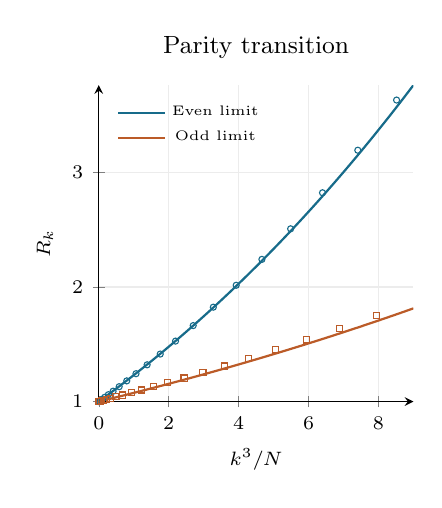
\begin{tikzpicture}
\begin{axis}[width=.46\textwidth,height=5.6cm,xlabel={$k^3/N$},ylabel={$R_k$},title={Parity transition},xmin=0,xmax=9,axis lines=left,grid=major,grid style={gray!15},tick label style={font=\scriptsize},label style={font=\scriptsize},title style={font=\small},legend style={font=\tiny,draw=none,fill=none},legend pos=north west,unbounded coords=jump]
\addplot[draw=proofblue,thick] coordinates {(0,1) (0.0452261306533,1.01006709713) (0.0904522613065,1.02016793118) (0.13567839196,1.03030256997) (0.180904522613,1.04047108142) (0.226130653266,1.05067353354) (0.27135678392,1.06090999446) (0.316582914573,1.07118053238) (0.361809045226,1.08148521562) (0.407035175879,1.09182411258) (0.452261306533,1.10219729177) (0.497487437186,1.1126048218) (0.542713567839,1.12304677136) (0.587939698492,1.13352320927) (0.633165829146,1.14403420442) (0.678391959799,1.1545798258) (0.723618090452,1.16516014252) (0.768844221106,1.17577522377) (0.814070351759,1.18642513885) (0.859296482412,1.19710995715) (0.904522613065,1.20782974816) (0.949748743719,1.21858458148) (0.994974874372,1.22937452679) (1.04020100503,1.2401996539) (1.08542713568,1.25106003268) (1.13065326633,1.26195573313) (1.17587939698,1.27288682534) (1.22110552764,1.28385337949) (1.26633165829,1.29485546589) (1.31155778894,1.30589315492) (1.3567839196,1.31696651707) (1.40201005025,1.32807562293) (1.4472361809,1.33922054319) (1.49246231156,1.35040134865) (1.53768844221,1.36161811019) (1.58291457286,1.37287089881) (1.62814070352,1.38415978561) (1.67336683417,1.39548484178) (1.71859296482,1.40684613861) (1.76381909548,1.41824374751) (1.80904522613,1.42967773997) (1.85427135678,1.44114818759) (1.89949748744,1.45265516208) (1.94472361809,1.46419873524) (1.98994974874,1.47577897898) (2.0351758794,1.48739596529) (2.08040201005,1.4990497663) (2.1256281407,1.51074045421) (2.17085427136,1.52246810135) (2.21608040201,1.53423278011) (2.26130653266,1.54603456303) (2.30653266332,1.55787352272) (2.35175879397,1.56974973191) (2.39698492462,1.58166326343) (2.44221105528,1.59361419021) (2.48743718593,1.60560258527) (2.53266331658,1.61762852176) (2.57788944724,1.62969207291) (2.62311557789,1.64179331207) (2.66834170854,1.65393231268) (2.7135678392,1.6661091483) (2.75879396985,1.67832389258) (2.8040201005,1.69057661927) (2.84924623116,1.70286740224) (2.89447236181,1.71519631545) (2.93969849246,1.72756343297) (2.98492462312,1.73996882898) (3.03015075377,1.75241257776) (3.07537688442,1.76489475369) (3.12060301508,1.77741543125) (3.16582914573,1.78997468504) (3.21105527638,1.80257258976) (3.25628140704,1.8152092202) (3.30150753769,1.82788465129) (3.34673366834,1.84059895802) (3.39195979899,1.85335221553) (3.43718592965,1.86614449902) (3.4824120603,1.87897588384) (3.52763819095,1.89184644541) (3.57286432161,1.90475625928) (3.61809045226,1.91770540109) (3.66331658291,1.9306939466) (3.70854271357,1.94372197167) (3.75376884422,1.95678955226) (3.79899497487,1.96989676444) (3.84422110553,1.98304368439) (3.88944723618,1.9962303884) (3.93467336683,2.00945695285) (3.97989949749,2.02272345426) (4.02512562814,2.03602996921) (4.07035175879,2.04937657443) (4.11557788945,2.06276334673) (4.1608040201,2.07619036304) (4.20603015075,2.0896577004) (4.25125628141,2.10316543595) (4.29648241206,2.11671364694) (4.34170854271,2.13030241072) (4.38693467337,2.14393180476) (4.43216080402,2.15760190664) (4.47738693467,2.17131279404) (4.52261306533,2.18506454474) (4.56783919598,2.19885723665) (4.61306532663,2.21269094777) (4.65829145729,2.22656575622) (4.70351758794,2.24048174023) (4.74874371859,2.25443897812) (4.79396984925,2.26843754834) (4.8391959799,2.28247752944) (4.88442211055,2.29655900008) (4.92964824121,2.31068203903) (4.97487437186,2.32484672518) (5.02010050251,2.3390531375) (5.06532663317,2.35330135511) (5.11055276382,2.3675914572) (5.15577889447,2.3819235231) (5.20100502513,2.39629763223) (5.24623115578,2.41071386414) (5.29145728643,2.42517229847) (5.33668341709,2.43967301499) (5.38190954774,2.45421609356) (5.42713567839,2.46880161417) (5.47236180905,2.4834296569) (5.5175879397,2.49810030196) (5.56281407035,2.51281362966) (5.60804020101,2.52756972044) (5.65326633166,2.54236865482) (5.69849246231,2.55721051345) (5.74371859296,2.57209537709) (5.78894472362,2.58702332661) (5.83417085427,2.601994443) (5.87939698492,2.61700880735) (5.92462311558,2.63206650086) (5.96984924623,2.64716760486) (6.01507537688,2.66231220077) (6.06030150754,2.67750037014) (6.10552763819,2.69273219463) (6.15075376884,2.708007756) (6.1959798995,2.72332713613) (6.24120603015,2.73869041702) (6.2864321608,2.75409768078) (6.33165829146,2.76954900962) (6.37688442211,2.78504448588) (6.42211055276,2.800584192) (6.46733668342,2.81616821055) (6.51256281407,2.83179662421) (6.55778894472,2.84746951574) (6.60301507538,2.86318696807) (6.64824120603,2.8789490642) (6.69346733668,2.89475588727) (6.73869346734,2.91060752051) (6.78391959799,2.92650404729) (6.82914572864,2.94244555107) (6.8743718593,2.95843211546) (6.91959798995,2.97446382413) (6.9648241206,2.99054076093) (7.01005025126,3.00666300977) (7.05527638191,3.0228306547) (7.10050251256,3.03904377989) (7.14572864322,3.05530246961) (7.19095477387,3.07160680825) (7.23618090452,3.08795688033) (7.28140703518,3.10435277047) (7.32663316583,3.1207945634) (7.37185929648,3.13728234399) (7.41708542714,3.15381619721) (7.46231155779,3.17039620814) (7.50753768844,3.18702246199) (7.5527638191,3.20369504408) (7.59798994975,3.22041403986) (7.6432160804,3.23717953486) (7.68844221106,3.25399161477) (7.73366834171,3.27085036537) (7.77889447236,3.28775587257) (7.82412060302,3.30470822239) (7.86934673367,3.32170750098) (7.91457286432,3.33875379458) (7.95979899497,3.35584718958) (8.00502512563,3.37298777246) (8.05025125628,3.39017562985) (8.09547738693,3.40741084846) (8.14070351759,3.42469351514) (8.18592964824,3.44202371686) (8.23115577889,3.45940154071) (8.27638190955,3.47682707388) (8.3216080402,3.4943004037) (8.36683417085,3.5118216176) (8.41206030151,3.52939080315) (8.45728643216,3.54700804802) (8.50251256281,3.56467344) (8.54773869347,3.58238706702) (8.59296482412,3.60014901711) (8.63819095477,3.61795937842) (8.68341708543,3.63581823923) (8.72864321608,3.65372568793) (8.77386934673,3.67168181304) (8.81909547739,3.68968670319) (8.86432160804,3.70774044713) (8.90954773869,3.72584313375) (8.95477386935,3.74399485202) (9,3.76219569108)};
\addlegendentry{Even limit}
\addplot[draw=prooforange,thick] coordinates {(0,1) (0.0452261306533,1.00335345228) (0.0904522613065,1.00671364808) (0.13567839196,1.01008059706) (0.180904522613,1.01345430894) (0.226130653266,1.01683479342) (0.27135678392,1.02022206021) (0.316582914573,1.02361611904) (0.361809045226,1.02701697965) (0.407035175879,1.03042465179) (0.452261306533,1.03383914521) (0.497487437186,1.0372604697) (0.542713567839,1.04068863503) (0.587939698492,1.04412365099) (0.633165829146,1.0475655274) (0.678391959799,1.05101427406) (0.723618090452,1.05446990079) (0.768844221106,1.05793241744) (0.814070351759,1.06140183386) (0.859296482412,1.0648781599) (0.904522613065,1.06836140543) (0.949748743719,1.07185158033) (0.994974874372,1.0753486945) (1.04020100503,1.07885275783) (1.08542713568,1.08236378024) (1.13065326633,1.08588177166) (1.17587939698,1.08940674201) (1.22110552764,1.09293870126) (1.26633165829,1.09647765934) (1.31155778894,1.10002362624) (1.3567839196,1.10357661194) (1.40201005025,1.10713662641) (1.4472361809,1.11070367968) (1.49246231156,1.11427778174) (1.53768844221,1.11785894262) (1.58291457286,1.12144717237) (1.62814070352,1.12504248101) (1.67336683417,1.12864487863) (1.71859296482,1.13225437527) (1.76381909548,1.13587098102) (1.80904522613,1.13949470598) (1.85427135678,1.14312556024) (1.89949748744,1.14676355392) (1.94472361809,1.15040869715) (1.98994974874,1.15406100005) (2.0351758794,1.15772047278) (2.08040201005,1.16138712549) (2.1256281407,1.16506096836) (2.17085427136,1.16874201157) (2.21608040201,1.1724302653) (2.26130653266,1.17612573976) (2.30653266332,1.17982844517) (2.35175879397,1.18353839175) (2.39698492462,1.18725558974) (2.44221105528,1.19098004939) (2.48743718593,1.19471178096) (2.53266331658,1.19845079471) (2.57788944724,1.20219710094) (2.62311557789,1.20595070993) (2.66834170854,1.209711632) (2.7135678392,1.21347987745) (2.75879396985,1.21725545663) (2.8040201005,1.22103837985) (2.84924623116,1.22482865749) (2.89447236181,1.22862629989) (2.93969849246,1.23243131744) (2.98492462312,1.23624372052) (3.03015075377,1.24006351952) (3.07537688442,1.24389072486) (3.12060301508,1.24772534695) (3.16582914573,1.25156739623) (3.21105527638,1.25541688313) (3.25628140704,1.25927381812) (3.30150753769,1.26313821165) (3.34673366834,1.26701007421) (3.39195979899,1.27088941628) (3.43718592965,1.27477624837) (3.4824120603,1.27867058098) (3.52763819095,1.28257242464) (3.57286432161,1.28648178989) (3.61809045226,1.29039868726) (3.66331658291,1.29432312733) (3.70854271357,1.29825512066) (3.75376884422,1.30219467782) (3.79899497487,1.30614180942) (3.84422110553,1.31009652606) (3.88944723618,1.31405883836) (3.93467336683,1.31802875693) (3.97989949749,1.32200629243) (4.02512562814,1.32599145551) (4.07035175879,1.32998425682) (4.11557788945,1.33398470704) (4.1608040201,1.33799281686) (4.20603015075,1.34200859698) (4.25125628141,1.34603205811) (4.29648241206,1.35006321096) (4.34170854271,1.35410206627) (4.38693467337,1.3581486348) (4.43216080402,1.36220292728) (4.47738693467,1.36626495451) (4.52261306533,1.37033472724) (4.56783919598,1.37441225628) (4.61306532663,1.37849755243) (4.65829145729,1.38259062651) (4.70351758794,1.38669148934) (4.74874371859,1.39080015177) (4.79396984925,1.39491662464) (4.8391959799,1.39904091882) (4.88442211055,1.40317304519) (4.92964824121,1.40731301463) (4.97487437186,1.41146083804) (5.02010050251,1.41561652633) (5.06532663317,1.41978009043) (5.11055276382,1.42395154127) (5.15577889447,1.4281308898) (5.20100502513,1.43231814697) (5.24623115578,1.43651332376) (5.29145728643,1.44071643115) (5.33668341709,1.44492748014) (5.38190954774,1.44914648173) (5.42713567839,1.45337344694) (5.47236180905,1.4576083868) (5.5175879397,1.46185131236) (5.56281407035,1.46610223467) (5.60804020101,1.47036116479) (5.65326633166,1.47462811381) (5.69849246231,1.47890309282) (5.74371859296,1.48318611292) (5.78894472362,1.48747718522) (5.83417085427,1.49177632086) (5.87939698492,1.49608353097) (5.92462311558,1.5003988267) (5.96984924623,1.50472221923) (6.01507537688,1.50905371971) (6.06030150754,1.51339333936) (6.10552763819,1.51774108935) (6.15075376884,1.52209698091) (6.1959798995,1.52646102526) (6.24120603015,1.53083323364) (6.2864321608,1.5352136173) (6.33165829146,1.5396021875) (6.37688442211,1.54399895551) (6.42211055276,1.54840393261) (6.46733668342,1.55281713011) (6.51256281407,1.55723855932) (6.55778894472,1.56166823156) (6.60301507538,1.56610615817) (6.64824120603,1.57055235048) (6.69346733668,1.57500681987) (6.73869346734,1.57946957771) (6.78391959799,1.58394063537) (6.82914572864,1.58842000425) (6.8743718593,1.59290769577) (6.91959798995,1.59740372135) (6.9648241206,1.60190809241) (7.01005025126,1.60642082042) (7.05527638191,1.61094191681) (7.10050251256,1.61547139307) (7.14572864322,1.62000926069) (7.19095477387,1.62455553114) (7.23618090452,1.62911021595) (7.28140703518,1.63367332664) (7.32663316583,1.63824487473) (7.37185929648,1.64282487178) (7.41708542714,1.64741332933) (7.46231155779,1.65201025898) (7.50753768844,1.65661567228) (7.5527638191,1.66122958085) (7.59798994975,1.66585199629) (7.6432160804,1.67048293023) (7.68844221106,1.67512239428) (7.73366834171,1.67977040011) (7.77889447236,1.68442695937) (7.82412060302,1.68909208373) (7.86934673367,1.69376578488) (7.91457286432,1.69844807451) (7.95979899497,1.70313896433) (8.00502512563,1.70783846606) (8.05025125628,1.71254659144) (8.09547738693,1.71726335222) (8.14070351759,1.72198876015) (8.18592964824,1.72672282701) (8.23115577889,1.73146556458) (8.27638190955,1.73621698466) (8.3216080402,1.74097709906) (8.36683417085,1.7457459196) (8.41206030151,1.75052345813) (8.45728643216,1.75530972648) (8.50251256281,1.76010473653) (8.54773869347,1.76490850014) (8.59296482412,1.76972102921) (8.63819095477,1.77454233563) (8.68341708543,1.77937243131) (8.72864321608,1.78421132819) (8.77386934673,1.78905903819) (8.81909547739,1.79391557328) (8.86432160804,1.79878094541) (8.90954773869,1.80365516657) (8.95477386935,1.80853824874) (9,1.81343020392)};
\addlegendentry{Odd limit}
\addplot[only marks,mark=o,mark size=1.1pt,draw=proofblue] coordinates {(0.0008,1.00010001) (0.0064,1.00120061024) (0.0216,1.00437277233) (0.0512,1.01069809721) (0.1,1.02127959687) (0.1728,1.03725647552) (0.2744,1.05982311771) (0.4096,1.09025260319) (0.5832,1.12992520916) (0.8,1.18036253312) (1.0648,1.24326808062) (1.3824,1.32057541719) (1.7576,1.41450529323) (2.1952,1.52763352552) (2.7,1.66297187646) (3.2768,1.82406472938) (3.9304,2.0151050435) (4.6656,2.24107391355) (5.4872,2.5079091003) (6.4,2.8227091862) (7.4088,3.19398161243) (8.5184,3.63194484751)};
\addplot[only marks,mark=square,mark size=1.1pt,draw=prooforange] coordinates {(0.0027,1.00030007002) (0.0125,1.00124089051) (0.0343,1.0031850366) (0.0729,1.0064945858) (0.1331,1.01153839995) (0.2197,1.0186957754) (0.3375,1.02836094919) (0.4913,1.04094852341) (0.6859,1.0568998936) (0.9261,1.07669079512) (1.2167,1.1008401154) (1.5625,1.12992016) (1.9683,1.16456860874) (2.4389,1.20550245528) (2.9791,1.25353429247) (3.5937,1.30959138826) (4.2875,1.37473809681) (5.0653,1.45020226958) (5.9319,1.5374064781) (6.8921,1.63800503787) (7.9507,1.75392804084)};
\end{axis}
\end{tikzpicture}\hfill
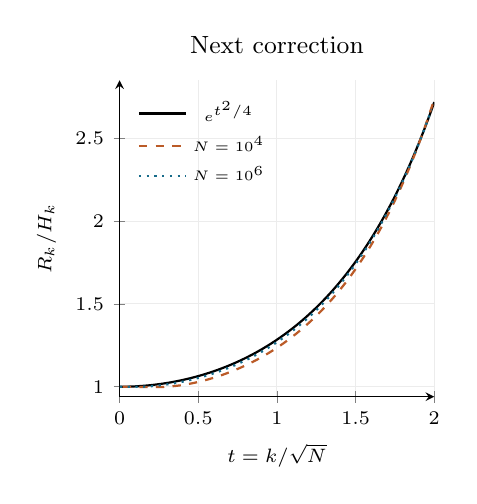
\begin{tikzpicture}
\begin{axis}[width=.46\textwidth,height=5.6cm,xlabel={$t=k/\sqrt N$},ylabel={$R_k/H_k$},title={Next correction},xmin=0,xmax=2,ymin=.94,ymax=2.85,axis lines=left,grid=major,grid style={gray!15},tick label style={font=\scriptsize},label style={font=\scriptsize},title style={font=\small},legend style={font=\tiny,draw=none,fill=none},legend pos=north west,unbounded coords=jump]
\addplot[black,thick] coordinates {(0,1) (0.0100502512563,1.00002525221) (0.0201005025126,1.00010101265) (0.0301507537688,1.00022729282) (0.0402010050251,1.00040411183) (0.0502512562814,1.0006314965) (0.0603015075377,1.00090948128) (0.070351758794,1.00123810832) (0.0804020100503,1.00161742743) (0.0904522613065,1.00204749616) (0.100502512563,1.00252837973) (0.110552763819,1.00306015113) (0.120603015075,1.00364289107) (0.130653266332,1.00427668804) (0.140703517588,1.00496163833) (0.150753768844,1.00569784603) (0.160804020101,1.00648542309) (0.170854271357,1.00732448932) (0.180904522613,1.00821517242) (0.190954773869,1.00915760806) (0.201005025126,1.01015193985) (0.211055276382,1.0111983194) (0.221105527638,1.01229690638) (0.231155778894,1.01344786854) (0.241206030151,1.01465138176) (0.251256281407,1.01590763007) (0.261306532663,1.01721680574) (0.27135678392,1.01857910932) (0.281407035176,1.01999474963) (0.291457286432,1.02146394391) (0.301507537688,1.02298691781) (0.311557788945,1.02456390545) (0.321608040201,1.02619514953) (0.331658291457,1.02788090132) (0.341708542714,1.02962142078) (0.35175879397,1.03141697662) (0.361809045226,1.03326784634) (0.371859296482,1.03517431631) (0.381909547739,1.03713668189) (0.391959798995,1.03915524743) (0.402010050251,1.04123032642) (0.412060301508,1.04336224151) (0.422110552764,1.04555132465) (0.43216080402,1.04779791712) (0.442211055276,1.05010236968) (0.452261306533,1.05246504261) (0.462311557789,1.05488630581) (0.472361809045,1.05736653894) (0.482412060302,1.05990613147) (0.492462311558,1.06250548279) (0.502512562814,1.06516500235) (0.51256281407,1.06788510973) (0.522613065327,1.07066623476) (0.532663316583,1.07350881763) (0.542713567839,1.07641330902) (0.552763819095,1.07938017023) (0.562814070352,1.08240987323) (0.572864321608,1.0855029009) (0.582914572864,1.08865974705) (0.592964824121,1.09188091662) (0.603015075377,1.09516692578) (0.613065326633,1.09851830208) (0.623115577889,1.10193558461) (0.633165829146,1.10541932409) (0.643216080402,1.10897008308) (0.653266331658,1.1125884361) (0.663316582915,1.11627496977) (0.673366834171,1.12003028301) (0.683417085427,1.12385498716) (0.693467336683,1.12774970617) (0.70351758794,1.13171507677) (0.713567839196,1.13575174863) (0.723618090452,1.13986038454) (0.733668341709,1.1440416606) (0.743718592965,1.1482962664) (0.753768844221,1.1526249052) (0.763819095477,1.15702829414) (0.773869346734,1.16150716442) (0.78391959799,1.16606226151) (0.793969849246,1.17069434539) (0.804020100503,1.17540419067) (0.814070351759,1.18019258691) (0.824120603015,1.18506033876) (0.834170854271,1.19000826625) (0.844221105528,1.19503720496) (0.854271356784,1.20014800628) (0.86432160804,1.20534153767) (0.874371859296,1.21061868286) (0.884422110553,1.21598034214) (0.894472361809,1.22142743259) (0.904522613065,1.22696088835) (0.914572864322,1.23258166089) (0.924623115578,1.23829071926) (0.934673366834,1.24408905039) (0.94472361809,1.24997765936) (0.954773869347,1.25595756971) (0.964824120603,1.26202982369) (0.974874371859,1.26819548261) (0.984924623116,1.27445562711) (0.994974874372,1.28081135749) (1.00502512563,1.28726379404) (1.01507537688,1.29381407735) (1.02512562814,1.30046336863) (1.0351758794,1.3072128501) (1.04522613065,1.31406372527) (1.05527638191,1.32101721937) (1.06532663317,1.32807457962) (1.07537688442,1.33523707571) (1.08542713568,1.34250600007) (1.09547738693,1.34988266832) (1.10552763819,1.35736841966) (1.11557788945,1.36496461723) (1.1256281407,1.37267264855) (1.13567839196,1.38049392596) (1.14572864322,1.38842988697) (1.15577889447,1.3964819948) (1.16582914573,1.40465173871) (1.17587939698,1.41294063456) (1.18592964824,1.4213502252) (1.1959798995,1.42988208095) (1.20603015075,1.43853780014) (1.21608040201,1.44731900951) (1.22613065327,1.45622736479) (1.23618090452,1.46526455118) (1.24623115578,1.47443228387) (1.25628140704,1.48373230857) (1.26633165829,1.49316640209) (1.27638190955,1.50273637285) (1.2864321608,1.51244406147) (1.29648241206,1.52229134135) (1.30653266332,1.53228011927) (1.31658291457,1.54241233595) (1.32663316583,1.55268996674) (1.33668341709,1.56311502218) (1.34673366834,1.57368954868) (1.3567839196,1.58441562916) (1.36683417085,1.59529538373) (1.37688442211,1.60633097037) (1.38693467337,1.61752458563) (1.39698492462,1.62887846531) (1.40703517588,1.64039488525) (1.41708542714,1.65207616201) (1.42713567839,1.66392465368) (1.43718592965,1.67594276061) (1.4472361809,1.68813292621) (1.45728643216,1.70049763779) (1.46733668342,1.71303942735) (1.47738693467,1.7257608724) (1.48743718593,1.7386645969) (1.49748743719,1.75175327203) (1.50753768844,1.76502961718) (1.5175879397,1.77849640081) (1.52763819095,1.79215644137) (1.53768844221,1.80601260833) (1.54773869347,1.82006782306) (1.55778894472,1.8343250599) (1.56783919598,1.84878734711) (1.57788944724,1.86345776796) (1.58793969849,1.87833946176) (1.59798994975,1.89343562496) (1.60804020101,1.90874951224) (1.61809045226,1.92428443763) (1.62814070352,1.9400437757) (1.63819095477,1.95603096267) (1.64824120603,1.97224949771) (1.65829145729,1.98870294406) (1.66834170854,2.00539493037) (1.6783919598,2.02232915194) (1.68844221106,2.03950937202) (1.69849246231,2.05693942319) (1.70854271357,2.07462320869) (1.71859296482,2.09256470383) (1.72864321608,2.1107679574) (1.73869346734,2.12923709317) (1.74874371859,2.14797631131) (1.75879396985,2.16698988997) (1.76884422111,2.18628218683) (1.77889447236,2.20585764065) (1.78894472362,2.22572077291) (1.79899497487,2.24587618949) (1.80904522613,2.26632858236) (1.81909547739,2.28708273126) (1.82914572864,2.30814350553) (1.8391959799,2.32951586592) (1.84924623116,2.35120486637) (1.85929648241,2.37321565599) (1.86934673367,2.39555348092) (1.87939698492,2.41822368633) (1.88944723618,2.44123171845) (1.89949748744,2.4645831266) (1.90954773869,2.48828356533) (1.91959798995,2.51233879656) (1.92964824121,2.53675469178) (1.93969849246,2.56153723428) (1.94974874372,2.58669252151) (1.95979899497,2.61222676739) (1.96984924623,2.6381463047) (1.97989949749,2.66445758758) (1.98994974874,2.69116719403) (2,2.71828182846)};
\addlegendentry{$e^{t^2/4}$}
\addplot[draw=prooforange,thick,dashed] coordinates {(0.02,0.99992224078) (0.04,0.999778366154) (0.06,0.999570991992) (0.08,0.999306631385) (0.1,0.998997312678) (0.12,0.998661802035) (0.14,0.998326206019) (0.16,0.998023760864) (0.18,0.997793714777) (0.2,0.997679365193) (0.22,0.997725486183) (0.24,0.997975518618) (0.26,0.998468949102) (0.28,0.999239253437) (0.3,1.00031264413) (0.32,1.0017076862) (0.34,1.00343568495) (0.36,1.00550164253) (0.38,1.00790554023) (0.4,1.01064372083) (0.42,1.01371019771) (0.44,1.01709778191) (0.46,1.02079897694) (0.48,1.02480663604) (0.5,1.02911440495) (0.52,1.03371698706) (0.54,1.03861027208) (0.56,1.04379136667) (0.58,1.04925855951) (0.6,1.0550112468) (0.62,1.06104983728) (0.64,1.06737565051) (0.66,1.07399081704) (0.68,1.08089818629) (0.7,1.08810124473) (0.72,1.09560404583) (0.74,1.10341115163) (0.76,1.11152758532) (0.78,1.11995879381) (0.8,1.12871061908) (0.82,1.13778927701) (0.84,1.14720134271) (0.86,1.15695374098) (0.88,1.16705374133) (0.9,1.17750895655) (0.92,1.18832734423) (0.94,1.19951721073) (0.96,1.21108721724) (0.98,1.22304638735) (1,1.23540411626) (1.02,1.24817018102) (1.04,1.26135475203) (1.06,1.27496840537) (1.08,1.28902213614) (1.1,1.30352737267) (1.12,1.31849599146) (1.14,1.33394033309) (1.16,1.34987321882) (1.18,1.36630796815) (1.2,1.38325841715) (1.22,1.40073893769) (1.24,1.41876445758) (1.26,1.43735048168) (1.28,1.45651311396) (1.3,1.47626908055) (1.32,1.49663575392) (1.34,1.51763117813) (1.36,1.53927409525) (1.38,1.56158397296) (1.4,1.58458103349) (1.42,1.60828628382) (1.44,1.6327215473) (1.46,1.65790949671) (1.48,1.68387368889) (1.5,1.71063860091) (1.52,1.73822966792) (1.54,1.76667332283) (1.56,1.7959970377) (1.58,1.82622936721) (1.6,1.85739999404) (1.62,1.88953977642) (1.64,1.92268079793) (1.66,1.95685641957) (1.68,1.99210133437) (1.7,2.02845162455) (1.72,2.06594482132) (1.74,2.10461996768) (1.76,2.14451768402) (1.78,2.18568023701) (1.8,2.2281516117) (1.82,2.27197758716) (1.84,2.31720581569) (1.86,2.36388590589) (1.88,2.41206950981) (1.9,2.46181041425) (1.92,2.51316463658) (1.94,2.56619052522) (1.96,2.62094886508) (1.98,2.67750298817) (2,2.73591888967)};
\addlegendentry{$N=10^4$}
\addplot[draw=proofblue,thick,dotted] coordinates {(0.002,0.999999222224) (0.022,0.999955042977) (0.042,0.999850189734) (0.062,0.999710020383) (0.082,0.999590402406) (0.102,0.999574341399) (0.122,0.99975267191) (0.142,1.0001992924) (0.162,1.00095596584) (0.182,1.00203281715) (0.202,1.00341905545) (0.222,1.00509510259) (0.242,1.00704102512) (0.262,1.00924057219) (0.282,1.01168218194) (0.302,1.01435848925) (0.322,1.01726535266) (0.342,1.02040090537) (0.362,1.02376481003) (0.382,1.02735773723) (0.402,1.03118102695) (0.422,1.03523648067) (0.442,1.03952623906) (0.462,1.04405271262) (0.482,1.04881854351) (0.502,1.0538265853) (0.522,1.05907989264) (0.542,1.06458171655) (0.562,1.07033550281) (0.582,1.07634489213) (0.602,1.0826137216) (0.622,1.08914602686) (0.642,1.09594604492) (0.662,1.10301821751) (0.682,1.11036719484) (0.702,1.11799783981) (0.722,1.12591523264) (0.742,1.13412467581) (0.762,1.14263169945) (0.782,1.15144206703) (0.802,1.16056178142) (0.822,1.16999709138) (0.842,1.17975449833) (0.862,1.18984076352) (0.882,1.20026291557) (0.902,1.21102825843) (0.922,1.22214437968) (0.942,1.23361915923) (0.962,1.24546077848) (0.982,1.25767772985) (1.002,1.27027882682) (1.022,1.28327321431) (1.042,1.29667037966) (1.062,1.31048016397) (1.082,1.32471277406) (1.102,1.33937879487) (1.122,1.35448920243) (1.142,1.37005537741) (1.162,1.38608911922) (1.182,1.40260266077) (1.202,1.41960868382) (1.222,1.43712033503) (1.242,1.45515124265) (1.262,1.473715534) (1.282,1.49282785365) (1.302,1.51250338237) (1.322,1.53275785697) (1.342,1.55360759088) (1.362,1.57506949574) (1.382,1.59716110384) (1.402,1.61990059151) (1.422,1.64330680363) (1.442,1.66739927909) (1.462,1.69219827737) (1.482,1.71772480636) (1.502,1.74400065127) (1.522,1.77104840488) (1.542,1.7988914991) (1.562,1.82755423788) (1.582,1.85706183158) (1.602,1.88744043284) (1.622,1.91871717409) (1.642,1.95092020659) (1.662,1.98407874133) (1.682,2.01822309167) (1.702,2.05338471787) (1.722,2.08959627365) (1.742,2.12689165481) (1.762,2.16530604999) (1.782,2.2048759938) (1.802,2.2456394222) (1.822,2.28763573057) (1.842,2.33090583423) (1.862,2.37549223179) (1.882,2.42143907143) (1.902,2.46879222008) (1.922,2.51759933589) (1.942,2.56790994395) (1.962,2.61977551552) (1.982,2.67324955095)};
\addlegendentry{$N=10^6$}
\end{axis}
\end{tikzpicture}
\caption{The two transitions. Left: the parity-dependent critical limits and recurrence evaluations at $N=10^4$. Right: the ratio to the hyperbolic approximation at even orders, compared with its square-root correction. Curves illustrate the proved statements and are not premises of the proofs.}
\label{fig:regimes}
\end{figure}


\clearpage
\section{The sublinear range and a formula at every order}\label{sec:asymptotics}

The square-root correction is the first term of a convergent exponent. Retaining that exponent describes every sublinear order. Keeping the permutation denominator exact then gives one formula throughout the full range $2\le k\le N$.

Define, for $0\le t<1$,
\begin{equation}\label{eq:actionG}
G(t)=t+\frac{t^2}{2}+(1-t^2)\log(1-t)-\frac23t^3
=\sum_{j\ge4}\frac{2t^j}{j(j-2)}.
\end{equation}
All coefficients in the last series are positive.

\begin{theorem}[Uniform sublinear approximation]\label{thm:sublinear}
For every sequence $b_N=o(N)$ with $b_N\ge2$,
\begin{equation}\label{eq:sublinear}
\sup_{2\le k\le b_N}
\left|\frac{R_k}{H_k\exp\{NG(\sqrt{k/N})\}}-1\right|
\longrightarrow0.
\end{equation}
The supremum is over integers. The definition of $H_k$ remains \eqref{eq:hyperdef}, including $K=k-1$ at odd orders.
\end{theorem}

\begin{corollary}[Sharp thresholds for successive corrections]\label{cor:hierarchy}
For a fixed integer $p\ge4$, put
\[
G_p(t)=\sum_{j=4}^{p}\frac{2t^j}{j(j-2)}.
\]
Along any sequence $2\le k=o(N)$,
\begin{equation}\label{eq:hierarchy}
\frac{R_k}{H_ke^{NG_p(\sqrt{k/N})}}\longrightarrow1
\quad\Longleftrightarrow\quad
k=o\left(N^{(p-1)/(p+1)}\right).
\end{equation}
The ratio stays bounded exactly when $k^{p+1}/N^{p-1}$ stays bounded. At $k/N^{(p-1)/(p+1)}\to c\in(0,\infty)$ its limit is
\begin{equation}\label{eq:hierarchyboundary}
\exp\left(\frac{2c^{(p+1)/2}}{(p+1)(p-1)}\right).
\end{equation}
In particular, the correction $e^{k^2/(4N)}$ is relatively accurate up to $k=o(N^{3/5})$. Adding $2k^{5/2}/(15N^{3/2})$ to its exponent extends that range to $k=o(N^{2/3})$.
\end{corollary}

The thresholds in \eqref{eq:hierarchy} are uniform upper-range statements as well: the relative error tends uniformly to zero on $2\le k\le b_N$ whenever $b_N=o(N^{(p-1)/(p+1)})$. The conclusion concerns each fixed truncation degree $p$.

\subsection{A coefficient estimate with both angular peaks controlled}

Write
\[
f(z)=\frac{z}{1-z}+\log(1-z),\qquad
x=\sqrt{K/N},\qquad r=\frac{x}{1+x}.
\]
The positive saddle and its variance parameter are explicit:
\begin{equation}\label{eq:saddleequation}
Nrf'(r)=\frac{Nr^2}{(1-r)^2}=K,\qquad
b=N(r\partial_r)^2f(r)=2K(1+x).
\end{equation}

\begin{lemma}[Uniform positive-saddle estimate]\label{lem:saddle}
Let $2\le K\le N$ be integers, $\epsilon\in\{0,1\}$ and $K+\epsilon\le N$. Put $\lambda=(2/3)Nx^3$. There is an absolute constant $C$ such that
\begin{equation}\label{eq:saddlecoefficient}
[z^{K+\epsilon}]e^{Nf(z)}
=\frac{e^{Nf(r)}r^{-K-\epsilon}}{\sqrt{2\pi b}}(1+E),
\qquad |E|\le C\left(K^{-1}+e^{-\lambda/8}\right).
\end{equation}
The right side is a relative approximation when $K$ and $\lambda$ diverge. The bound remains valid without that divergence.
\end{lemma}
\begin{proof}
Cauchy's formula reduces the normalized coefficient to
\[
\frac1{2\pi}\int_{-\pi}^{\pi}
e^{\Phi(\theta)-i\epsilon\theta}\,d\theta,
\qquad
\Phi(\theta)=N(f(re^{i\theta})-f(r))-iK\theta.
\]
The positive coefficients of $f$ give
\begin{equation}\label{eq:angulardamping}
-\Re\Phi(\theta)
\ge Nr^2\sin^2\theta+\frac23Nr^3(1-\cos3\theta).
\end{equation}
Here $r\le1/2$ and $Nr^2=K/(1+x)^2\ge K/4$. On $|\theta|\le\pi/6$,
\[
\Re\Phi(\theta)\le-\frac9{4\pi^2}K\theta^2.
\]
For each fixed $q\ge2$, the derivative sum
\[
N\sum_{j\ge2}\frac{j-1}{j}j^qr^j
\le K\sum_{j\ge2}\frac{j-1}{j}j^q2^{2-j}
\]
is bounded by an absolute constant depending only on $q$, times $K$. Taylor's inequalities and \eqref{eq:saddleequation} therefore give
\[
\Re\Phi=-b\theta^2/2+O(K\theta^4),\qquad
|\Im\Phi|\le CK|\theta|^3.
\]
Pair conjugate angles. The central integrand becomes
$e^{\Re\Phi}\cos(\Im\Phi-\epsilon\theta)$. Using
$|\cos u-1|\le u^2/2$ and the real exponential mean-value bound, its difference from $e^{-b\theta^2/2}$ is at most
\[
C(K\theta^4+K^2\theta^6+\theta^2)e^{-cK\theta^2}.
\]
Its integral is $O(K^{-3/2})$, whereas the Gaussian integral is of order $K^{-1/2}$. The Gaussian tails outside the central interval are exponentially small.

The pair term alone does not suppress the other peak. Write $\theta=\pi+u$ modulo $2\pi$, with $|u|\le\pi/6$. Then
\[
1-\cos3\theta=1+\cos3u\ge1,\qquad
\frac23Nr^3=\frac\lambda{(1+x)^3}\ge\frac\lambda8.
\]
The pair term in \eqref{eq:angulardamping} supplies Gaussian decay in $u$. The second-peak integral is therefore at most $CK^{-1/2}e^{-\lambda/8}$. At the remaining angles, $|\sin\theta|\ge1/2$ and the integral is at most $Ce^{-K/16}$. Dividing by the central Gaussian integral proves \eqref{eq:saddlecoefficient}. The circle $r\le1/2$ stays away from the singularity at one, including at $K=N$.
\end{proof}

\subsection{Restoring parity and the permutation denominator}

For the moment normalization take $K=2\lfloor k/2\rfloor=2m$ and $\epsilon=k-K$. Set
\begin{equation}\label{eq:actionq}
h(x)=x+(x^2-1)\log(1+x)-\frac{x^2}{2},\qquad
q(x)=h(x)-\frac23x^3.
\end{equation}
The action identity is exact:
\[
Nf(r)-K\log r+K\log x-K/2=Nh(x).
\]
Stirling's formula applied to $m!$ in $\mathcal L_k$, followed by Lemma~\ref{lem:saddle}, gives
\begin{equation}\label{eq:normalizedsaddle}
\frac{Q_k}{\mathcal L_k}
=\frac{e^{Nh(x)}(1+x)^{\epsilon-1/2}}{2\lambda^\epsilon}
\left[1+O\left(K^{-1}+e^{-\lambda/8}\right)\right].
\end{equation}
Indeed, the even factorial cancellation leaves $2^mm!N^{-m}$ times the coefficient. At odd orders the additional factor is exactly
\[
\frac3{2Kr}=\frac{1+x}{\lambda}.
\]
Thus no odd-order shift is lost. The exact hyperbolic term is
$H_k=(e^\lambda+(-1)^\epsilon e^{-\lambda})/(2\lambda^\epsilon)$.
When $K$ and $\lambda$ exceed sufficiently large fixed constants, taking logarithms in \eqref{eq:normalizedsaddle} yields
\begin{equation}\label{eq:logsaddle}
\log\frac{R_k}{H_k}
=\log D_k+Nq(x)+(\epsilon-1/2)\log(1+x)
+O\left(K^{-1}+e^{-\lambda/8}\right).
\end{equation}

For the sublinear formula, put $t=\sqrt{k/N}$ and
$I(u)=u+(1-u)\log(1-u)$. Monotonicity of $-\log(1-v)$ bounds its left Riemann sum by
\begin{equation}\label{eq:denominatorintegral}
0\le NI(k/N)-\log D_k\le-\log(1-k/N).
\end{equation}
The derivative identities
$h'(x)=2x\log(1+x)$ and $q'(x)=2x(\log(1+x)-x)$ give $|q'(x)|\le x^3$. Since $t^2-x^2=\epsilon/N$,
$N|q(t)-q(x)|\le k/N$. Finally, $I(t^2)+q(t)=G(t)$ exactly. Hence, uniformly for $k/N\le1/16$ under the same large-$K$, large-$\lambda$ conditions,
\begin{equation}\label{eq:logsublinear}
\log\frac{R_k}{H_k}
=NG(\sqrt{k/N})+(\epsilon-1/2)\log(1+\sqrt{K/N})
+O\left(k/N+K^{-1}+e^{-\lambda/8}\right).
\end{equation}
The parity term has order $\sqrt{k/N}$ and must be retained for finer error estimates.

\begin{proof}[Proof of Theorem~\ref{thm:sublinear}]
On $\sqrt N<k\le b_N=o(N)$, the minimum $K$ is of order $\sqrt N$ and the minimum $\lambda$ is of order $N^{1/4}$. Every error in \eqref{eq:logsublinear}, and its explicit parity term, tends uniformly to zero. On $2\le k\le\sqrt N$, Theorem~\ref{thm:sqrt} applies, while the positive series \eqref{eq:actionG} gives
\[
0\le NG(\sqrt{k/N})-\frac{k^2}{4N}
\le C\frac{k^{5/2}}{N^{3/2}}\le CN^{-1/4}.
\]
This patches the two ranges and includes fixed orders. It does not assume a single-saddle relative approximation when $\lambda$ is small.
\end{proof}

\begin{proof}[Proof of Corollary~\ref{cor:hierarchy}]
For fixed $p$, positivity and decreasing coefficients give
\[
G(t)-G_p(t)=\frac{2t^{p+1}}{(p+1)(p-1)}(1+O_p(t))
\quad(t\to0).
\]
The first term bounds the tail from below, and the same term divided by $1-t$ bounds it from above. Theorem~\ref{thm:sublinear} therefore gives
\[
\log\frac{R_k}{H_ke^{NG_p(\sqrt{k/N})}}
=\frac{2k^{(p+1)/2}}{(p+1)(p-1)N^{(p-1)/2}}
\bigl(1+O_p(\sqrt{k/N})\bigr)+o(1).
\]
This proves relative accuracy, its necessity, boundedness and the boundary limit. The same positive-tail bound proves uniformity over the stated upper ranges. In particular,
\[
NG(\sqrt{k/N})
=\frac{k^2}{4N}+\frac{2k^{5/2}}{15N^{3/2}}
+\frac{k^3}{12N^2}+\frac{2k^{7/2}}{35N^{5/2}}+\cdots.
\]
The coefficient $2/15$ combines block weights, pair depletion and the permutation denominator. It is not the raw weight of a single five-element block.
\end{proof}

\subsection{Keeping the denominator exact}

For $2\le k\le N$, define
\begin{equation}\label{eq:globalformula}
\mathcal A_{N,k}
=D_kH_k e^{Nq(\sqrt{K/N})}
(1+\sqrt{K/N})^{\epsilon-1/2}.
\end{equation}
Every factor is positive and finite, including at $k=N$. Write
\[
\mathcal E_{N,k}=\frac{R_k}{\mathcal A_{N,k}}-1.
\]
The full exponent and the parity amplitude in \eqref{eq:globalformula} give a sharper global rate than the quartically corrected approximation considered in the next section. Its largest error occurs at cubic orders.

For $c>0$, put
\begin{equation}\label{eq:globalprofiledef}
\begin{gathered}
\ell(c)=\frac23c^{3/2},\qquad
p_0(t)=t\tanh t,\qquad p_1(t)=t\coth t-1,\\
\Phi_\epsilon(c)=\frac{3(2\epsilon-1)}{4c}
\bigl(p_\epsilon(\ell(c))-\ell(c)\bigr).
\end{gathered}
\end{equation}
Both profiles extend continuously to zero with value zero.

\begin{theorem}[Sharp uniform approximation at every order]\label{thm:global}
As $N\to\infty$,
\begin{equation}\label{eq:globalerror}
\sup_{2\le k\le N}|\mathcal E_{N,k}|
=C_*N^{-1/3}+o(N^{-1/3}),
\end{equation}
where the positive absolute constant is
\begin{equation}\label{eq:globalsharpconstant}
C_*=\max_{c>0}\frac3{4c}
\left(1-\frac{2\ell(c)}{e^{2\ell(c)}-1}\right).
\end{equation}
More precisely, the full-range parity profile satisfies
\begin{equation}\label{eq:globalprofile}
\sup_{2\le k\le N}
\left|N^{1/3}\mathcal E_{N,k}
-\Phi_{k\bmod2}(k/N^{1/3})\right|\longrightarrow0.
\end{equation}
Uniformly for $\sqrt N\le k\le N$, the error is
$O(K^{-1}+e^{-\lambda/8})$, and hence $O(N^{-1/2})$.

The maximum in \eqref{eq:globalsharpconstant} is attained at a unique $c_*>0$. If $z_*$ is the unique positive root of
\begin{equation}\label{eq:globalmaxequation}
2e^{2z}-(3z^2-z+4)e^z-z+2=0,
\end{equation}
then $c_*=(3z_*/4)^{2/3}$. Numerically,
\[
c_*\approx1.16540187318,\qquad C_*\approx0.395496270091.
\]
Odd orders nearest $c_*N^{1/3}$ attain the limiting supremum, with negative signed error. In particular, the exponent $1/3$ in \eqref{eq:globalerror} is optimal for \eqref{eq:globalformula}.
\end{theorem}
\begin{proof}
Appendix~\ref{sec:globalsharpproof} proves the compact critical expansion \eqref{eq:globalcompact}, retains both real saddle contributions, and controls both tails of $k/N^{1/3}$. These estimates give \eqref{eq:globalprofile}. The odd absolute profile strictly exceeds the even profile, and the appendix proves uniqueness of its maximizer, yielding \eqref{eq:globalerror} and \eqref{eq:globalsharpconstant}.

For the upper-range bound, divide \eqref{eq:normalizedsaddle} by the exact $H_k$. The residual factor is $(1+(-1)^\epsilon e^{-2\lambda})^{-1}$, which differs from one exponentially little for $k\ge\sqrt N$. The factor $D_k$ cancels exactly. This also explains why no approximation to $(N)_k$ is needed at $k=N$.
\end{proof}

At cubic orders, the four-block term and the common quadratic availability loss cancel between the moment and \eqref{eq:globalformula}. The remaining error records the difference between the mean shifted triple count $J-\epsilon$ and the Poisson parameter $\lambda$. The shift removes the compulsory triple at odd orders. Its contribution is divided by $K$, and its signs are opposite in the two parities. The uniform $N^{-1/4}$ rate in the next section concerns the different approximation $e^{k^2/(4N)}H_k$.

At the top order, Lemma~\ref{lem:saddle} can be used with degree $K=N$ and offset zero, without a parity restriction on that lemma. Here $r=1/2$ and $b=4N$, giving
\[
[z^N]e^{Nf(z)}=\frac{e^N}{\sqrt{8\pi N}}(1+O(N^{-1})),\qquad
a_N(N)=\frac{1+O(N^{-1})}{2N!}.
\]
This endpoint also follows from the classical truncated-exponential identity for $L_N^{(-N-1)}$. It is a consistency check on the full-range formula, rather than a separate priority claim.

\begin{figure}[htbp]
\centering
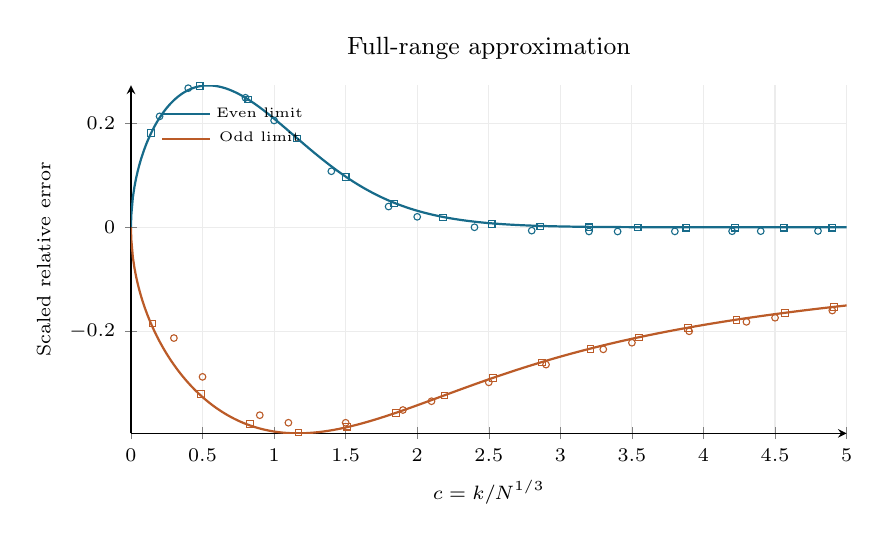
\begin{tikzpicture}
\begin{axis}[width=.88\textwidth,height=6cm,xlabel={$c=k/N^{1/3}$},ylabel={Scaled relative error},title={Full-range approximation},xmin=0,xmax=5,axis lines=left,grid=major,grid style={gray!15},tick label style={font=\scriptsize},label style={font=\scriptsize},title style={font=\small},legend style={font=\tiny,draw=none,fill=none},legend pos=north west,unbounded coords=jump]
\addplot[draw=proofblue,thick] coordinates {(0,0) (0.002,0.0223593464417) (0.013131403118,0.0572386893356) (0.0242628062361,0.0776863864645) (0.0353942093541,0.0936491634537) (0.0465256124722,0.107127449485) (0.0576570155902,0.118951297532) (0.0687884187082,0.129560525578) (0.0799198218263,0.139221571995) (0.0910512249443,0.148110344713) (0.102182628062,0.156350208148) (0.11331403118,0.164031646809) (0.124445434298,0.171223373591) (0.135576837416,0.177979035256) (0.146708240535,0.184341477052) (0.157839643653,0.190345571965) (0.168971046771,0.19602016444) (0.180102449889,0.201389445536) (0.191233853007,0.206473950581) (0.202365256125,0.211291298807) (0.213496659243,0.21585675219) (0.224628062361,0.220183644801) (0.235759465479,0.2242837176) (0.246890868597,0.228167382989) (0.258022271715,0.231843936371) (0.269153674833,0.235321727175) (0.280285077951,0.238608298477) (0.291416481069,0.241710502019) (0.302547884187,0.244634593736) (0.313679287305,0.247386313707) (0.324810690423,0.249970953542) (0.335942093541,0.252393413533) (0.347073496659,0.254658251432) (0.358204899777,0.256769724309) (0.369336302895,0.258731824651) (0.380467706013,0.260548311652) (0.391599109131,0.262222738451) (0.402730512249,0.263758475938) (0.413861915367,0.265158733642) (0.424993318486,0.266426578124) (0.436124721604,0.267564949218) (0.447256124722,0.268576674416) (0.45838752784,0.269464481642) (0.469518930958,0.270231010622) (0.480650334076,0.270878823022) (0.491781737194,0.271410411502) (0.502913140312,0.271828207813) (0.51404454343,0.272134590046) (0.525175946548,0.272331889128) (0.536307349666,0.272422394636) (0.547438752784,0.272408360011) (0.558570155902,0.272292007222) (0.56970155902,0.272075530937) (0.580832962138,0.271761102248) (0.591964365256,0.271350871988) (0.603095768374,0.270846973676) (0.614227171492,0.270251526121) (0.62535857461,0.269566635714) (0.636489977728,0.268794398433) (0.647621380846,0.267936901584) (0.658752783964,0.266996225291) (0.669884187082,0.265974443767) (0.6810155902,0.264873626368) (0.692146993318,0.263695838455) (0.703278396437,0.262443142067) (0.714409799555,0.261117596437) (0.725541202673,0.259721258334) (0.736672605791,0.258256182276) (0.747804008909,0.256724420587) (0.758935412027,0.255128023341) (0.770066815145,0.253469038183) (0.781198218263,0.251749510037) (0.792329621381,0.249971480716) (0.803461024499,0.248136988434) (0.814592427617,0.246248067237) (0.825723830735,0.24430674635) (0.836855233853,0.24231504945) (0.847986636971,0.240274993874) (0.859118040089,0.238188589774) (0.870249443207,0.236057839203) (0.881380846325,0.233884735173) (0.892512249443,0.231671260651) (0.903643652561,0.229419387538) (0.914775055679,0.227131075602) (0.925906458797,0.224808271397) (0.937037861915,0.222452907154) (0.948169265033,0.220066899665) (0.959300668151,0.21765214915) (0.970432071269,0.215210538123) (0.981563474388,0.212743930256) (0.992694877506,0.210254169249) (1.00382628062,0.207743077704) (1.01495768374,0.205212456017) (1.02608908686,0.20266408128) (1.03722048998,0.200099706207) (1.0483518931,0.197521058085) (1.05948329621,0.194929837743) (1.07061469933,0.192327718564) (1.08174610245,0.189716345516) (1.09287750557,0.187097334233) (1.10400890869,0.184472270119) (1.1151403118,0.181842707505) (1.12627171492,0.179210168844) (1.13740311804,0.176576143948) (1.14853452116,0.173942089274) (1.15966592428,0.171309427258) (1.17079732739,0.168679545698) (1.18192873051,0.166053797189) (1.19306013363,0.163433498602) (1.20419153675,0.160819930622) (1.21532293987,0.158214337338) (1.22645434298,0.155617925884) (1.2375857461,0.15303186613) (1.24871714922,0.150457290429) (1.25984855234,0.147895293421) (1.27097995546,0.145346931878) (1.28211135857,0.142813224613) (1.29324276169,0.140295152431) (1.30437416481,0.137793658136) (1.31550556793,0.135309646583) (1.32663697105,0.132843984783) (1.33776837416,0.130397502051) (1.34889977728,0.127970990201) (1.3600311804,0.12556520379) (1.37116258352,0.123180860395) (1.38229398664,0.120818640941) (1.39342538976,0.118479190065) (1.40455679287,0.116163116519) (1.41568819599,0.113870993605) (1.42681959911,0.111603359652) (1.43795100223,0.109360718521) (1.44908240535,0.107143540143) (1.46021380846,0.104952261081) (1.47134521158,0.102787285127) (1.4824766147,0.10064898392) (1.49360801782,0.0985376975839) (1.50473942094,0.0964537353959) (1.51587082405,0.0943973764643) (1.52700222717,0.0923688704311) (1.53813363029,0.090368438187) (1.54926503341,0.0883962726019) (1.56039643653,0.0864525392666) (1.57152783964,0.0845373772457) (1.58265924276,0.0826508998389) (1.59379064588,0.0807931953497) (1.604922049,0.0789643278588) (1.61605345212,0.0771643380029) (1.62718485523,0.0753932437543) (1.63831625835,0.0736510412029) (1.64944766147,0.071937705337) (1.66057906459,0.0702531908222) (1.67171046771,0.0685974327785) (1.68284187082,0.0669703475516) (1.69397327394,0.0653718334801) (1.70510467706,0.0638017716558) (1.71623608018,0.0622600266763) (1.7273674833,0.0607464473901) (1.73849888641,0.0592608676312) (1.74963028953,0.0578031069443) (1.76076169265,0.0563729712993) (1.77189309577,0.0549702537937) (1.78302449889,0.0535947353428) (1.794155902,0.052246185357) (1.80528730512,0.0509243624063) (1.81641870824,0.04962901487) (1.82755011136,0.0483598815729) (1.83868151448,0.0471166924059) (1.84981291759,0.0458991689325) (1.86094432071,0.0447070249793) (1.87207572383,0.0435399672114) (1.88320712695,0.0423976956914) (1.89433853007,0.0412799044235) (1.90546993318,0.0401862818801) (1.9166013363,0.0391165115141) (1.92773273942,0.0380702722535) (1.93886414254,0.0370472389806) (1.94999554566,0.0360470829948) (1.96112694878,0.0350694724599) (1.97225835189,0.0341140728347) (1.98338975501,0.0331805472877) (1.99452115813,0.032268557097) (2.00565256125,0.0313777620337) (2.01678396437,0.0305078207302) (2.02791536748,0.0296583910334) (2.0390467706,0.0288291303428) (2.05017817372,0.0280196959343) (2.06130957684,0.0272297452684) (2.07244097996,0.0264589362856) (2.08357238307,0.0257069276869) (2.09470378619,0.0249733792011) (2.10583518931,0.024257951838) (2.11696659243,0.0235603081299) (2.12809799555,0.0228801123588) (2.13922939866,0.0222170307724) (2.15036080178,0.0215707317871) (2.1614922049,0.0209408861801) (2.17262360802,0.0203271672687) (2.18375501114,0.0197292510801) (2.19488641425,0.0191468165092) (2.20601781737,0.0185795454662) (2.21714922049,0.0180271230145) (2.22828062361,0.017489237498) (2.23941202673,0.0169655806598) (2.25054342984,0.016455847751) (2.26167483296,0.015959737631) (2.27280623608,0.0154769528593) (2.2839376392,0.0150071997787) (2.29506904232,0.0145501885916) (2.30620044543,0.0141056334272) (2.31733184855,0.0136732524028) (2.32846325167,0.0132527676773) (2.33959465479,0.0128439054983) (2.35072605791,0.0124463962426) (2.36185746102,0.0120599744508) (2.37298886414,0.0116843788559) (2.38412026726,0.0113193524064) (2.39525167038,0.0109646422835) (2.4063830735,0.0106199999144) (2.41751447661,0.0102851809793) (2.42864587973,0.00995994541509) (2.43977728285,0.0096440574139) (2.45090868597,0.00933728541774) (2.46204008909,0.00903940210925) (2.4731714922,0.00875018439874) (2.48430289532,0.00846941340768) (2.49543429844,0.00819687444898) (2.50656570156,0.00793235700408) (2.51769710468,0.00767565469723) (2.5288285078,0.00742656526693) (2.53995991091,0.00718489053491) (2.55109131403,0.00695043637267) (2.56222271715,0.00672301266584) (2.57335412027,0.00650243327642) (2.58448552339,0.00628851600315) (2.5956169265,0.00608108254011) (2.60674832962,0.00587995843366) (2.61787973274,0.00568497303787) (2.62901113586,0.00549595946868) (2.64014253898,0.00531275455669) (2.65127394209,0.00513519879888) (2.66240534521,0.00496313630934) (2.67353674833,0.00479641476903) (2.68466815145,0.00463488537481) (2.69579955457,0.00447840278765) (2.70693095768,0.00432682508037) (2.7180623608,0.00418001368475) (2.72919376392,0.0040378333382) (2.74032516704,0.00390015203017) (2.75145657016,0.00376684094814) (2.76258797327,0.00363777442351) (2.77371937639,0.00351282987729) (2.78485077951,0.00339188776573) (2.79598218263,0.00327483152594) (2.80711358575,0.00316154752152) (2.81824498886,0.00305192498837) (2.82937639198,0.00294585598053) (2.8405077951,0.00284323531633) (2.85163919822,0.0027439605247) (2.86277060134,0.00264793179184) (2.87390200445,0.00255505190814) (2.88503340757,0.00246522621553) (2.89616481069,0.0023783625552) (2.90729621381,0.00229437121575) (2.91842761693,0.00221316488179) (2.92955902004,0.00213465858307) (2.94069042316,0.00205876964409) (2.95182182628,0.00198541763426) (2.9629532294,0.00191452431863) (2.97408463252,0.00184601360919) (2.98521603563,0.00177981151675) (2.99634743875,0.0017158461035) (3.00747884187,0.00165404743612) (3.01861024499,0.00159434753961) (3.02974164811,0.00153668035172) (3.04087305122,0.00148098167804) (3.05200445434,0.00142718914786) (3.06313585746,0.00137524217057) (3.07426726058,0.00132508189289) (3.0853986637,0.00127665115666) (3.09653006682,0.00122989445749) (3.10766146993,0.00118475790395) (3.11879287305,0.00114118917755) (3.12992427617,0.00109913749347) (3.14105567929,0.00105855356188) (3.15218708241,0.00101938955009) (3.16331848552,0.000981599045282) (3.17444988864,0.000945137018098) (3.18558129176,0.000909959786783) (3.19671269488,0.000876024982123) (3.207844098,0.000843291513043) (3.21897550111,0.000811719532907) (3.23010690423,0.000781270406497) (3.24123830735,0.000751906677685) (3.25236971047,0.000723592037778) (3.26350111359,0.000696291294528) (3.2746325167,0.000669970341817) (3.28576391982,0.000644596129992) (3.29689532294,0.000620136636855) (3.30802672606,0.000596560839292) (3.31915812918,0.000573838685547) (3.33028953229,0.00055194106811) (3.34142093541,0.000530839797241) (3.35255233853,0.000510507575092) (3.36368374165,0.000490917970437) (3.37481514477,0.000472045394004) (3.38594654788,0.000453865074377) (3.397077951,0.000436353034489) (3.40820935412,0.000419486068678) (3.41934075724,0.000403241720296) (3.43047216036,0.000387598259879) (3.44160356347,0.000372534663846) (3.45273496659,0.000358030593735) (3.46386636971,0.000344066375964) (3.47499777283,0.00033062298209) (3.48612917595,0.000317682009593) (3.49726057906,0.000305225663131) (3.50839198218,0.000293236736296) (3.5195233853,0.000281698593837) (3.53065478842,0.000270595154352) (3.54178619154,0.000259910873432) (3.55291759465,0.000249630727258) (3.56404899777,0.000239740196634) (3.57518040089,0.000230225251445) (3.58631180401,0.000221072335545) (3.59744320713,0.000212268352046) (3.60857461024,0.000203800649013) (3.61970601336,0.000195657005557) (3.63083741648,0.000187825618304) (3.6419688196,0.00018029508825) (3.65310022272,0.000173054407978) (3.66423162584,0.000166092949235) (3.67536302895,0.000159400450863) (3.68649443207,0.000152967007069) (3.69762583519,0.000146783056034) (3.70875723831,0.000140839368851) (3.71988864143,0.000135127038771) (3.73102004454,0.000129637470779) (3.74215144766,0.000124362371454) (3.75328285078,0.000119293739144) (3.7644142539,0.000114423854415) (3.77554565702,0.000109745270794) (3.78667706013,0.000105250805779) (3.79780846325,0.000100933532122) (3.80893986637,9.67867693696e-05) (3.82007126949,9.28040756616e-05) (3.83120267261,8.89792397743e-05) (3.84233407572,8.53062734075e-05) (3.85346547884,8.17794037055e-05) (3.86459688196,7.8393066008e-05) (3.87572828508,7.51418968226e-05) (3.8868596882,7.20207270153e-05) (3.89799109131,6.90245752112e-05) (3.90912249443,6.61486414011e-05) (3.92025389755,6.33883007474e-05) (3.93138530067,6.07390975845e-05) (3.94251670379,5.81967396076e-05) (3.9536481069,5.57570922461e-05) (3.96477951002,5.34161732138e-05) (3.97591091314,5.11701472345e-05) (3.98704231626,4.90153209349e-05) (3.99817371938,4.69481379011e-05) (4.00930512249,4.49651738957e-05) (4.02043652561,4.30631322274e-05) (4.03156792873,4.12388392722e-05) (4.04269933185,3.94892401398e-05) (4.05383073497,3.78113944812e-05) (4.06496213808,3.6202472434e-05) (4.0760935412,3.46597507007e-05) (4.08722494432,3.31806087565e-05) (4.09835634744,3.17625251824e-05) (4.10948775056,3.04030741203e-05) (4.12061915367,2.90999218459e-05) (4.13175055679,2.78508234561e-05) (4.14288195991,2.66536196677e-05) (4.15401336303,2.55062337233e-05) (4.16514476615,2.44066684023e-05) (4.17627616927,2.33530031325e-05) (4.18740757238,2.23433911993e-05) (4.1985389755,2.13760570514e-05) (4.20967037862,2.04492936969e-05) (4.22080178174,1.95614601896e-05) (4.23193318486,1.87109792015e-05) (4.24306458797,1.78963346785e-05) (4.25419599109,1.71160695777e-05) (4.26532739421,1.63687836829e-05) (4.27645879733,1.5653131496e-05) (4.28759020045,1.4967820202e-05) (4.29872160356,1.43116077052e-05) (4.30985300668,1.36833007341e-05) (4.3209844098,1.3081753013e-05) (4.33211581292,1.25058634982e-05) (4.34324721604,1.19545746765e-05) (4.35437861915,1.14268709241e-05) (4.36551002227,1.09217769233e-05) (4.37664142539,1.04383561369e-05) (4.38777282851,9.97570933562e-06) (4.39890423163,9.53297317939e-06) (4.41003563474,9.10931884923e-06) (4.42116703786,8.70395072845e-06) (4.43229844098,8.31610513147e-06) (4.4434298441,7.94504907881e-06) (4.45456124722,7.5900791164e-06) (4.46569265033,7.25052017804e-06) (4.47682405345,6.92572448922e-06) (4.48795545657,6.61507051123e-06) (4.49908685969,6.31796192381e-06) (4.51021826281,6.0338266454e-06) (4.52134966592,5.7621158894e-06) (4.53248106904,5.50230325529e-06) (4.54361247216,5.25388385357e-06) (4.55474387528,5.01637346298e-06) (4.5658752784,4.78930771932e-06) (4.57700668151,4.57224133438e-06) (4.58813808463,4.36474734413e-06) (4.59926948775,4.16641638516e-06) (4.61040089087,3.97685599824e-06) (4.62153229399,3.79568995816e-06) (4.6326636971,3.62255762882e-06) (4.64379510022,3.45711334282e-06) (4.65492650334,3.29902580449e-06) (4.66605790646,3.14797751567e-06) (4.67718930958,3.00366422336e-06) (4.68832071269,2.86579438849e-06) (4.69945211581,2.73408867493e-06) (4.71058351893,2.60827945826e-06) (4.72171492205,2.48811035326e-06) (4.73284632517,2.37333575975e-06) (4.74397772829,2.26372042587e-06) (4.7551091314,2.1590390283e-06) (4.76624053452,2.05907576876e-06) (4.77737193764,1.96362398622e-06) (4.78850334076,1.87248578415e-06) (4.79963474388,1.78547167237e-06) (4.81076614699,1.7024002229e-06) (4.82189755011,1.62309773932e-06) (4.83302895323,1.54739793906e-06) (4.84416035635,1.47514164826e-06) (4.85529175947,1.40617650864e-06) (4.86642316258,1.34035669593e-06) (4.8775545657,1.27754264953e-06) (4.88868596882,1.2176008128e-06) (4.89981737194,1.16040338376e-06) (4.91094877506,1.10582807569e-06) (4.92208017817,1.05375788726e-06) (4.93321158129,1.00408088193e-06) (4.94434298441,9.56689976139e-07) (4.95547438753,9.11482736015e-07) (4.96660579065,8.6836118226e-07) (4.97773719376,8.27231602924e-07) (4.98886859688,7.88004373724e-07) (5,7.50593785649e-07)};
\addlegendentry{Even limit}
\addplot[draw=prooforange,thick] coordinates {(0,0) (0.002,-0.0223602353306) (0.013131403118,-0.0572770079283) (0.0242628062361,-0.0778172046917) (0.0353942093541,-0.0939275497948) (0.0465256124722,-0.107608468908) (0.0576570155902,-0.119690008487) (0.0687884187082,-0.130611976049) (0.0799198218263,-0.140640794607) (0.0910512249443,-0.149952350893) (0.102182628062,-0.158669981353) (0.11331403118,-0.166884134804) (0.124445434298,-0.174663479802) (0.135576837416,-0.182061609182) (0.146708240535,-0.189121303751) (0.157839643653,-0.195877360624) (0.168971046771,-0.202358536011) (0.180102449889,-0.208588919481) (0.191233853007,-0.214588930701) (0.202365256125,-0.220376058184) (0.213496659243,-0.225965417247) (0.224628062361,-0.231370178493) (0.235759465479,-0.236601901742) (0.246890868597,-0.24167079975) (0.258022271715,-0.246585948935) (0.269153674833,-0.251355459598) (0.280285077951,-0.255986614753) (0.291416481069,-0.260485984379) (0.302547884187,-0.264859520198) (0.313679287305,-0.269112634912) (0.324810690423,-0.273250268888) (0.335942093541,-0.277276946645) (0.347073496659,-0.281196824995) (0.358204899777,-0.285013734295) (0.369336302895,-0.288731213971) (0.380467706013,-0.292352543273) (0.391599109131,-0.295880768012) (0.402730512249,-0.299318723905) (0.413861915367,-0.302669057039) (0.424993318486,-0.30593424189) (0.436124721604,-0.309116597222) (0.447256124722,-0.312218300189) (0.45838752784,-0.315241398863) (0.469518930958,-0.318187823414) (0.480650334076,-0.321059396099) (0.491781737194,-0.323857840231) (0.502913140312,-0.326584788232) (0.51404454343,-0.329241788901) (0.525175946548,-0.331830313977) (0.536307349666,-0.334351764081) (0.547438752784,-0.336807474114) (0.558570155902,-0.339198718163) (0.56970155902,-0.341526713968) (0.580832962138,-0.343792627009) (0.591964365256,-0.345997574237) (0.603095768374,-0.348142627497) (0.614227171492,-0.350228816665) (0.62535857461,-0.352257132538) (0.636489977728,-0.35422852949) (0.647621380846,-0.356143927921) (0.658752783964,-0.358004216519) (0.669884187082,-0.359810254355) (0.6810155902,-0.361562872814) (0.692146993318,-0.363262877392) (0.703278396437,-0.364911049362) (0.714409799555,-0.366508147316) (0.725541202673,-0.368054908607) (0.736672605791,-0.369552050687) (0.747804008909,-0.37100027235) (0.758935412027,-0.372400254897) (0.770066815145,-0.373752663224) (0.781198218263,-0.375058146827) (0.792329621381,-0.376317340755) (0.803461024499,-0.377530866494) (0.814592427617,-0.378699332792) (0.825723830735,-0.379823336439) (0.836855233853,-0.380903462989) (0.847986636971,-0.381940287441) (0.859118040089,-0.382934374878) (0.870249443207,-0.383886281065) (0.881380846325,-0.384796553006) (0.892512249443,-0.385665729474) (0.903643652561,-0.386494341499) (0.914775055679,-0.387282912837) (0.925906458797,-0.388031960396) (0.937037861915,-0.388741994649) (0.948169265033,-0.389413520013) (0.959300668151,-0.390047035203) (0.970432071269,-0.390643033573) (0.981563474388,-0.391202003425) (0.992694877506,-0.391724428303) (1.00382628062,-0.392210787267) (1.01495768374,-0.392661555154) (1.02608908686,-0.39307720281) (1.03722048998,-0.393458197317) (1.0483518931,-0.393805002201) (1.05948329621,-0.394118077627) (1.07061469933,-0.394397880574) (1.08174610245,-0.394644865005) (1.09287750557,-0.394859482017) (1.10400890869,-0.395042179991) (1.1151403118,-0.395193404713) (1.12627171492,-0.395313599502) (1.13740311804,-0.395403205313) (1.14853452116,-0.395462660843) (1.15966592428,-0.39549240262) (1.17079732739,-0.395492865081) (1.18192873051,-0.395464480651) (1.19306013363,-0.395407679805) (1.20419153675,-0.395322891127) (1.21532293987,-0.395210541359) (1.22645434298,-0.395071055448) (1.2375857461,-0.394904856576) (1.24871714922,-0.394712366199) (1.25984855234,-0.394494004064) (1.27097995546,-0.394250188233) (1.28211135857,-0.393981335094) (1.29324276169,-0.393687859367) (1.30437416481,-0.393370174113) (1.31550556793,-0.393028690726) (1.32663697105,-0.392663818933) (1.33776837416,-0.39227596678) (1.34889977728,-0.391865540618) (1.3600311804,-0.391432945089) (1.37116258352,-0.390978583103) (1.38229398664,-0.39050285581) (1.39342538976,-0.390006162578) (1.40455679287,-0.389488900961) (1.41568819599,-0.388951466663) (1.42681959911,-0.388394253506) (1.43795100223,-0.387817653392) (1.44908240535,-0.387222056259) (1.46021380846,-0.386607850045) (1.47134521158,-0.385975420637) (1.4824766147,-0.385325151834) (1.49360801782,-0.384657425294) (1.50473942094,-0.383972620487) (1.51587082405,-0.383271114648) (1.52700222717,-0.382553282723) (1.53813363029,-0.381819497323) (1.54926503341,-0.381070128666) (1.56039643653,-0.380305544529) (1.57152783964,-0.379526110194) (1.58265924276,-0.378732188394) (1.59379064588,-0.377924139259) (1.604922049,-0.377102320265) (1.61605345212,-0.376267086178) (1.62718485523,-0.375418789001) (1.63831625835,-0.374557777924) (1.64944766147,-0.373684399266) (1.66057906459,-0.372798996426) (1.67171046771,-0.371901909833) (1.68284187082,-0.37099347689) (1.69397327394,-0.370074031928) (1.70510467706,-0.369143906157) (1.71623608018,-0.368203427611) (1.7273674833,-0.367252921111) (1.73849888641,-0.366292708207) (1.74963028953,-0.365323107142) (1.76076169265,-0.364344432804) (1.77189309577,-0.363356996682) (1.78302449889,-0.362361106829) (1.794155902,-0.361357067815) (1.80528730512,-0.360345180696) (1.81641870824,-0.359325742972) (1.82755011136,-0.358299048551) (1.83868151448,-0.357265387721) (1.84981291759,-0.356225047109) (1.86094432071,-0.355178309657) (1.87207572383,-0.35412545459) (1.88320712695,-0.35306675739) (1.89433853007,-0.352002489769) (1.90546993318,-0.350932919647) (1.9166013363,-0.349858311129) (1.92773273942,-0.348778924484) (1.93886414254,-0.347695016127) (1.94999554566,-0.346606838606) (1.96112694878,-0.345514640581) (1.97225835189,-0.344418666816) (1.98338975501,-0.343319158167) (1.99452115813,-0.34221635157) (2.00565256125,-0.341110480038) (2.01678396437,-0.340001772652) (2.02791536748,-0.338890454559) (2.0390467706,-0.33777674697) (2.05017817372,-0.336660867158) (2.06130957684,-0.335543028463) (2.07244097996,-0.334423440292) (2.08357238307,-0.333302308127) (2.09470378619,-0.332179833529) (2.10583518931,-0.331056214149) (2.11696659243,-0.329931643737) (2.12809799555,-0.328806312154) (2.13922939866,-0.327680405385) (2.15036080178,-0.326554105555) (2.1614922049,-0.325427590945) (2.17262360802,-0.324301036009) (2.18375501114,-0.323174611397) (2.19488641425,-0.322048483971) (2.20601781737,-0.320922816831) (2.21714922049,-0.319797769338) (2.22828062361,-0.318673497137) (2.23941202673,-0.317550152188) (2.25054342984,-0.316427882789) (2.26167483296,-0.315306833604) (2.27280623608,-0.3141871457) (2.2839376392,-0.313068956571) (2.29506904232,-0.311952400172) (2.30620044543,-0.310837606954) (2.31733184855,-0.309724703896) (2.32846325167,-0.308613814542) (2.33959465479,-0.307505059036) (2.35072605791,-0.306398554159) (2.36185746102,-0.305294413365) (2.37298886414,-0.304192746823) (2.38412026726,-0.303093661454) (2.39525167038,-0.301997260973) (2.4063830735,-0.300903645924) (2.41751447661,-0.299812913728) (2.42864587973,-0.298725158721) (2.43977728285,-0.297640472198) (2.45090868597,-0.296558942453) (2.46204008909,-0.295480654824) (2.4731714922,-0.294405691738) (2.48430289532,-0.293334132753) (2.49543429844,-0.292266054603) (2.50656570156,-0.291201531239) (2.51769710468,-0.290140633882) (2.5288285078,-0.28908343106) (2.53995991091,-0.288029988656) (2.55109131403,-0.286980369955) (2.56222271715,-0.285934635687) (2.57335412027,-0.284892844074) (2.58448552339,-0.283855050875) (2.5956169265,-0.28282130943) (2.60674832962,-0.281791670708) (2.61787973274,-0.280766183353) (2.62901113586,-0.279744893724) (2.64014253898,-0.278727845949) (2.65127394209,-0.277715081961) (2.66240534521,-0.27670664155) (2.67353674833,-0.275702562402) (2.68466815145,-0.274702880151) (2.69579955457,-0.273707628414) (2.70693095768,-0.272716838843) (2.7180623608,-0.271730541164) (2.72919376392,-0.270748763224) (2.74032516704,-0.269771531031) (2.75145657016,-0.268798868798) (2.76258797327,-0.267830798986) (2.77371937639,-0.266867342345) (2.78485077951,-0.265908517957) (2.79598218263,-0.264954343277) (2.80711358575,-0.264004834171) (2.81824498886,-0.263060004961) (2.82937639198,-0.262119868462) (2.8405077951,-0.261184436022) (2.85163919822,-0.260253717562) (2.86277060134,-0.259327721611) (2.87390200445,-0.258406455351) (2.88503340757,-0.257489924645) (2.89616481069,-0.256578134083) (2.90729621381,-0.255671087014) (2.91842761693,-0.254768785582) (2.92955902004,-0.25387123076) (2.94069042316,-0.25297842239) (2.95182182628,-0.252090359213) (2.9629532294,-0.251207038904) (2.97408463252,-0.250328458103) (2.98521603563,-0.249454612453) (2.99634743875,-0.248585496627) (3.00747884187,-0.24772110436) (3.01861024499,-0.246861428486) (3.02974164811,-0.246006460958) (3.04087305122,-0.245156192887) (3.05200445434,-0.244310614567) (3.06313585746,-0.243469715505) (3.07426726058,-0.242633484447) (3.0853986637,-0.24180190941) (3.09653006682,-0.240974977703) (3.10766146993,-0.240152675959) (3.11879287305,-0.239334990158) (3.12992427617,-0.238521905654) (3.14105567929,-0.237713407196) (3.15218708241,-0.236909478958) (3.16331848552,-0.236110104558) (3.17444988864,-0.235315267084) (3.18558129176,-0.234524949115) (3.19671269488,-0.233739132744) (3.207844098,-0.232957799599) (3.21897550111,-0.232180930864) (3.23010690423,-0.231408507302) (3.24123830735,-0.23064050927) (3.25236971047,-0.229876916744) (3.26350111359,-0.229117709335) (3.2746325167,-0.228362866308) (3.28576391982,-0.2276123666) (3.29689532294,-0.226866188839) (3.30802672606,-0.226124311358) (3.31915812918,-0.225386712217) (3.33028953229,-0.224653369214) (3.34142093541,-0.223924259903) (3.35255233853,-0.223199361609) (3.36368374165,-0.222478651444) (3.37481514477,-0.221762106318) (3.38594654788,-0.22104970296) (3.397077951,-0.220341417924) (3.40820935412,-0.219637227606) (3.41934075724,-0.218937108256) (3.43047216036,-0.218241035993) (3.44160356347,-0.217548986812) (3.45273496659,-0.2168609366) (3.46386636971,-0.216176861147) (3.47499777283,-0.215496736154) (3.48612917595,-0.214820537245) (3.49726057906,-0.214148239981) (3.50839198218,-0.213479819862) (3.5195233853,-0.212815252346) (3.53065478842,-0.212154512849) (3.54178619154,-0.211497576762) (3.55291759465,-0.210844419455) (3.56404899777,-0.210195016284) (3.57518040089,-0.209549342606) (3.58631180401,-0.208907373778) (3.59744320713,-0.20826908517) (3.60857461024,-0.207634452171) (3.61970601336,-0.207003450197) (3.63083741648,-0.206376054693) (3.6419688196,-0.205752241146) (3.65310022272,-0.205131985086) (3.66423162584,-0.204515262094) (3.67536302895,-0.203902047807) (3.68649443207,-0.203292317925) (3.69762583519,-0.202686048214) (3.70875723831,-0.202083214512) (3.71988864143,-0.201483792733) (3.73102004454,-0.200887758875) (3.74215144766,-0.200295089018) (3.75328285078,-0.199705759333) (3.7644142539,-0.199119746086) (3.77554565702,-0.198537025639) (3.78667706013,-0.197957574456) (3.79780846325,-0.197381369103) (3.80893986637,-0.196808386256) (3.82007126949,-0.196238602702) (3.83120267261,-0.19567199534) (3.84233407572,-0.195108541187) (3.85346547884,-0.194548217377) (3.86459688196,-0.193991001167) (3.87572828508,-0.193436869937) (3.8868596882,-0.192885801194) (3.89799109131,-0.192337772571) (3.90912249443,-0.191792761834) (3.92025389755,-0.191250746877) (3.93138530067,-0.19071170573) (3.94251670379,-0.190175616558) (3.9536481069,-0.189642457659) (3.96477951002,-0.189112207474) (3.97591091314,-0.188584844578) (3.98704231626,-0.188060347689) (3.99817371938,-0.187538695665) (4.00930512249,-0.187019867506) (4.02043652561,-0.186503842356) (4.03156792873,-0.1859905995) (4.04269933185,-0.18548011837) (4.05383073497,-0.184972378541) (4.06496213808,-0.184467359735) (4.0760935412,-0.183965041818) (4.08722494432,-0.183465404804) (4.09835634744,-0.182968428852) (4.10948775056,-0.182474094269) (4.12061915367,-0.181982381506) (4.13175055679,-0.181493271165) (4.14288195991,-0.181006743992) (4.15401336303,-0.180522780881) (4.16514476615,-0.180041362873) (4.17627616927,-0.179562471155) (4.18740757238,-0.179086087062) (4.1985389755,-0.178612192073) (4.20967037862,-0.178140767816) (4.22080178174,-0.177671796062) (4.23193318486,-0.177205258729) (4.24306458797,-0.17674113788) (4.25419599109,-0.176279415722) (4.26532739421,-0.175820074607) (4.27645879733,-0.175363097029) (4.28759020045,-0.174908465626) (4.29872160356,-0.174456163179) (4.30985300668,-0.174006172611) (4.3209844098,-0.173558476984) (4.33211581292,-0.173113059504) (4.34324721604,-0.172669903514) (4.35437861915,-0.172228992498) (4.36551002227,-0.171790310078) (4.37664142539,-0.171353840013) (4.38777282851,-0.170919566201) (4.39890423163,-0.170487472674) (4.41003563474,-0.170057543599) (4.42116703786,-0.169629763282) (4.43229844098,-0.169204116157) (4.4434298441,-0.168780586794) (4.45456124722,-0.168359159896) (4.46569265033,-0.167939820294) (4.47682405345,-0.167522552951) (4.48795545657,-0.167107342961) (4.49908685969,-0.166694175543) (4.51021826281,-0.166283036046) (4.52134966592,-0.165873909946) (4.53248106904,-0.165466782842) (4.54361247216,-0.16506164046) (4.55474387528,-0.16465846865) (4.5658752784,-0.164257253383) (4.57700668151,-0.163857980754) (4.58813808463,-0.163460636978) (4.59926948775,-0.163065208388) (4.61040089087,-0.16267168144) (4.62153229399,-0.162280042706) (4.6326636971,-0.161890278874) (4.64379510022,-0.161502376749) (4.65492650334,-0.161116323253) (4.66605790646,-0.160732105419) (4.67718930958,-0.160349710395) (4.68832071269,-0.159969125442) (4.69945211581,-0.15959033793) (4.71058351893,-0.159213335341) (4.72171492205,-0.158838105266) (4.73284632517,-0.158464635404) (4.74397772829,-0.158092913562) (4.7551091314,-0.157722927653) (4.76624053452,-0.157354665695) (4.77737193764,-0.156988115812) (4.78850334076,-0.156623266229) (4.79963474388,-0.156260105278) (4.81076614699,-0.155898621388) (4.82189755011,-0.155538803092) (4.83302895323,-0.155180639021) (4.84416035635,-0.154824117906) (4.85529175947,-0.154469228576) (4.86642316258,-0.154115959955) (4.8775545657,-0.153764301066) (4.88868596882,-0.153414241027) (4.89981737194,-0.153065769048) (4.91094877506,-0.152718874434) (4.92208017817,-0.152373546583) (4.93321158129,-0.152029774984) (4.94434298441,-0.151687549217) (4.95547438753,-0.151346858952) (4.96660579065,-0.151007693947) (4.97773719376,-0.15067004405) (4.98886859688,-0.150333899196) (5,-0.149999249406)};
\addlegendentry{Odd limit}
\addplot[only marks,mark=o,mark size=1.2pt,draw=proofblue] coordinates {(0.2,0.212988242161) (0.4,0.267104885712) (0.8,0.248709575831) (1,0.205118999595) (1.4,0.107654211438) (1.8,0.0398693701055) (2,0.0201590341918) (2.4,9.08255753375e-05) (2.8,-0.0063872965207) (3.2,-0.00790988256631) (3.4,-0.00801906767782) (3.8,-0.00783479116164) (4.2,-0.00751194097847) (4.4,-0.00735018053375) (4.8,-0.00704897531798)};
\addplot[only marks,mark=o,mark size=1.2pt,draw=prooforange] coordinates {(0.3,-0.212615485592) (0.5,-0.287117320821) (0.9,-0.360710816555) (1.1,-0.375219438312) (1.5,-0.375235790645) (1.9,-0.350763968865) (2.1,-0.333887508772) (2.5,-0.297667059773) (2.9,-0.263541319382) (3.3,-0.234262961567) (3.5,-0.221559113372) (3.9,-0.199609494942) (4.3,-0.181509868525) (4.5,-0.173633759858) (4.9,-0.159783428385)};
\addplot[only marks,mark=square,mark size=1.2pt,draw=proofblue] coordinates {(0.14,0.180745458792) (0.48,0.271160687067) (0.82,0.245247337954) (1.16,0.17061358773) (1.5,0.0963432760116) (1.84,0.0458582002965) (2.18,0.0188558162826) (2.52,0.00663877820932) (2.86,0.00177059112168) (3.2,3.06864130422e-05) (3.54,-0.000524481571689) (3.88,-0.000673363139682) (4.22,-0.000695644481041) (4.56,-0.000682808896444) (4.9,-0.000662226008093)};
\addplot[only marks,mark=square,mark size=1.2pt,draw=prooforange] coordinates {(0.15,-0.184448076125) (0.49,-0.319576504909) (0.83,-0.377517169301) (1.17,-0.393759047262) (1.51,-0.382815389926) (1.85,-0.356093195674) (2.19,-0.322896320445) (2.53,-0.289579014064) (2.87,-0.25944394677) (3.21,-0.23355129367) (3.55,-0.211752617177) (3.89,-0.193447894243) (4.23,-0.177979410506) (4.57,-0.164779125734) (4.91,-0.153396765417)};
\end{axis}
\end{tikzpicture}
\caption{The signed first error of the full-range approximation. The curves are the proved profiles in \eqref{eq:globalprofiledef}. Markers use the exact positive recurrence at $N=10^3$ and $N=10^6$. The odd profile has a unique minimum at $c_*\approx1.1654$, whose absolute value is $C_*\approx0.3955$. Finite values illustrate the limit and are not a substitute for its uniform proof.}
\label{fig:globalerror}
\end{figure}


\clearpage
\section{The uniform rate and its sharp constant}\label{sec:rates}

The square-root correction has a uniform error of order $N^{-1/4}$. Its first signed term depends on parity, and the largest error has an explicit asymptotic constant. Retain $K=2\lfloor k/2\rfloor$, $\epsilon=k-K$ and $H_k$ from \eqref{eq:hyperdef}, and put
\begin{equation}\label{eq:rateW}
W_{N,k}=\frac{R_k}{e^{k^2/(4N)}H_k}.
\end{equation}

\begin{theorem}[An explicit uniform rate]\label{thm:rate}
For every fixed $C>0$,
\begin{equation}\label{eq:uniformrate}
\sup_{2\le k\le C\sqrt N}|W_{N,k}-1|=O_C(N^{-1/4}).
\end{equation}
More precisely, the explicit constants $A_i(C)$ in \eqref{eq:rateconstantsA} satisfy
\begin{equation}\label{eq:ratefinite}
|W_{N,k}-1|
\le A_1(C)N^{-1/4}+A_2(C)N^{-1/2}+A_3(C)N^{-1}
\end{equation}
whenever $N\ge16C^2$ and $2\le k\le C\sqrt N$. In addition, $A_1(C)\to0$ as $C\downarrow0$.
\end{theorem}

Appendix~\ref{sec:rateproof} proves the finite estimate, including fixed orders and the odd small-$\lambda$ regime. The constants are conservative. Their behavior as $C\downarrow0$ lets the following first correction remain uniform down to the smallest orders.

Define, for $c\ge0$,
\begin{equation}\label{eq:ratepsi}
\psi_\epsilon(c)=\frac{2\epsilon-1}{2}\sqrt c+\frac{2}{15}c^{5/2}.
\end{equation}

\begin{theorem}[Uniform first correction and sharp error constant]\label{thm:firstcorrection}
For every fixed $C>0$,
\begin{equation}\label{eq:uniformfirstcorrection}
\sup_{2\le k\le C\sqrt N}
\left|N^{1/4}(W_{N,k}-1)-\psi_{k\bmod2}(k/\sqrt N)\right|
\longrightarrow0.
\end{equation}
Consequently,
\begin{equation}\label{eq:sharprateconstant}
\lim_{N\to\infty}N^{1/4}
\sup_{2\le k\le C\sqrt N}|W_{N,k}-1|
=\frac{\sqrt C}{2}+\frac{2}{15}C^{5/2}.
\end{equation}
All suprema are over integers. Thus the order in \eqref{eq:uniformrate} is optimal for every fixed $C>0$.
\end{theorem}
\begin{proof}
Fix $0<d<C$. On $d\sqrt N\le k\le C\sqrt N$, the hypotheses of \eqref{eq:logsublinear} hold uniformly for sufficiently large $N$. Its remainder is $O_{C,d}(N^{-1/2})$. The series \eqref{eq:actionG} and the logarithm expansion give
\begin{align*}
NG(\sqrt{k/N})-\frac{k^2}{4N}
&=\frac{2k^{5/2}}{15N^{3/2}}+O_C(N^{-1/2}),\\
(\epsilon-1/2)\log(1+\sqrt{K/N})
&=\frac{2\epsilon-1}{2}\sqrt{k/N}+O_{C,d}(N^{-1/2}).
\end{align*}
The change from $K$ to $k$ in the second line costs at most a constant times $1/\sqrt{NK}$, which is smaller than the displayed remainder. Therefore
\[
\log W_{N,k}
=N^{-1/4}\psi_\epsilon(k/\sqrt N)+O_{C,d}(N^{-1/2}).
\]
The leading function is bounded on $[d,C]$. Exponentiation gives \eqref{eq:uniformfirstcorrection} uniformly on this restricted range.

For the remaining orders, \eqref{eq:ratefinite} with endpoint $d$ yields
\[
\limsup_{N\to\infty}N^{1/4}
\sup_{2\le k\le d\sqrt N}|W_{N,k}-1|\le A_1(d).
\]
Also $|\psi_\epsilon(c)|\le\sqrt d/2+2d^{5/2}/15$ for $0\le c\le d$. Split the full supremum at $d\sqrt N$, then let $d\downarrow0$. Since $A_1(d)\to0$, this proves \eqref{eq:uniformfirstcorrection}, including fixed orders and changing parity.

Finally,
\[
|\psi_0(c)|\le\psi_1(c)\le\psi_1(C)
=\frac{\sqrt C}{2}+\frac{2}{15}C^{5/2}
\qquad(0\le c\le C).
\]
The odd function is continuous and strictly increasing. Taking the largest odd integer $k_N\le C\sqrt N$ gives $k_N/\sqrt N\to C$. Equation~\eqref{eq:uniformfirstcorrection} supplies the matching lower limit, while its uniform bound supplies the upper limit. This proves \eqref{eq:sharprateconstant}.
\end{proof}

For example, at $k/\sqrt N\to1$, the signed limits are $-11/30$ along even orders and $19/30$ along odd orders. The sign change comes from the parity factor in \eqref{eq:logsublinear}. The positive $2c^{5/2}/15$ term is the first omitted term of the correction exponent. The sharp asymptotic constant in \eqref{eq:sharprateconstant} does not assert optimality of the finite constants $A_i(C)$.

\begin{figure}[htbp]
\centering
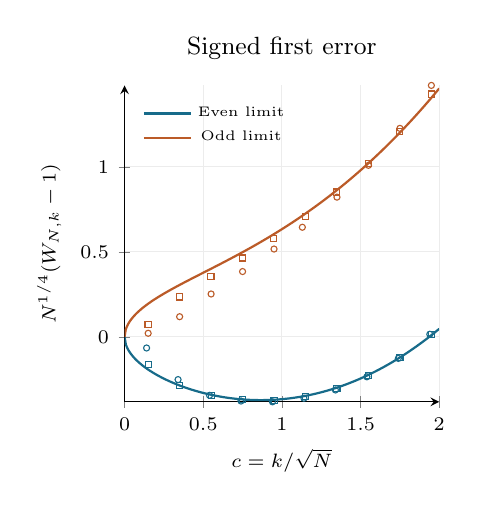
\begin{tikzpicture}
\begin{axis}[width=.46\textwidth,height=5.6cm,xlabel={$c=k/\sqrt N$},ylabel={$N^{1/4}(W_{N,k}-1)$},title={Signed first error},xmin=0,xmax=2,axis lines=left,grid=major,grid style={gray!15},tick label style={font=\scriptsize},label style={font=\scriptsize},title style={font=\small},legend style={font=\tiny,draw=none,fill=none},legend pos=north west,unbounded coords=jump]
\addplot[draw=proofblue,thick] coordinates {(0,0) (0.00803212851406,-0.0448103005641) (0.0160642570281,-0.0633680640097) (0.0240963855422,-0.0776030349499) (0.0321285140562,-0.0895974732062) (0.0401606425703,-0.100157505669) (0.0481927710843,-0.109696278061) (0.0562248995984,-0.118459006299) (0.0642570281124,-0.126605296736) (0.0722891566265,-0.134245878317) (0.0803212851406,-0.141461260613) (0.0883534136546,-0.148312127157) (0.0963855421687,-0.154845541277) (0.104417670683,-0.161098858466) (0.112449799197,-0.16710230317) (0.120481927711,-0.172880728202) (0.128514056225,-0.178454852911) (0.136546184739,-0.183842157237) (0.144578313253,-0.189057541761) (0.152610441767,-0.194113824495) (0.160642570281,-0.199022121197) (0.168674698795,-0.203792140939) (0.176706827309,-0.208432418899) (0.184738955823,-0.212950501954) (0.192771084337,-0.217353098249) (0.200803212851,-0.221646198939) (0.208835341365,-0.225835178168) (0.21686746988,-0.229924875867) (0.224899598394,-0.233919666839) (0.232931726908,-0.2378235188) (0.240963855422,-0.241640041471) (0.248995983936,-0.245372528343) (0.25702811245,-0.249023992401) (0.265060240964,-0.25259719685) (0.273092369478,-0.256094681674) (0.281124497992,-0.259518786682) (0.289156626506,-0.262871671604) (0.29718875502,-0.266155333686) (0.305220883534,-0.269371623146) (0.313253012048,-0.272522256804) (0.321285140562,-0.275608830141) (0.329317269076,-0.278632828009) (0.33734939759,-0.281595634157) (0.345381526104,-0.284498539746) (0.353413654618,-0.287342750967) (0.361445783133,-0.290129395882) (0.369477911647,-0.292859530583) (0.377510040161,-0.295534144739) (0.385542168675,-0.298154166625) (0.393574297189,-0.300720467666) (0.401606425703,-0.303233866567) (0.409638554217,-0.305695133077) (0.417670682731,-0.308104991407) (0.425702811245,-0.310464123364) (0.433734939759,-0.312773171208) (0.441767068273,-0.315032740276) (0.449799196787,-0.31724340139) (0.457831325301,-0.319405693064) (0.465863453815,-0.321520123545) (0.473895582329,-0.323587172689) (0.481927710843,-0.325607293694) (0.489959839357,-0.327580914704) (0.497991967871,-0.329508440289) (0.506024096386,-0.331390252824) (0.5140562249,-0.333226713761) (0.522088353414,-0.335018164818) (0.530120481928,-0.33676492908) (0.538152610442,-0.338467312024) (0.546184738956,-0.340125602479) (0.55421686747,-0.341740073517) (0.562248995984,-0.343310983286) (0.570281124498,-0.344838575795) (0.578313253012,-0.346323081638) (0.586345381526,-0.34776471868) (0.59437751004,-0.349163692697) (0.602409638554,-0.350520197981) (0.610441767068,-0.3518344179) (0.618473895582,-0.353106525432) (0.626506024096,-0.354336683662) (0.63453815261,-0.355525046255) (0.642570281124,-0.356671757897) (0.650602409639,-0.357776954711) (0.658634538153,-0.358840764655) (0.666666666667,-0.35986330789) (0.674698795181,-0.360844697136) (0.682730923695,-0.361785037997) (0.690763052209,-0.362684429283) (0.698795180723,-0.363542963302) (0.706827309237,-0.364360726144) (0.714859437751,-0.365137797948) (0.722891566265,-0.365874253154) (0.730923694779,-0.366570160744) (0.738955823293,-0.367225584472) (0.746987951807,-0.367840583077) (0.755020080321,-0.368415210491) (0.763052208835,-0.368949516034) (0.771084337349,-0.369443544602) (0.779116465863,-0.369897336842) (0.787148594378,-0.370310929322) (0.795180722892,-0.370684354691) (0.803212851406,-0.371017641835) (0.81124497992,-0.371310816018) (0.819277108434,-0.371563899027) (0.827309236948,-0.371776909303) (0.835341365462,-0.371949862067) (0.843373493976,-0.372082769441) (0.85140562249,-0.372175640568) (0.859437751004,-0.37222848172) (0.867469879518,-0.372241296402) (0.875502008032,-0.372214085459) (0.883534136546,-0.372146847168) (0.89156626506,-0.372039577336) (0.899598393574,-0.371892269384) (0.907630522088,-0.371704914435) (0.915662650602,-0.371477501397) (0.923694779116,-0.371210017039) (0.931726907631,-0.370902446068) (0.939759036145,-0.370554771202) (0.947791164659,-0.370166973236) (0.955823293173,-0.369739031111) (0.963855421687,-0.369270921979) (0.971887550201,-0.368762621263) (0.979919678715,-0.368214102714) (0.987951807229,-0.367625338472) (0.995983935743,-0.366996299118) (1.00401606426,-0.366326953726) (1.01204819277,-0.365617269914) (1.02008032129,-0.364867213896) (1.0281124498,-0.364076750523) (1.03614457831,-0.363245843331) (1.04417670683,-0.362374454586) (1.05220883534,-0.361462545321) (1.06024096386,-0.360510075383) (1.06827309237,-0.359517003465) (1.07630522088,-0.358483287148) (1.0843373494,-0.357408882935) (1.09236947791,-0.356293746288) (1.10040160643,-0.355137831657) (1.10843373494,-0.353941092519) (1.11646586345,-0.352703481403) (1.12449799197,-0.351424949924) (1.13253012048,-0.35010544881) (1.140562249,-0.348744927933) (1.14859437751,-0.347343336334) (1.15662650602,-0.345900622248) (1.16465863454,-0.344416733133) (1.17269076305,-0.342891615692) (1.18072289157,-0.341325215898) (1.18875502008,-0.339717479015) (1.19678714859,-0.338068349624) (1.20481927711,-0.336377771638) (1.21285140562,-0.334645688332) (1.22088353414,-0.332872042354) (1.22891566265,-0.33105677575) (1.23694779116,-0.329199829981) (1.24497991968,-0.327301145942) (1.25301204819,-0.325360663979) (1.26104417671,-0.323378323906) (1.26907630522,-0.321354065022) (1.27710843373,-0.319287826126) (1.28514056225,-0.317179545536) (1.29317269076,-0.315029161099) (1.30120481928,-0.312836610209) (1.30923694779,-0.310601829821) (1.31726907631,-0.308324756464) (1.32530120482,-0.306005326254) (1.33333333333,-0.303643474907) (1.34136546185,-0.301239137753) (1.34939759036,-0.298792249746) (1.35742971888,-0.296302745477) (1.36546184739,-0.293770559186) (1.3734939759,-0.291195624772) (1.38152610442,-0.288577875805) (1.38955823293,-0.285917245533) (1.39759036145,-0.283213666897) (1.40562248996,-0.28046707254) (1.41365461847,-0.277677394812) (1.42168674699,-0.274844565785) (1.4297188755,-0.271968517259) (1.43775100402,-0.269049180772) (1.44578313253,-0.266086487606) (1.45381526104,-0.263080368799) (1.46184738956,-0.260030755151) (1.46987951807,-0.256937577233) (1.47791164659,-0.253800765392) (1.4859437751,-0.250620249761) (1.49397590361,-0.247395960266) (1.50200803213,-0.244127826631) (1.51004016064,-0.240815778388) (1.51807228916,-0.23745974488) (1.52610441767,-0.234059655271) (1.53413654618,-0.230615438549) (1.5421686747,-0.227127023535) (1.55020080321,-0.223594338885) (1.55823293173,-0.220017313101) (1.56626506024,-0.216395874533) (1.57429718876,-0.212729951385) (1.58232931727,-0.209019471721) (1.59036144578,-0.20526436347) (1.5983935743,-0.201464554431) (1.60642570281,-0.197619972276) (1.61445783133,-0.193730544558) (1.62248995984,-0.189796198716) (1.63052208835,-0.185816862074) (1.63855421687,-0.181792461852) (1.64658634538,-0.177722925166) (1.6546184739,-0.173608179033) (1.66265060241,-0.169448150378) (1.67068273092,-0.165242766034) (1.67871485944,-0.160991952747) (1.68674698795,-0.15669563718) (1.69477911647,-0.15235374592) (1.70281124498,-0.147966205474) (1.71084337349,-0.143532942281) (1.71887550201,-0.139053882708) (1.72690763052,-0.134528953058) (1.73493975904,-0.129958079573) (1.74297188755,-0.125341188434) (1.75100401606,-0.120678205767) (1.75903614458,-0.115969057645) (1.76706827309,-0.11121367009) (1.77510040161,-0.106411969078) (1.78313253012,-0.10156388054) (1.79116465863,-0.0966693303647) (1.79919678715,-0.0917282444024) (1.80722891566,-0.0867405484662) (1.81526104418,-0.081706168335) (1.82329317269,-0.0766250297563) (1.8313253012,-0.071497058448) (1.83935742972,-0.0663221801008) (1.84738955823,-0.061100320381) (1.85542168675,-0.0558314049319) (1.86345381526,-0.0505153593765) (1.87148594378,-0.0451521093193) (1.87951807229,-0.0397415803487) (1.8875502008,-0.0342836980384) (1.89558232932,-0.0287783879499) (1.90361445783,-0.023225575634) (1.91164658635,-0.0176251866329) (1.91967871486,-0.0119771464818) (1.92771084337,-0.00628138071087) (1.93574297189,-0.00053781484674) (1.9437751004,0.00525362558574) (1.95180722892,0.0110930150618) (1.95983935743,0.0169804280554) (1.96787148594,0.0229159390374) (1.97590361446,0.0288996224742) (1.98393574297,0.0349315528261) (1.99196787149,0.0410118045464) (2,0.0471404520791)};
\addlegendentry{Even limit}
\addplot[draw=prooforange,thick] coordinates {(0,0) (0.00803212851406,0.0448118424256) (0.0160642570281,0.0633767860952) (0.0240963855422,0.0776270701914) (0.0321285140562,0.089646812773) (0.0401606425703,0.100243698345) (0.0481927710843,0.109832241919) (0.0562248995984,0.118658896016) (0.0642570281124,0.126884403474) (0.0722891566265,0.134620550652) (0.0803212851406,0.141948840019) (0.0883534136546,0.148930894047) (0.0963855421687,0.155614669006) (0.104417670683,0.162038373501) (0.112449799197,0.168233050166) (0.120481927711,0.174224339049) (0.128514056225,0.180033719048) (0.136546184739,0.185679404703) (0.144578313253,0.191177008553) (0.152610441767,0.196540039901) (0.160642570281,0.201780286831) (0.168674698795,0.206908113255) (0.176706827309,0.211932693009) (0.184738955823,0.216862196583) (0.192771084337,0.221703941709) (0.200803212851,0.226464516009) (0.208835341365,0.231149877786) (0.21686746988,0.235765439556) (0.224899598394,0.240316137792) (0.232931726908,0.244806491568) (0.240963855422,0.249240652202) (0.248995983936,0.253622445515) (0.25702811245,0.257955408019) (0.265060240964,0.262242818071) (0.273092369478,0.266487722811) (0.281124497992,0.270692961578) (0.289156626506,0.274861186334) (0.29718875502,0.278994879576) (0.305220883534,0.283096370075) (0.313253012048,0.287167846779) (0.321285140562,0.291211371124) (0.329317269076,0.295228887979) (0.33734939759,0.299222235395) (0.345381526104,0.303193153325) (0.353413654618,0.307143291442) (0.361445783133,0.31107421616) (0.369477911647,0.314987416968) (0.377510040161,0.318884312145) (0.385542168675,0.32276625394) (0.393574297189,0.326634533262) (0.401606425703,0.330490383958) (0.409638554217,0.334334986697) (0.417670682731,0.338169472525) (0.425702811245,0.341994926114) (0.433734939759,0.34581238873) (0.441767068273,0.349622860974) (0.449799196787,0.353427305282) (0.457831325301,0.357226648242) (0.465863453815,0.361021782726) (0.473895582329,0.364813569851) (0.481927710843,0.368602840806) (0.489959839357,0.372390398535) (0.497991967871,0.376177019297) (0.506024096386,0.379963454122) (0.5140562249,0.383750430156) (0.522088353414,0.387538651919) (0.530120481928,0.391328802474) (0.538152610442,0.395121544517) (0.546184738956,0.398917521402) (0.55421686747,0.402717358087) (0.562248995984,0.406521662031) (0.570281124498,0.410331024028) (0.578313253012,0.414146018991) (0.586345381526,0.417967206687) (0.59437751004,0.421795132429) (0.602409638554,0.425630327725) (0.610441767068,0.42947331089) (0.618473895582,0.433324587624) (0.626506024096,0.43718465155) (0.63453815261,0.441053984733) (0.642570281124,0.44493305816) (0.650602409639,0.448822332196) (0.658634538153,0.452722257022) (0.666666666667,0.456633273037) (0.674698795181,0.460555811252) (0.682730923695,0.464490293653) (0.690763052209,0.468437133551) (0.698795180723,0.472396735912) (0.706827309237,0.476369497671) (0.714859437751,0.480355808031) (0.722891566265,0.484356048744) (0.730923694779,0.488370594384) (0.738955823293,0.492399812601) (0.746987951807,0.496444064367) (0.755020080321,0.500503704208) (0.763052208835,0.504579080427) (0.771084337349,0.508670535315) (0.779116465863,0.512778405355) (0.787148594378,0.516903021412) (0.795180722892,0.521044708921) (0.803212851406,0.525203788062) (0.81124497992,0.529380573926) (0.819277108434,0.533575376683) (0.827309236948,0.53778850173) (0.835341365462,0.542020249842) (0.843373493976,0.546270917314) (0.85140562249,0.550540796096) (0.859437751004,0.554830173924) (0.867469879518,0.559139334446) (0.875502008032,0.563468557338) (0.883534136546,0.567818118427) (0.89156626506,0.572188289791) (0.899598393574,0.576579339877) (0.907630522088,0.580991533595) (0.915662650602,0.585425132419) (0.923694779116,0.589880394482) (0.931726907631,0.594357574667) (0.939759036145,0.598856924697) (0.947791164659,0.603378693212) (0.955823293173,0.60792312586) (0.963855421687,0.612490465368) (0.971887550201,0.617080951623) (0.979919678715,0.62169482174) (0.987951807229,0.626332310137) (0.995983935743,0.630993648599) (1.00401606426,0.635679066345) (1.01204819277,0.640388790093) (1.02008032129,0.645123044119) (1.0281124498,0.649882050316) (1.03614457831,0.654666028254) (1.04417670683,0.65947519523) (1.05220883534,0.664309766326) (1.06024096386,0.669169954459) (1.06827309237,0.674055970432) (1.07630522088,0.678968022979) (1.0843373494,0.683906318816) (1.09236947791,0.688871062683) (1.10040160643,0.693862457392) (1.10843373494,0.698880703864) (1.11646586345,0.703926001175) (1.12449799197,0.708998546595) (1.13253012048,0.714098535623) (1.140562249,0.719226162029) (1.14859437751,0.724381617892) (1.15662650602,0.729565093628) (1.16465863454,0.734776778031) (1.17269076305,0.740016858304) (1.18072289157,0.745285520091) (1.18875502008,0.75058294751) (1.19678714859,0.755909323181) (1.20481927711,0.761264828259) (1.21285140562,0.766649642459) (1.22088353414,0.772063944089) (1.22891566265,0.777507910072) (1.23694779116,0.782981715975) (1.24497991968,0.788485536035) (1.25301204819,0.794019543186) (1.26104417671,0.799583909077) (1.26907630522,0.805178804104) (1.27710843373,0.810804397427) (1.28514056225,0.816460856995) (1.29317269076,0.822148349567) (1.30120481928,0.827867040735) (1.30923694779,0.833617094944) (1.31726907631,0.839398675511) (1.32530120482,0.845211944646) (1.33333333333,0.851057063472) (1.34136546185,0.856934192042) (1.34939759036,0.862843489357) (1.35742971888,0.868785113388) (1.36546184739,0.874759221089) (1.3734939759,0.880765968414) (1.38152610442,0.886805510337) (1.38955823293,0.892878000866) (1.39759036145,0.898983593058) (1.40562248996,0.905122439037) (1.41365461847,0.911294690005) (1.42168674699,0.917500496262) (1.4297188755,0.923740007215) (1.43775100402,0.930013371398) (1.44578313253,0.936320736478) (1.45381526104,0.942662249277) (1.46184738956,0.949038055776) (1.46987951807,0.955448301137) (1.47791164659,0.961893129709) (1.4859437751,0.968372685042) (1.49397590361,0.9748871099) (1.50200803213,0.981436546272) (1.51004016064,0.988021135382) (1.51807228916,0.994641017702) (1.52610441767,1.00129633296) (1.53413654618,1.00798722017) (1.5421686747,1.0147138176) (1.55020080321,1.02147626281) (1.55823293173,1.02827469269) (1.56626506024,1.03510924341) (1.57429718876,1.04198005047) (1.58232931727,1.0488872487) (1.59036144578,1.05583097225) (1.5983935743,1.06281135466) (1.60642570281,1.06982852877) (1.61445783133,1.07688262684) (1.62248995984,1.08397378046) (1.63052208835,1.09110212062) (1.63855421687,1.09826777769) (1.64658634538,1.10547088147) (1.6546184739,1.11271156112) (1.66265060241,1.11998994523) (1.67068273092,1.12730616183) (1.67871485944,1.13466033836) (1.68674698795,1.14205260168) (1.69477911647,1.14948307814) (1.70281124498,1.15695189348) (1.71084337349,1.16445917295) (1.71887550201,1.17200504122) (1.72690763052,1.17958962246) (1.73493975904,1.1872130403) (1.74297188755,1.19487541787) (1.75100401606,1.20257687775) (1.75903614458,1.21031754207) (1.76706827309,1.21809753241) (1.77510040161,1.22591696989) (1.78313253012,1.23377597512) (1.79116465863,1.24167466825) (1.79919678715,1.24961316894) (1.80722891566,1.25759159638) (1.81526104418,1.26561006929) (1.82329317269,1.27366870595) (1.8313253012,1.28176762416) (1.83935742972,1.28990694129) (1.84738955823,1.29808677426) (1.85542168675,1.30630723953) (1.86345381526,1.31456845316) (1.87148594378,1.32287053076) (1.87951807229,1.33121358751) (1.8875502008,1.33959773819) (1.89558232932,1.34802309713) (1.90361445783,1.35648977828) (1.91164658635,1.36499789517) (1.91967871486,1.37354756093) (1.92771084337,1.38213888829) (1.93574297189,1.39077198958) (1.9437751004,1.39944697674) (1.95180722892,1.40816396133) (1.95983935743,1.41692305453) (1.96787148594,1.42572436714) (1.97590361446,1.43456800956) (1.98393574297,1.44345409186) (1.99196787149,1.45238272372) (2,1.46135401445)};
\addlegendentry{Odd limit}
\addplot[only marks,mark=o,mark size=1.1pt,draw=proofblue] coordinates {(0.14,-0.0655362703588) (0.34,-0.251485743416) (0.54,-0.344104748785) (0.74,-0.377621096149) (0.94,-0.382308717551) (1.14,-0.360952355623) (1.34,-0.312505985807) (1.54,-0.235206740583) (1.74,-0.126839589284) (1.94,0.0152367293872)};
\addplot[only marks,mark=o,mark size=1.1pt,draw=prooforange] coordinates {(0.15,0.0209949285747) (0.35,0.118555998928) (0.55,0.252084425726) (0.75,0.384111660159) (0.95,0.516434410597) (1.13,0.644626050014) (1.35,0.82184712535) (1.55,1.00895858166) (1.75,1.2263120504) (1.95,1.47901688188)};
\addplot[only marks,mark=square,mark size=1.1pt,draw=proofblue] coordinates {(0.15,-0.162801661892) (0.35,-0.287666822492) (0.55,-0.343191808164) (0.75,-0.37094449156) (0.95,-0.373343028395) (1.15,-0.350473562924) (1.35,-0.301576619559) (1.55,-0.225493031674) (1.75,-0.120835905589) (1.95,0.0139381089318)};
\addplot[only marks,mark=square,mark size=1.1pt,draw=prooforange] coordinates {(0.149,0.0707317236727) (0.349,0.234571365473) (0.549,0.354492573771) (0.749,0.463786593012) (0.949,0.57852193049) (1.149,0.706192810475) (1.349,0.851590595576) (1.549,1.01837249397) (1.749,1.20964127187) (1.949,1.42821232427)};
\end{axis}
\end{tikzpicture}\hfill
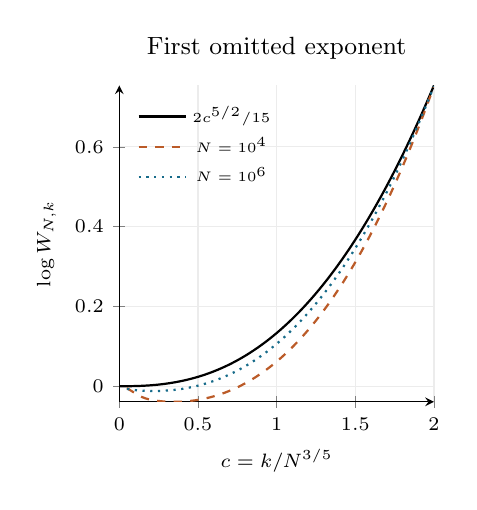
\begin{tikzpicture}
\begin{axis}[width=.46\textwidth,height=5.6cm,xlabel={$c=k/N^{3/5}$},ylabel={$\log W_{N,k}$},title={First omitted exponent},xmin=0,xmax=2,axis lines=left,grid=major,grid style={gray!15},tick label style={font=\scriptsize},label style={font=\scriptsize},title style={font=\small},legend style={font=\tiny,draw=none,fill=none},legend pos=north west,unbounded coords=jump]
\addplot[black,thick] coordinates {(0,0) (0.00803212851406,7.70930731136e-07) (0.0160642570281,4.36104278249e-06) (0.0240963855422,1.2017620759e-05) (0.0321285140562,2.46697833963e-05) (0.0401606425703,4.30963380191e-05) (0.0481927710843,6.79819290593e-05) (0.0562248995984,9.99448586395e-05) (0.0642570281124,0.00013955336904) (0.0722891566265,0.000187336167666) (0.0803212851406,0.000243789702861) (0.0883534136546,0.000309383444918) (0.0963855421687,0.000384563864288) (0.104417670683,0.000469757517479) (0.112449799197,0.00056537349831) (0.120481927711,0.000671805423623) (0.128514056225,0.000789433068683) (0.136546184739,0.000918623733173) (0.144578313253,0.00105973339614) (0.152610441767,0.00121310770297) (0.160642570281,0.00137908281661) (0.168674698795,0.00155798615807) (0.176706827309,0.00175013705511) (0.184738955823,0.00195584731451) (0.192771084337,0.0021754217299) (0.200803212851,0.0024091585348) (0.208835341365,0.00265734980898) (0.21686746988,0.00292028184443) (0.224899598394,0.00319823547646) (0.232931726908,0.00349148638436) (0.240963855422,0.00380030536545) (0.248995983936,0.00412495858564) (0.25702811245,0.00446570780927) (0.265060240964,0.00482281061057) (0.273092369478,0.00519652056868) (0.281124497992,0.00558708744799) (0.289156626506,0.00599475736531) (0.29718875502,0.00641977294522) (0.305220883534,0.00686237346462) (0.313253012048,0.0073227949876) (0.321285140562,0.00780127049154) (0.329317269076,0.00829802998511) (0.33734939759,0.00881330061893) (0.345381526104,0.00934730678957) (0.353413654618,0.00990027023739) (0.361445783133,0.0104724101386) (0.369477911647,0.0110639431925) (0.377510040161,0.011675083703) (0.385542168675,0.0123060436572) (0.393574297189,0.0129570327982) (0.401606425703,0.0136282586953) (0.409638554217,0.01431992681) (0.417670682731,0.0150322405593) (0.425702811245,0.0157654013751) (0.433734939759,0.0165196087614) (0.441767068273,0.0172950603488) (0.449799196787,0.0180919519459) (0.457831325301,0.0189104775893) (0.465863453815,0.0197508295904) (0.473895582329,0.0206131985809) (0.481927710843,0.0214977735559) (0.489959839357,0.0224047419154) (0.497991967871,0.0233342895041) (0.506024096386,0.0242866006494) (0.5140562249,0.0252618581979) (0.522088353414,0.0262602435506) (0.530120481928,0.0272819366969) (0.538152610442,0.0283271162466) (0.546184738956,0.0293959594615) (0.55421686747,0.0304886422853) (0.562248995984,0.0316053393724) (0.570281124498,0.0327462241165) (0.578313253012,0.0339114686766) (0.586345381526,0.0351012440039) (0.59437751004,0.036315719866) (0.602409638554,0.0375550648718) (0.610441767068,0.0388194464949) (0.618473895582,0.0401090310957) (0.626506024096,0.0414239839438) (0.63453815261,0.0427644692389) (0.642570281124,0.0441306501315) (0.650602409639,0.0455226887428) (0.658634538153,0.0469407461837) (0.666666666667,0.0483849825735) (0.674698795181,0.0498555570582) (0.682730923695,0.051352627828) (0.690763052209,0.0528763521339) (0.698795180723,0.0544268863049) (0.706827309237,0.0560043857635) (0.714859437751,0.0576090050415) (0.722891566265,0.0592408977952) (0.730923694779,0.0609002168199) (0.738955823293,0.0625871140644) (0.746987951807,0.064301740645) (0.755020080321,0.0660442468586) (0.763052208835,0.0678147821965) (0.771084337349,0.0696134953567) (0.779116465863,0.0714405342566) (0.787148594378,0.0732960460453) (0.795180722892,0.0751801771151) (0.803212851406,0.0770930731136) (0.81124497992,0.0790348789542) (0.819277108434,0.0810057388278) (0.827309236948,0.0830057962132) (0.835341365462,0.0850351938874) (0.843373493976,0.0870940739362) (0.85140562249,0.0891825777636) (0.859437751004,0.0913008461022) (0.867469879518,0.0934490190219) (0.875502008032,0.0956272359398) (0.883534136546,0.0978356356291) (0.89156626506,0.100074356228) (0.899598393574,0.102343535247) (0.907630522088,0.10464330958) (0.915662650602,0.106973815511) (0.923694779116,0.109335188722) (0.931726907631,0.1117275643) (0.939759036145,0.114151076747) (0.947791164659,0.116605859988) (0.955823293173,0.119092047374) (0.963855421687,0.121609771694) (0.971887550201,0.12415916518) (0.979919678715,0.126740359513) (0.987951807229,0.129353485832) (0.995983935743,0.13199867474) (1.00401606426,0.13467605631) (1.01204819277,0.137385760089) (1.02008032129,0.140127915111) (1.0281124498,0.142902649897) (1.03614457831,0.145710092461) (1.04417670683,0.148550370322) (1.05220883534,0.151423610502) (1.06024096386,0.154329939538) (1.06827309237,0.157269483484) (1.07630522088,0.160242367916) (1.0843373494,0.16324871794) (1.09236947791,0.166288658198) (1.10040160643,0.169362312867) (1.10843373494,0.172469805673) (1.11646586345,0.175611259886) (1.12449799197,0.178786798336) (1.13253012048,0.181996543406) (1.140562249,0.185240617048) (1.14859437751,0.188519140779) (1.15662650602,0.19183223569) (1.16465863454,0.195180022449) (1.17269076305,0.198562621306) (1.18072289157,0.201980152096) (1.18875502008,0.205432734247) (1.19678714859,0.208920486779) (1.20481927711,0.21244352831) (1.21285140562,0.216001977064) (1.22088353414,0.219595950868) (1.22891566265,0.223225567161) (1.23694779116,0.226890942997) (1.24497991968,0.230592195046) (1.25301204819,0.234329439603) (1.26104417671,0.238102792586) (1.26907630522,0.241912369541) (1.27710843373,0.24575828565) (1.28514056225,0.249640655729) (1.29317269076,0.253559594234) (1.30120481928,0.257515215263) (1.30923694779,0.261507632562) (1.31726907631,0.265536959524) (1.32530120482,0.269603309196) (1.33333333333,0.273706794282) (1.34136546185,0.277847527144) (1.34939759036,0.282025619806) (1.35742971888,0.286241183956) (1.36546184739,0.290494330951) (1.3734939759,0.294785171821) (1.38152610442,0.299113817266) (1.38955823293,0.303480377667) (1.39759036145,0.30788496308) (1.40562248996,0.312327683248) (1.41365461847,0.316808647596) (1.42168674699,0.321327965238) (1.4297188755,0.325885744978) (1.43775100402,0.330482095313) (1.44578313253,0.335117124436) (1.45381526104,0.339790940239) (1.46184738956,0.344503650312) (1.46987951807,0.349255361952) (1.47791164659,0.354046182159) (1.4859437751,0.358876217641) (1.49397590361,0.363745574817) (1.50200803213,0.36865435982) (1.51004016064,0.373602678497) (1.51807228916,0.378590636411) (1.52610441767,0.383618338847) (1.53413654618,0.38868589081) (1.5421686747,0.393793397031) (1.55020080321,0.398940961964) (1.55823293173,0.404128689796) (1.56626506024,0.409356684439) (1.57429718876,0.414625049542) (1.58232931727,0.419933888487) (1.59036144578,0.425283304391) (1.5983935743,0.430673400113) (1.60642570281,0.436104278249) (1.61445783133,0.44157604114) (1.62248995984,0.44708879087) (1.63052208835,0.452642629271) (1.63855421687,0.458237657921) (1.64658634538,0.463873978151) (1.6546184739,0.469551691041) (1.66265060241,0.475270897427) (1.67068273092,0.481031697898) (1.67871485944,0.486834192804) (1.68674698795,0.492678482252) (1.69477911647,0.498564666108) (1.70281124498,0.504492844003) (1.71084337349,0.510463115332) (1.71887550201,0.516475579255) (1.72690763052,0.522530334701) (1.73493975904,0.528627480365) (1.74297188755,0.534767114716) (1.75100401606,0.540949335994) (1.75903614458,0.547174242212) (1.76706827309,0.55344193116) (1.77510040161,0.559752500405) (1.78313253012,0.566106047291) (1.79116465863,0.572502668944) (1.79919678715,0.578942462269) (1.80722891566,0.585425523956) (1.81526104418,0.591951950479) (1.82329317269,0.598521838097) (1.8313253012,0.605135282858) (1.83935742972,0.611792380596) (1.84738955823,0.618493226938) (1.85542168675,0.625237917301) (1.86345381526,0.632026546894) (1.87148594378,0.638859210721) (1.87951807229,0.645736003583) (1.8875502008,0.652657020074) (1.89558232932,0.65962235459) (1.90361445783,0.666632101324) (1.91164658635,0.673686354271) (1.91967871486,0.680785207226) (1.92771084337,0.68792875379) (1.93574297189,0.695117087365) (1.9437751004,0.702350301163) (1.95180722892,0.709628488198) (1.95983935743,0.716951741294) (1.96787148594,0.724320153087) (1.97590361446,0.731733816018) (1.98393574297,0.739192822344) (1.99196787149,0.746697264133) (2,0.754247233266)};
\addlegendentry{$2c^{5/2}/15$}
\addplot[draw=prooforange,thick,dashed] coordinates {(0.0477728604664,-0.00493909415142) (0.0636971472886,-0.00837819447345) (0.0875835775218,-0.0143771044526) (0.103507864344,-0.0184322241542) (0.127394294577,-0.0238937702399) (0.143318581399,-0.0269134362292) (0.167205011632,-0.0304829367528) (0.183129298455,-0.0323143686097) (0.207015728688,-0.034438968288) (0.22294001551,-0.0355403708645) (0.246826445743,-0.0368411694784) (0.262750732565,-0.0375185541877) (0.278675019387,-0.0380658000816) (0.302561449621,-0.03866472778) (0.318485736443,-0.0389240638285) (0.342372166676,-0.0391095344563) (0.358296453498,-0.0390988467075) (0.382182883731,-0.038881517183) (0.398107170553,-0.038601863803) (0.421993600787,-0.0379786018017) (0.437917887609,-0.0374260464668) (0.461804317842,-0.0363893239456) (0.477728604664,-0.0355581121666) (0.501615034897,-0.0340985244621) (0.51753932172,-0.0329819865431) (0.541425751953,-0.0310890614243) (0.557350038775,-0.0296799597947) (0.581236469008,-0.0273425305968) (0.59716075583,-0.0256332483758) (0.621047186063,-0.0228396795109) (0.636971472886,-0.0208223428496) (0.652895759708,-0.0186795388875) (0.676782189941,-0.0152272445144) (0.692706476763,-0.012765087083) (0.716592906996,-0.00882763191057) (0.732517193818,-0.0060379299711) (0.756403624052,-0.00160297997452) (0.772327910874,0.00152251332688) (0.796214341107,0.00646735373379) (0.812138627929,0.00993691352966) (0.836025058162,0.0154040661363) (0.851949344984,0.0192259756716) (0.875835775218,0.0252278625299) (0.89176006204,0.0294103983502) (0.915646492273,0.035959422717) (0.931570779095,0.0405108437925) (0.955457209328,0.0476193761563) (0.971381496151,0.0525479159278) (0.995267926384,0.0602282838283) (1.01119221321,0.0655421444417) (1.02711650003,0.0710124221685) (1.05100293026,0.0795139733298) (1.06692721708,0.0853809947368) (1.09081364732,0.0944837528605) (1.10673793414,0.10075563052) (1.13062436437,0.110471734131) (1.14654865119,0.117156539884) (1.17043508143,0.127498065608) (1.18635936825,0.134603829624) (1.21024579848,0.145582791177) (1.2261700853,0.153117501524) (1.25005651554,0.164745849369) (1.26598080236,0.172717451957) (1.28986723259,0.185007073462) (1.30579151942,0.193423472288) (1.32967794965,0.206386192268) (1.34560223647,0.215255249886) (1.3694886667,0.228902831441) (1.38541295353,0.238232369597) (1.40133724035,0.247748281058) (1.42522367058,0.262374315561) (1.4411479574,0.272361590915) (1.46503438764,0.287700473288) (1.48095867446,0.298166839623) (1.50484510469,0.314230131916) (1.52076939151,0.325183278437) (1.54465582175,0.341982486602) (1.56058010857,0.353430065606) (1.5844665388,0.37097664099) (1.60039082563,0.382926268878) (1.62427725586,0.401231609744) (1.64020154268,0.413690868037) (1.66408797291,0.432766321091) (1.68001225974,0.445742757449) (1.70389868997,0.465599619375) (1.71982297679,0.479100748619) (1.74370940702,0.499750267597) (1.75963369385,0.513783572715) (1.77555798067,0.528031836477) (1.7994444109,0.549809883069) (1.81536869772,0.564600747303) (1.83925512796,0.587198257641) (1.85517941478,0.602539132967) (1.87906584501,0.625967201428) (1.89499013183,0.641865469949) (1.91887656207,0.666135148837) (1.93480084889,0.682598165068) (1.95868727912,0.707720465988) (1.97461156595,0.724755557766) (1.99849799618,0.750741452977)};
\addlegendentry{$N=10^4$}
\addplot[draw=proofblue,thick,dotted] coordinates {(0.0497353513439,-0.00668789854734) (0.0693280655097,-0.00817845230437) (0.0889207796754,-0.0091841952666) (0.109015871128,-0.0100031887764) (0.128608585293,-0.0106479115864) (0.148201299459,-0.0111561573387) (0.167794013625,-0.0115354504236) (0.187386727791,-0.0117899087236) (0.207481819243,-0.0119233584293) (0.227074533408,-0.0119298421429) (0.246667247574,-0.0118140511279) (0.26625996174,-0.0115751477199) (0.286355053192,-0.0112008869555) (0.305947767358,-0.0107083449733) (0.325540481524,-0.0100879301182) (0.345133195689,-0.00933763698186) (0.364725909855,-0.00845533600048) (0.384821001307,-0.00741095650641) (0.404413715473,-0.00625438080593) (0.424006429639,-0.00495889510482) (0.443599143805,-0.00352213131787) (0.46319185797,-0.00194169962473) (0.483286949422,-0.00016898561415) (0.502879663588,0.0017098363175) (0.522472377754,0.00373961128803) (0.54206509192,0.00592274718613) (0.561657806086,0.00826164580146) (0.581752897538,0.0108248281613) (0.601345611703,0.0134865687677) (0.620938325869,0.0163112789774) (0.640531040035,0.0193013156373) (0.660123754201,0.0224590213772) (0.680218845653,0.0258743055359) (0.699811559819,0.0293787657172) (0.719404273984,0.0330578903728) (0.73899698815,0.036913959757) (0.758589702316,0.0409492380329) (0.778684793768,0.0452765005094) (0.798277507934,0.04968166368) (0.8178702221,0.0542727880919) (0.837462936265,0.0590520732071) (0.857558027717,0.0641516512337) (0.877150741883,0.0693187576229) (0.896743456049,0.0746805838744) (0.916336170215,0.0802392668656) (0.93592888438,0.0859969284324) (0.956023975833,0.0921111267151) (0.975616689998,0.0982782889832) (0.995209404164,0.10465076046) (1.01480211833,0.111230604761) (1.0343948325,0.118019871634) (1.05448992395,0.1252029015) (1.07408263811,0.132422608877) (1.09367535228,0.139857858649) (1.11326806645,0.147510647172) (1.13286078061,0.155382958134) (1.15295587206,0.163687226125) (1.17254858623,0.17201023869) (1.19214130039,0.180558700772) (1.21173401456,0.18933454733) (1.23132672873,0.198339701772) (1.25142182018,0.207815963539) (1.27101453434,0.217291461145) (1.29060724851,0.227002017915) (1.31019996268,0.236949512815) (1.33029505413,0.247400158126) (1.34988776829,0.257833319416) (1.36948048246,0.268509040456) (1.38907319662,0.279429158884) (1.40866591079,0.290595502524) (1.42876100224,0.302305843808) (1.44835371641,0.313976513094) (1.46794643057,0.325898879875) (1.48753914474,0.338074734146) (1.50713185891,0.350505856908) (1.52722695036,0.363522753402) (1.54681966452,0.37647638002) (1.56641237869,0.389690610524) (1.58600509286,0.403167191188) (1.60559780702,0.416907860012) (1.62569289847,0.431276998158) (1.64528561264,0.44555790745) (1.6648783268,0.460108114441) (1.68447104097,0.474929325152) (1.70406375514,0.490023237976) (1.72415884659,0.50578922594) (1.74375156075,0.521440709191) (1.76334427492,0.537369988009) (1.78293698909,0.553578731244) (1.80252970325,0.570068600685) (1.8226247947,0.587275052134) (1.84221750887,0.604339446308) (1.86181022303,0.621689952739) (1.8814029372,0.639328205844) (1.90149802865,0.657719335712) (1.92109074282,0.675945441993) (1.94068345698,0.694464200586) (1.96027617115,0.713277220096) (1.97986888532,0.732386102944) (1.99996397677,0.752293969482)};
\addlegendentry{$N=10^6$}
\end{axis}
\end{tikzpicture}
\caption{Two views of the next error. Left: the signed functions $\psi_0(c)$ and $\psi_1(c)$, compared with the positive recurrence at $N=10^4$ and $10^6$. Right: $\log W_{N,k}$ at $k\sim cN^{3/5}$ approaches $2c^{5/2}/15$. These finite evaluations corroborate the general theorems and are not used in their proofs.}
\label{fig:ratehierarchy}
\end{figure}


\clearpage
\section{Two checks on a conditioning formula}\label{sec:conditioning}

The following examples concern equation (62) on printed page 1428 of Bordenave's published article \cite{Bordenave}. The same formula appears on page 38 of arXiv version 4. They refute that intermediate conditional assertion under its displayed conditioning. They are not counterexamples to Proposition 28, which appears on printed page 1426 and which Section~\ref{sec:mixed} proves by a different argument.

For requested cells $y_t=(i_t,j_t)$, the source conditions on
\[
\mathcal F_t=\sigma\bigl(\sigma(i_s),\sigma^{-1}(j_s):s\ne t\bigr)
\]
and asserts a probability of the form
\[
\PP(M_{i_tj_t}=1\mid\mathcal F_t)
=\frac{\1_{\Omega_t^c}}{n_t}\le\frac1{n-a+1},
\qquad
n_t=n-|\{\sigma(i_s):s\ne t\}|.
\]
The event $\Omega_t$ holds if some $s\ne t$ satisfies $\sigma(i_s)=j_t$ or $\sigma^{-1}(j_s)=i_t$.

\begin{example}[A shared row reveals the cell]
Let $n=4$, $y_1=(1,1)$ and $y_2=(1,2)$. Then $a=k=2\le\sqrt n$, and $\mathcal F_1$ includes $\sigma(1)$. On the event $\sigma(1)=1$, of probability $1/4$, the actual conditional probability of $M_{11}=1$ is one. The displayed event $\Omega_1$ also holds, because $\sigma(i_2)=j_1$. The source formula therefore gives zero. Its claimed upper bound $1/3$ fails as well.
\end{example}

\begin{example}[Images and preimages remove two arrows]
Let $n=4$, $y_1=(1,1)$ and $y_2=(2,2)$. Condition on
\[
\sigma(2)=3,\qquad \sigma^{-1}(2)=4.
\]
This event has probability $1/12$. It exposes two arrows, $2\mapsto3$ and $4\mapsto2$. The remaining rows are $1,3$ and the remaining columns are $1,4$. Thus
\[
\PP(M_{11}=1\mid\mathcal F_1)=\frac12.
\]
Neither clause of $\Omega_1$ holds, but the displayed $n_t$ is $4-1=3$. The source formula gives $1/3$, and the proposed bound $1/(n-a+1)$ also gives $1/3$.
\end{example}

The second example shows that merely requiring the tested cell to be unrevealed does not repair the formula. One must count every removed row and column under the actual conditioning. Section~\ref{sec:mixed} avoids the issue by exposing only a compatible prescribed set. Its remaining dimension is exactly $n-r$.


\clearpage
\section{Prior work and limits of the moment refinements}\label{sec:moment-discussion}

The mixed-product theorems identify attained maxima when there are zero, one or two inconsistent centered singletons. Their proofs keep the exact depleted moment, merge colors through positive partition weights, and handle arbitrary multiplicities through affine indicator identities. For one distinguished inconsistent singleton, an exact kernel difference exchanges a missing conflicting neighbor for one extra prescribed match. This also improves the general inconsistent-singleton bound. The scalar consequences recover the spectral estimate with a smaller singleton factor and an optimal universal prefactor. The diagonal results determine the original cubic threshold, the parity transition, a hierarchy of further corrections and sharp first uniform errors for both the square-root and full-range approximations.

The base recurrence, its normalized parity form and the leading coefficients belong to Collins and Nagatsu \cite{CN}. The mixed estimate itself is already part of Bordenave's spectral-gap method \cite{Bordenave}. The special-function identities and the saddle method are classical. The attained envelope at fixed support and singleton counts is the principal finite extremal result. The diagonal theorems give explicit uniform consequences and elementary proofs in the probabilistic normalization, including the necessity and bounded-comparability characterization of the cubic scale. Classical uniform asymptotic theory supplies another route to the corrections. We do not claim a new special-function method or base historical novelty on a mismatch with only one prior parameter regime.

Bordenave and Zhu \cite[Lemma 2.1]{BZ} retain the original singleton factor $3k/\sqrt N$ and explicitly bound the raw factorial ratio by $\sqrt e$ in their equation (2.3). That elementary bound is a known ingredient here. Our exact refinement retains $\mu_h(n,a-h)$ in addition to $F_n(a-h)$. The factor $\Gamma_{n,a,h}$ is a scalar upper bound on that moment and is smaller than $\beta$ when $1\le h<a$. Theorems~\ref{thm:mixed} and \ref{thm:oneconflict} give exact maxima for $b=0$ and $b=1$, respectively. The latter theorem also replaces the general factor $2^bK_{h,a-h}$ by $2^{b-1}K_{h,a-h-1}$. Theorem~\ref{thm:twoconflict} further subtracts a nonnegative kernel term and attains the resulting maximum at $b=2$. No exact maximum is claimed for $b>2$. A same-row clique need not be extremal for larger $b$. At $n=a=b=8$ and $h=0$, use four disjoint rows, each requesting its own two columns, and center all eight cells. Expanding by rows gives
\[
n^8\E P=\sum_{j=0}^4\binom4j(-2)^j\frac{8^j}{(8)_j}
=\frac{1121}{105}>7,
\]
whereas the eight-cell same-row clique has scaled absolute expectation seven.

A nearby fixed-pattern calculation is already explicit in Collins and Nagatsu \cite[Remark 7.2, page 478]{CN}:
\[
\E\bigl[(M_{11}-n^{-1})^2(M_{12}-n^{-1})^2
(M_{13}-n^{-1})(M_{14}-n^{-1})\bigr]
=2n^{-5}-5n^{-6}.
\]
It belongs to the class $a=4,h=0,b=2$. The contribution of Theorem~\ref{thm:twoconflict} is the maximum over all permitted patterns, powers and independent colors, rather than the evaluation of this or another fixed pattern.

The depleted polynomial itself is also a classical specialization. If $d_h^{(r)}(x)$ denotes the higher-order derangement polynomial defined by $(1-t)^{-r}e^{xt}$ in \cite[equation (2.22)]{KKJK}, then
\[
\mathcal P_h(n,s)=(-1)^h d_h^{(n-s-h+1)}(-n).
\]
Indeed, the indicator expansion gives $\mathcal P_h(n,s)=\E(n-V)^h$ for a gamma variable $V$ of shape $n-s-h+1$ and unit scale. Its moment generating function proves the identity. The order is positive on $h+s\le n$ and depends on $h$. Thus neither the polynomial family nor this elementary connection is asserted to be new. The extremal conclusions concern the full class of mixed cell patterns.

Related centered-matrix and permanent inequalities already bound the same diagonal moments. For example, set $B_n=nI-J$, where $J$ is the all-ones matrix. For the matrix elementary symmetric polynomial of Han and Niles-Weed \cite[equation (2), Theorem 1.2]{HNcentered}, summing over injections gives
\[
e_h(B_n)=\binom nh^2\mu_h(n,0),\qquad
\|B_n\|_F=n\sqrt{n-1}.
\]
Their theorem therefore implies
\[
0\le\mu_h(n,0)\le
\frac{(8e^2)^h(n-1)^{h/2}}{\binom nh}\qquad(1\le h\le n).
\]
The permanent expansion in their earlier work \cite[equation (29), Lemma 5.5 in the inspected preprint]{HNmixtures} also contains these moments: the coefficient of $t^h$ in
$n^n\operatorname{Perm}((J+tB_n)/n)/n!$ is $\binom nh\mu_h(n,0)$.
These are genuine overlaps. The inspected statements do not give the exact maximum over our mixed class, whose proof additionally uses positive depletion weights, color merging and attainment.

The Laguerre representation makes the parameter regime precise: the degree is $k$, the parameter is $\alpha=-N-1$, and the argument is $-N$. Thus $-\alpha/k\to\infty$ throughout the sublinear range. Kuijlaars and McLaughlin \cite[Theorem 7.1 and Remark 5.4]{KM}, and the regime announced by Dai and Wong \cite{DW}, treat a finite limiting ratio greater than one. Their parameter ranges overlap the interior proportional-degree part of our full-range formula. Theorem 1 of Dai, Ismail and Wang \cite{DIW} assumes $\alpha>0$ when $\alpha/k\to\infty$. In the inspected preprint of Dunster, Gil and Segura \cite[Section 1, equation (1.6) and Cases 1a, 1b and 2]{DGS}, $\alpha=(k+1/2)(a^2-1)$ with $a\ge0$, excluding $\alpha=-N-1$ for $k\le N$. These comparisons concern those specific statements. They do not exclude other classical uniform expansions.

In particular, the Whittaker connection formulas put the problem at positive argument $N$, with parameters $\kappa=N/2-k$ and $\mu=(N+1)/2$. For every fixed $c<1$, the range $k\le cN$ lies in the uniform domain of Olver's parabolic-cylinder approximations \cite{Olver,DLMFWhittaker}. The odd moment involves a difference of the two solutions, so cancellation must be retained when transporting individual relative errors. There is no parameter-domain obstruction to this route in the sublinear range.

The underlying integral connection can also be checked without special-function notation. Expanding $(N-s)^k$ and integrating each monomial gives the exact identity
\begin{equation}\label{eq:gammaidentity}
Q_k=\frac1{(N-k)!}\int_0^\infty
e^{-s}s^{N-k}(N-s)^k\,ds.
\end{equation}
Indeed, its expansion is
$\sum_{j=0}^k\binom kj(-1)^{k-j}N^j(N-j)!/(N-k)!$,
which is the indicator formula for $Q_k$. Splitting the integral at $N$ and putting $s=N(1\mp t)$ yields
\begin{align*}
Q_k&=\frac{N^{N+1}e^{-N}}{(N-k)!}
\bigl(J_++(-1)^kJ_-\bigr),\\
J_+&=\int_0^1 e^{Nt}t^k(1-t)^{N-k}\,dt,\qquad
J_-=\int_0^\infty e^{-Nt}t^k(1+t)^{N-k}\,dt.
\end{align*}
For $k<N$, both positive integrals have their stationary point at $t=\sqrt{k/N}$. Thus even orders add two contributions and odd orders subtract them. Standard Laplace expansion of this classical representation provides another route to the action and first correction. The positive partition proof used above makes the low-order patch and the explicit error constants transparent.

At $k=N$, the identity with a truncated exponential is classical, as recorded in \cite[Section 1]{DMO}. The contribution of Theorem~\ref{thm:global} is a self-contained formula that patches fixed orders, the parity transition and the endpoint while keeping $(N)_k$ exact. Its optimal global error is $C_*N^{-1/3}+o(N^{-1/3})$. Appendix~\ref{sec:globalsharpproof} gives the full parity profile, controls both tails and proves uniqueness of the limiting maximizing scale. The sharp $N^{-1/4}$ rate in Section~\ref{sec:rates} concerns the different, quartically corrected hyperbolic approximation. These explicit probabilistic refinements are not claimed to be historically independent of classical asymptotic theory.

A bounded source search found no exact duplicate of the attained mixed maximum or the complete collection of uniform probabilistic statements. This is a search outcome, not a priority certificate. Some journal bodies remained inaccessible, as recorded in the accompanying source audit. The elementary integral calculation above is not presented as a newly discovered special-function identity.

The inequalities are proved symbolically for their stated parameter ranges. Exact finite computations check normalization, the depleted recurrence and the conditioning examples. Numerical plots illustrate the asymptotic regimes. Neither kind of computation is used as a substitute for a general proof.

The remaining graph-level task is to combine the sharper cell-pattern estimate with circuit enumeration and tangle remainders while retaining the degree dependence. A better estimate for one fixed product does not automatically improve a spectral theorem: the patterns that dominate the full sum must be identified first. The present paper does not assert a new second-eigenvalue bound or an end-to-end audit of either random-graph proof.


\clearpage
\section{Explicit constants and proof of the uniform rate}\label{sec:rateproof}

We prove Theorem~\ref{thm:rate} without a lower bound on the moment order or the hyperbolic parameter. Throughout this appendix,
\[
m=\lfloor k/2\rfloor,\quad K=2m,\quad\epsilon=k-K,\quad
\lambda=\frac23\sqrt{K^3/N},\quad
\delta=\frac{K^2}{N},\quad\eta=\frac{3K^2}{4N}.
\]
The symbol $\delta$ here denotes the scale parameter, not parity.

\subsection{Constants and a finite estimate}

For $C>0$, put $a=3C^2/4$ and define
\begin{equation}\label{eq:rateconstantsB}
\begin{aligned}
B_1(C)&=\frac43(2+3a)\sqrt C+\frac{2144}{27}C^{5/2},\\
B_2(C)&=\frac32(2a+3)C
+\frac{16}{9}(245+45a+45a^2)C,\\
B_3(C)&=3(10a^3+188a^2+457a+141).
\end{aligned}
\end{equation}
One valid choice in \eqref{eq:ratefinite} is
\begin{equation}\label{eq:rateconstantsA}
\begin{aligned}
A_1(C)&=e^{7C^2/4}B_1(C)+2e^{11C^2/4}C^{5/2},\\
A_2(C)&=e^{7C^2/4}B_2(C)+2e^{11C^2/4}C
+e^{C^2/3}\left(\frac C2+\frac{C^3}{3}\right),\\
A_3(C)&=e^{7C^2/4}B_3(C).
\end{aligned}
\end{equation}
In particular, the displayed expression for $A_1(C)$ tends to zero as $C\downarrow0$.

We first prove a bound using the actual order $k$. For $2\le k\le N/4$, set
\[
b=\min(\lambda,\lambda^2),\qquad
r=\frac{k}{2N}+\frac{k^3}{3N^2},\qquad
\tau=\frac{2K^{5/2}}{N^{3/2}},\qquad\zeta=\frac{2K}{N},
\]
and
\begin{equation}\label{eq:rateB}
\begin{aligned}
\mathcal B={}&\frac{(2+3\eta)b+2\eta^2+3\eta}{m}\\
&+\frac{1}{m^2}\bigl[67\lambda^3+(245+45\eta+45\eta^2)\lambda^2\\
&\hspace{27mm}+10\eta^4+188\eta^3+457\eta^2+141\eta\bigr].
\end{aligned}
\end{equation}
The finite estimate is
\begin{equation}\label{eq:ratelocal}
|W_{N,k}-1|
\le e^r-1+D_ke^{-k^2/(4N)+\eta}
\bigl[\mathcal B+(1+\zeta)e^\tau-1\bigr].
\end{equation}

\subsection{Condition the triple count on its parity}

Let $J$ be Poisson with mean $\lambda$, conditioned to have parity $\epsilon$. Independently let $V$ be Poisson with mean $\eta$. Put
\[
T=J-\epsilon,\qquad S=3T/2+2V,
\]
and define
\[
w_\epsilon(s)=\frac{(m-\epsilon)_s}{m^s}
\quad(0\le s\le m-\epsilon),
\]
with value zero at larger nonnegative integers. The variables $T$ and $S$ are nonnegative integers. Restricting \eqref{eq:availabilityeven} and \eqref{eq:availabilityodd} to blocks of sizes two, three and four shows that their contribution to $(Q_k/\mathcal L_k)/H_k$ is exactly
\begin{equation}\label{eq:rateconditioned}
e^\eta\E w_\epsilon(S).
\end{equation}
At odd orders, the $1/\lambda$ factors in the coefficient formula and $H_k$ cancel. Thus \eqref{eq:rateconditioned} is valid even when $\lambda$ is small.

The following bounds hold for both conditioned laws:
\begin{align}
\E T&\le b,&
|\E T^2-\lambda^2|&\le b,&
\E T^2&\le2\lambda^2,\label{eq:ratemomentsone}\\
\E T^3&\le\lambda^3+4\lambda^2,&
\E(T^2-\lambda^2)^2&\le4\lambda^3+8\lambda^2.
&&\label{eq:ratemomentstwo}
\end{align}
For verification, write $v=\lambda\tanh\lambda$ and $q=\lambda\coth\lambda-1$. Differentiating the normalizers $\cosh\lambda$ and $\sinh\lambda$ gives
\[
\begin{array}{c|cc}
&\epsilon=0&\epsilon=1\\ \hline
\E T&v&q\\
\E T^2&\lambda^2+v&\lambda^2-q\\
\E T^3&\lambda^2v+3\lambda^2+v&\lambda^2+\lambda^2q+q\\
\E(T^2-\lambda^2)^2&4\lambda^2v+7\lambda^2+v&3\lambda^2+(4\lambda^2-1)q
\end{array}
\]
Both $v$ and $q$ lie in $[0,b]$. For $q$, use $\coth\lambda\le1+1/\lambda$ and
$\lambda\cosh\lambda\le(1+\lambda^2)\sinh\lambda$. The latter inequality follows by differentiation, since the difference is zero at zero and has derivative $\lambda^2\cosh\lambda+\lambda\sinh\lambda\ge0$. The table now proves \eqref{eq:ratemomentsone} and \eqref{eq:ratemomentstwo}.

\subsection{Compare pair availability with an exponential}

For an integer $s\ge0$, set $A(s)=s(s-1+2\epsilon)/(2m)$. Then
\begin{equation}\label{eq:rateavailability}
0\le e^{-A(s)}-w_\epsilon(s)\le4s^3/m^2.
\end{equation}
If $s\le m/2$, expand the logarithm of the product. Its linear sum is $-A(s)$, and
\[
0\le-\log(1-u)-u\le\frac{u^2}{2(1-u)}
\]
bounds the remaining sum by $s^3/m^2$. Use $1-e^{-z}\le z$ to obtain \eqref{eq:rateavailability}. If $s>m/2$, the difference lies in $[0,1]$ and $4s^3/m^2>1$, including when the product is assigned zero.

Write $A=A(S)$. Since $\delta=9\lambda^2/(8m)$,
\begin{equation}\label{eq:rateAexpand}
A-\delta
=\frac{9(T^2-\lambda^2)}{8m}+\frac{3TV}{m}+\frac{2V^2}{m}
+(2\epsilon-1)\left(\frac{3T}{4m}+\frac Vm\right).
\end{equation}
Independence and the Poisson moments
\[
\E V^2=\eta^2+\eta,\quad
\E V^3=\eta^3+3\eta^2+\eta,\quad
\E V^4=\eta^4+6\eta^3+7\eta^2+\eta
\]
give
\begin{equation}\label{eq:rateAmean}
|\E A-\delta|
\le\frac{(15/8+3\eta)b+2\eta^2+3\eta}{m}.
\end{equation}
Apply $(u_1+\cdots+u_5)^2\le5\sum_i u_i^2$ to the five terms in \eqref{eq:rateAexpand}. Equations~\eqref{eq:ratemomentsone} and \eqref{eq:ratemomentstwo} then imply
\begin{equation}\label{eq:rateAsecond}
\begin{aligned}
\E(A-\delta)^2\le\frac5{m^2}\bigl[&\frac{81}{16}\lambda^3
+(45/4+18\eta+18\eta^2)\lambda^2\\
&+4\eta^4+24\eta^3+29\eta^2+5\eta\bigr].
\end{aligned}
\end{equation}
Also $(u+v)^3\le4(u^3+v^3)$ for nonnegative $u,v$ gives
\begin{equation}\label{eq:rateSthird}
\E S^3\le\frac{27}{2}(\lambda^3+4\lambda^2)
+32(\eta^3+3\eta^2+\eta).
\end{equation}

Because $A,\delta\ge0$ and the second derivative of $e^{-u}$ has absolute value at most one on this interval, Taylor's theorem yields
\[
|\E e^{-A}-e^{-\delta}|
\le|\E A-\delta|+\tfrac12\E(A-\delta)^2.
\]
Combine this with \eqref{eq:rateavailability} and \eqref{eq:rateAmean} through \eqref{eq:rateSthird}. Rounding the positive coefficients upward gives
\begin{equation}\label{eq:ratewerror}
|\E w_\epsilon(S)-e^{-\delta}|\le\mathcal B.
\end{equation}
For example, the coefficient of $\lambda^3/m^2$ before rounding is $54+405/32=2133/32<67$, and that of $\lambda^2/m^2$ independent of $\eta$ is $1953/8<245$.

\subsection{Larger blocks and the denominator}

Let $x=\sqrt{K/N}\le1/2$ and $\lambda_j=N(j-1)x^j/j$. Denote by $T_{\rm e}$ and $T_{\rm o}$ the sums of these weights over even and odd $j\ge5$. Then
\[
T_{\rm e}+T_{\rm o}\le\frac{Nx^5}{1-x}\le\tau,
\qquad
\frac{T_{\rm o}}\lambda\le\frac{3x^2}{2(1-x^2)}\le\zeta.
\]
All coefficients are nonnegative. Removing availability factors bounds the additional contribution after division by $H_k$ by
\[
e^\eta(e^\tau-1)
\quad\text{at even orders},\qquad
e^\eta\bigl[(1+\zeta)e^\tau-1\bigr]
\quad\text{at odd orders}.
\]
Indeed, summing the added odd weights replaces $\cosh\lambda$ or $\sinh\lambda$ by its value at $\lambda+T_{\rm o}$. The logarithmic derivative of $\cosh u$ is at most one, as is that of $\sinh u/u$. The latter gives the extra factor $1+T_{\rm o}/\lambda$ and preserves the small-$\lambda$ normalization.

Together with \eqref{eq:rateconditioned} and \eqref{eq:ratewerror}, this proves
\begin{equation}\label{eq:rateQerror}
\left|\frac{Q_k/\mathcal L_k}{H_k}-e^{\eta-\delta}\right|
\le e^\eta\bigl[\mathcal B+(1+\zeta)e^\tau-1\bigr].
\end{equation}
Since $\eta-\delta=-K^2/(4N)$, the central value after restoring $D_k$ and the correction in \eqref{eq:rateW} is
$D_k\exp(-(k^2+K^2)/(4N))$.
The logarithm remainder inequality gives, for $k\le N/4$,
\[
0\le\log D_k-\frac{k(k-1)}{2N}\le\frac{k^3}{3N^2}.
\]
The difference between $k(k-1)/(2N)$ and $(k^2+K^2)/(4N)$ is $-k/(2N)$ for even $k$ and $-1/(4N)$ for odd $k$. Thus its total logarithmic error has absolute value at most $r$. Multiplying \eqref{eq:rateQerror} by $D_ke^{-k^2/(4N)}$ proves \eqref{eq:ratelocal}.

\subsection{Uniform bounds for every positive endpoint}

Assume $C>0$, $N\ge16C^2$ and $2\le k\le C\sqrt N$. Then $k\le N/4$, $K\le C\sqrt N$, $\eta\le a$ and $\delta\le C^2$. The identities
\[
\frac\lambda m=\frac43\sqrt{K/N},\quad
\frac\eta m=\frac{3K}{2N},\quad
\frac{\lambda^3}{m^2}=\frac{32K^{5/2}}{27N^{3/2}},\quad
\frac{\lambda^2}{m^2}=\frac{16K}{9N},\quad
\frac\eta{m^2}=\frac3N
\]
show, using $b\le\lambda$, that
\[
\mathcal B\le B_1(C)N^{-1/4}+B_2(C)N^{-1/2}+B_3(C)N^{-1}.
\]
Moreover, $\tau\le\delta\le C^2$, so
\[
(1+\zeta)e^\tau-1
\le e^{C^2}(\tau+\zeta)
\le2e^{C^2}\bigl(C^{5/2}N^{-1/4}+CN^{-1/2}\bigr).
\]
The multiplier $D_ke^{-k^2/(4N)+\eta}$ in \eqref{eq:ratelocal} is at most $e^{7C^2/4}$ because $\log D_k\le k^2/N$. Finally,
\[
r\le\left(\frac C2+\frac{C^3}{3}\right)N^{-1/2},\qquad
r=\frac{k^2}{N}\left(\frac1{2k}+\frac{k}{3N}\right)\le\frac{C^2}{3}.
\]
Hence $e^r-1\le e^{C^2/3}(C/2+C^3/3)N^{-1/2}$. Substitution in \eqref{eq:ratelocal} gives precisely \eqref{eq:rateconstantsA} and proves \eqref{eq:ratefinite}. These comparisons use only $C>0$, not $C\ge1$. They also justify the small-endpoint limit of $A_1$ used in Theorem~\ref{thm:firstcorrection}.


\clearpage
\section{The sharp global error and its parity profile}\label{sec:globalsharpproof}

We prove Theorem~\ref{thm:global}. Retain $K=k-\epsilon=2m$, $x=\sqrt{K/N}$, $\lambda=(2/3)K^{3/2}/\sqrt N$, and the definitions in \eqref{eq:actionq}, \eqref{eq:globalformula}, and \eqref{eq:globalprofiledef}. The exact normalization \eqref{eq:qnormalize} cancels the permutation denominator:
\begin{equation}\label{eq:globalcancel}
1+\mathcal E_{N,k}
=\frac{Q_k/(\mathcal L_kH_k)}{e^{Nq(x)}(1+x)^{\epsilon-1/2}}.
\end{equation}
This identity holds throughout $2\le k\le N$.

\subsection{The compact critical expansion}

Fix $0<d<C<\infty$ and suppose $dN^{1/3}\le k\le CN^{1/3}$. Every estimate in this subsection is uniform in that range and in parity. In particular, $K\to\infty$ and $\lambda$ stays in a compact subset of $(0,\infty)$.

Let $J$ be Poisson of mean $\lambda$, conditioned to have parity $\epsilon$. Independently, let $V$ be Poisson of mean
\[
\eta=\frac{3K^2}{4N}=\frac{27\lambda^2}{16K}.
\]
Set $T=J-\epsilon$ and $S=3T/2+2V$, both nonnegative integers. For integer $s\ge0$, define
\[
w_\epsilon(s)=\frac{(m-\epsilon)_s}{m^s}
\quad(0\le s\le m-\epsilon),
\]
and assign value zero outside this range. The pair availability identities \eqref{eq:availabilityeven} and \eqref{eq:availabilityodd} show that the contribution from blocks of sizes two, three and four to $Q_k/(\mathcal L_kH_k)$ is exactly
\begin{equation}\label{eq:globalconditioned}
e^\eta\E w_\epsilon(S).
\end{equation}
Differentiating the even and odd exponential series gives
\begin{equation}\label{eq:globaltriplemoments}
\E T=p_\epsilon(\lambda),\qquad
\E T^2=\lambda^2+(1-2\epsilon)p_\epsilon(\lambda).
\end{equation}
All fixed moments of $T$ are uniformly bounded here. The same holds for $S$, since $\eta=O(K^{-1})$.

Put $A(s)=s(s-1+2\epsilon)/(2m)$. The elementary availability estimate is
\[
0\le e^{-A(s)}-w_\epsilon(s)\le4s^3/m^2.
\]
For $s\le m/2$, expand the logarithm of the product and use
$0\le-\log(1-u)-u\le u^2/[2(1-u)]$. For larger $s$, the difference is at most one and $4s^3/m^2>1$, including when the product is assigned zero. Thus unavailable pair counts are included in the bound. Since $|e^{-a}-1+a|\le a^2/2$ for $a\ge0$,
\[
\E w_\epsilon(S)=1-\E A(S)+O(K^{-2}).
\]
Terms containing $V$ contribute $O(K^{-2})$ to $\E A(S)$. Substituting \eqref{eq:globaltriplemoments} into the remaining terms gives
\begin{equation}\label{eq:globalavailabilitymean}
\E A(S)=\frac1K\left(\frac94\lambda^2
+\frac34(1-2\epsilon)p_\epsilon(\lambda)\right)+O(K^{-2}).
\end{equation}

All blocks of size at least five together have weight at most
\[
\sum_{j\ge5}N\frac{j-1}{j}x^j
\le\frac{Nx^5}{1-x}=O(K^{-2}).
\]
Removing their availability factors bounds their additional positive contribution. Projecting onto the required parity and dividing by $\cosh\lambda$ or $\sinh\lambda$ preserves the bound on this compact parameter interval. Their total contribution to $Q_k/(\mathcal L_kH_k)$ is therefore $O(K^{-2})$. With $e^\eta=1+\eta+O(K^{-2})$, equations \eqref{eq:globalconditioned} and \eqref{eq:globalavailabilitymean} yield
\begin{equation}\label{eq:globalQcompact}
\frac{Q_k}{\mathcal L_kH_k}
=1+\frac1K\left(-\frac9{16}\lambda^2
+\frac34(2\epsilon-1)p_\epsilon(\lambda)\right)+O(K^{-2}).
\end{equation}

Now $x=3\lambda/(2K)$, while $q(x)=-x^4/4+O(x^5)$ and $\log(1+x)=x+O(x^2)$. Hence
\begin{equation}\label{eq:globalAcompact}
e^{Nq(x)}(1+x)^{\epsilon-1/2}
=1+\frac1K\left(-\frac9{16}\lambda^2
+\frac34(2\epsilon-1)\lambda\right)+O(K^{-2}).
\end{equation}
Dividing \eqref{eq:globalQcompact} by \eqref{eq:globalAcompact} gives
\begin{equation}\label{eq:globalcompact}
\mathcal E_{N,k}
=\frac{3(2\epsilon-1)}{4K}
\bigl(p_\epsilon(\lambda)-\lambda\bigr)+O_{d,C}(K^{-2}).
\end{equation}
Because $K=k+O(1)$ and $\lambda-\ell(k/N^{1/3})=O_{d,C}(N^{-1/3})$, this proves \eqref{eq:globalprofile} uniformly on every fixed compact interval $d\le k/N^{1/3}\le C$.

\subsection{Two real saddles with uniform constants}

The exact identity
\begin{equation}\label{eq:globalrealintegral}
Q_k=\frac1{(N-k)!}\int_0^\infty e^{-v}v^{N-k}(N-v)^k\,dv
\end{equation}
follows by expanding $(N-v)^k$ and integrating each monomial. Splitting at $v=N$ and substituting $v=N(1\mp t)$ gives $Q_k=T_++(-1)^kT_-$, where
\begin{align*}
T_+&=\frac{N^{N+1}e^{-N}}{(N-k)!}
\int_0^1e^{Nt}t^k(1-t)^{N-k}\,dt,\\
T_-&=\frac{N^{N+1}e^{-N}}{(N-k)!}
\int_0^\infty e^{-Nt}t^k(1+t)^{N-k}\,dt.
\end{align*}
Both positive integrals have a unique maximum at $u=\sqrt{k/N}$. For integers $2\le k\le N/4$ and $k\to\infty$,
\begin{equation}\label{eq:globalrealLaplace}
T_\pm=B_\pm(1+O(k^{-1})),
\end{equation}
with an absolute implied constant and an absolute sufficient lower threshold for $k$, where
\begin{align}
B_+&=\frac{(Nu)^k}{\sqrt{2(1+u)}}
\exp\bigl(N[u-u^2-(1-u^2)\log(1+u)]\bigr),\label{eq:globalBplus}\\
B_-&=\frac{(Nu)^k}{\sqrt{2(1-u)}}
\exp\bigl(N[-u-u^2-(1-u^2)\log(1-u)]\bigr).\label{eq:globalBminus}
\end{align}

Here is the uniform Laplace justification. Rescale $t=us$, subtract the phase at $s=1$, and divide by $k$. The resulting phases satisfy
\[
F_\pm'(s)=\frac{1-s^2}{s(1\mp us)},\qquad
F_\pm''(1)=-\frac2{1\mp u}.
\]
Their derivatives through order six are uniformly bounded on a fixed neighborhood of one for $0\le u\le1/2$. Their second derivatives are bounded away from zero there. Outside this neighborhood, the left part has a fixed negative phase gap. On the right, $F_\pm'$ stays below a fixed negative constant. The right tails therefore have integrable exponential bounds uniform in their possibly unbounded endpoints.

In the central neighborhood, Taylor expansion through the quartic term and integration over a symmetric interval cancel the odd cubic contribution. The remaining absolute error is $O(k^{-3/2})$ against a leading Gaussian integral of order $k^{-1/2}$. The outer integrals are exponentially small. The second derivatives above give the Gaussian factors $\sqrt{\pi(1\mp u)/N}$ in the original variable. Applying Stirling's formula to $(N-k)!$ adds $O((N-k)^{-1})=O(k^{-1})$ and gives \eqref{eq:globalBplus} and \eqref{eq:globalBminus}. This proves \eqref{eq:globalrealLaplace}, including as $u\to0$.

Define the positive part of the target by
\begin{equation}\label{eq:globalP}
P_{N,k}=\frac{\mathcal L_k}{2\lambda^\epsilon}
e^{Nh(x)}(1+x)^{\epsilon-1/2}.
\end{equation}
Then
\begin{equation}\label{eq:globaltargetsplit}
\mathcal L_kH_ke^{Nq(x)}(1+x)^{\epsilon-1/2}
=P_{N,k}\bigl(1+(-1)^\epsilon e^{-2\lambda}\bigr).
\end{equation}
For integers $2\le k\le N/4$ and $K\to\infty$,
\begin{equation}\label{eq:globalpositivecompare}
B_+/P_{N,k}=1+O(K^{-1}),
\end{equation}
again with an absolute implied constant and an absolute sufficient lower threshold for $K$. For even $k=K$, use
\[
\mathcal L_K=\sqrt2(NK/e)^{K/2}(1+O(K^{-1}))
\]
in \eqref{eq:globalBplus} and \eqref{eq:globalP}. For odd $k=K+1$, the exact normalizers give
\[
P_{N,K+1}/P_{N,K}=(K+1)(1+x)/x.
\]
Regard the logarithm of \eqref{eq:globalBplus} as a smooth function $g(v)$ of its degree. Direct differentiation gives
\[
g'(v)=\log(Nu_v(1+u_v))-\frac1{4Nu_v(1+u_v)},
\qquad u_v=\sqrt{v/N}.
\]
Its variation on $K\le v\le K+1$ is $O(K^{-1})$. Integrating over that interval gives the same adjacent-degree ratio up to relative $O(K^{-1})$. This proves \eqref{eq:globalpositivecompare} in both parities.

\subsection{Matching the negative saddle and the upper tail}

The two leading saddle terms have ratio
\begin{equation}\label{eq:globalnegativeratio}
\frac{B_-}{B_+}
=\exp\bigl(\operatorname{artanh}u-N\Delta(u)\bigr),
\qquad
\Delta(u)=2u-(1-u^2)\log\frac{1+u}{1-u}.
\end{equation}
For $u\le1/2$, $\Delta(u)=4u^3/3+O(u^5)$ with an absolute remainder bound. Put $\lambda_k=(2/3)k^{3/2}/\sqrt N$. The exact odd shift satisfies $0\le\lambda_k-\lambda\le u$. Thus
\[
\frac{B_-}{B_+}=e^{-2\lambda}e^\theta,
\qquad |\theta|\le C(u+Nu^5).
\]
When $k\le\sqrt N$, the right side tends uniformly to zero, and hence
\[
\left|\frac{B_-}{B_+}-e^{-2\lambda}\right|
\le C(u+Nu^5)e^{-2\lambda}.
\]
Combine this bound with \eqref{eq:globalrealLaplace}, \eqref{eq:globaltargetsplit}, and \eqref{eq:globalpositivecompare}. If $\lambda\ge1$, the denominator $1+(-1)^\epsilon e^{-2\lambda}$ is bounded away from zero. We obtain
\begin{equation}\label{eq:globalmiddlebound}
|\mathcal E_{N,k}|\le C\left[
K^{-1}+\left(\sqrt{k/N}+\frac{k^{5/2}}{N^{3/2}}\right)e^{-2\lambda}\right].
\end{equation}
There are absolute constants $C,N_0,K_0$ for which this holds for every integer $N\ge N_0$ and $2\le k\le\sqrt N$ satisfying $K\ge K_0$ and $\lambda\ge1$.

Write $c_k=k/N^{1/3}$. Since $K\ge k/2$,
$\lambda\ge c_k^{3/2}/(3\sqrt2)$. For fixed $C_0\ge4$, \eqref{eq:globalmiddlebound} implies
\begin{align}
&\limsup_{N\to\infty}N^{1/3}
\sup_{C_0N^{1/3}\le k\le\sqrt N}|\mathcal E_{N,k}|\notag\\
&\qquad\le C_1\left[
\frac2{C_0}+\sup_{t\ge C_0}(\sqrt t+t^{5/2})
e^{-2t^{3/2}/(3\sqrt2)}\right].\label{eq:globalmiddleupper}
\end{align}
Indeed, $N^{1/3}\sqrt{k/N}=\sqrt{c_k}$ and
$N^{1/3}k^{5/2}/N^{3/2}=c_k^{5/2}N^{-1/3}\le c_k^{5/2}$. The right side of \eqref{eq:globalmiddleupper} tends to zero as $C_0\to\infty$.

For the remaining upper orders, \eqref{eq:normalizedsaddle} divided by the exact hyperbolic factor gives
\[
|\mathcal E_{N,k}|\le C(K^{-1}+e^{-\lambda/8})
\qquad(\sqrt N\le k\le N)
\]
for sufficiently large $N$. Its right side is uniformly $O(N^{-1/2})$. Therefore
\begin{equation}\label{eq:globaltailinfty}
\lim_{C_0\to\infty}\limsup_{N\to\infty}
N^{1/3}\sup_{C_0N^{1/3}\le k\le N}|\mathcal E_{N,k}|=0.
\end{equation}
This includes the endpoint $k=N$.

\subsection{Fixed orders and the lower tail}

The identities $q(0)=0$ and $q'(x)=2x(\log(1+x)-x)$ give
$-x^4/4\le q(x)\le0$ for $x\ge0$. Also
$0\le\log D_k\le k^2/N$ for $k\le N/4$. It follows that
\[
\left|\log(\mathcal A_{N,k}/H_k)\right|
\le\frac54\frac{k^2}N+\frac12\sqrt{k/N}.
\]
The finite logarithmic comparison \eqref{eq:logerror} therefore yields
\[
\left|\log(1+\mathcal E_{N,k})\right|
\le6k^2/N+\tfrac12\sqrt{k/N}
\]
when $k\le N/4$ and $4k^2\le N$. For each fixed $d>0$, these conditions hold for every $2\le k\le dN^{1/3}$ once $N$ is sufficiently large. Exponentiating gives
\begin{equation}\label{eq:globaltailzero}
\limsup_{N\to\infty}N^{1/3}
\sup_{2\le k\le dN^{1/3}}|\mathcal E_{N,k}|
\le6d^2+\tfrac12\sqrt d.
\end{equation}
This tends to zero as $d\downarrow0$ and includes all fixed orders.

\subsection{The full profile and its maximum}

The inequalities $0\le p_\epsilon(t)\le t$ give
$|\Phi_\epsilon(c)|\le\sqrt c/2$. More explicitly,
\begin{align*}
\Phi_0(c)&=\frac3{4c}\frac{2\ell(c)}{e^{2\ell(c)}+1}>0,\\
\Phi_1(c)&=-\frac3{4c}
\left(1-\frac{2\ell(c)}{e^{2\ell(c)}-1}\right)<0.
\end{align*}
Both are bounded in absolute value by $3/(4c)$ and tend to zero as $c\to\infty$.

Split the full range at $dN^{1/3}$ and $C_0N^{1/3}$. On the middle range, \eqref{eq:globalcompact} gives uniform convergence to the profile. Equations \eqref{eq:globaltailzero} and \eqref{eq:globaltailinfty}, together with the profile bounds just proved, control the lower and upper ranges. First take $N\to\infty$, then $d\downarrow0$ and $C_0\to\infty$. This proves \eqref{eq:globalprofile} uniformly over every $2\le k\le N$.

For $c>0$,
\[
|\Phi_1(c)|-\Phi_0(c)
=\frac3{4c}\left(1-\frac{2\ell(c)}{\sinh(2\ell(c))}\right)>0.
\]
Thus the odd absolute profile determines the maximum in \eqref{eq:globalsharpconstant}. It is positive and tends to zero at both ends of $(0,\infty)$, so its maximum is attained. The uniform profile gives the upper bound in \eqref{eq:globalerror}. Taking an odd integer nearest a maximizing $c_*N^{1/3}$ gives the matching lower bound and the negative sign of the error.

It remains to prove uniqueness of the maximizing scale. Set $z=2\ell(c)=(4/3)c^{3/2}$. Apart from the positive factor $(3/4)^{1/3}$, the function to maximize is
\[
g(z)=z^{-2/3}\left(1-\frac z{e^z-1}\right).
\]
The derivative has the sign of $-\mathcal H(z)$, where
\[
\mathcal H(z)=2e^{2z}-(3z^2-z+4)e^z-z+2.
\]
Direct expansion gives
\[
\mathcal H(z)=-\frac{z^3}2-\frac{z^4}6
+\sum_{n\ge5}\frac{2^{n+1}-3n^2+4n-4}{n!}z^n.
\]
Each numerator in the sum is positive. It equals five at $n=5$, and its value at $n+1$ minus twice its value at $n$ is $3n^2-10n+5>0$ for $n\ge5$. Therefore $\mathcal H(z)/z^4$ is strictly increasing for $z>0$, from negative infinity to positive infinity. It has exactly one positive zero. The function $g$ increases before this zero and decreases afterward, proving \eqref{eq:globalmaxequation} and uniqueness. This completes the proof of Theorem~\ref{thm:global}.


\clearpage
\section{Historical submission record and checking details}\label{sec:historical-record}
This section preserves the original submission record for the earlier
moment report. References to its original scope and presentation describe
that historical version, not the main recovery results now proved in
Sections~\ref{sec:recovery-overview}--\ref{rec:sec:vector-algorithm}.
The mathematical content and current scope are stated in the abstract,
introduction, and theorem statements of the present report.



\paragraph{Problem and intended contribution.}
Problem 21 asks for an intuitive proof of Bordenave's Proposition 28 and an explanation of its use in the spectral-gap literature. Our organizing idea is to preserve isolated centered factors, condition only on compatible matches, and exploit the exact row sum of the remaining permutation matrix before taking absolute values. This makes the source of cancellation visible and produces an attained mixed-product envelope.

\paragraph{Reading route.}
The direct answer is the mixed-product argument in Section~\ref{sec:mixed}, followed immediately by its spectral interpretation in Section~\ref{sec:spectral}. A reader interested only in the requested problem can begin there. The later diagonal-moment sections and appendices develop quantitative extensions. The source-conditioning discussion identifies an intermediate formula that the replacement proof avoids, without disputing the stated proposition or the graph theorem.

\paragraph{How the claims are supported.}
The main general claims have written proofs in this report. The following table separates them from cited theory and finite checks.

\begin{center}
\small
\begin{tabular}{p{.35\textwidth}p{.57\textwidth}}
\toprule
Claim & Evidence and scope\\
\midrule
Mixed estimate and Proposition 28 & Theorem~\ref{thm:mixed} and Corollary~\ref{cor:mixedscalar} are proved here for arbitrary permitted powers and independent colors. Section~\ref{sec:spectral} gives the exact graph-model identification.\\[4pt]
Attained extrema & Written proofs give exact maxima with zero, one or two inconsistent centered singletons. No exact extremum is claimed for more than two.\\[4pt]
Diagonal moment regimes & The cubic criterion, parity limits, correction hierarchy and two distinct sharp approximation errors are proved here, using credited recurrences and classical methods.\\[4pt]
Spectral-gap mechanism & The non-backtracking construction, norm-moment strategy and adjacency bridge are explained. Graph path enumeration and tangle estimates are cited inputs, not new theorems proved here.\\[4pt]
Finite calculations & Exact checks test specified finite cell patterns, recurrences and counterexamples. High-precision recurrence plots illustrate the limits. Neither substitutes for a general proof.\\
\bottomrule
\end{tabular}
\end{center}

The correctness evidence submitted here consists of written proofs and finite computational checks. No claim in this report relies on a Lean declaration, and no main random-graph theorem is claimed to be formally verified.

\paragraph{Finite domains.}
The supplied base-envelope checker enumerates depleted moments for all permitted indices with $2\le n\le8$, tests merging and monotonicity through $n=14$, and checks affine weights for $2\le n\le40$ with centered powers through 40 and raw powers through 3. It also checks 75 attaining products through $n=6$ and 960 fixed-seed mixed products with one to three colors and $2\le n\le5$. The one-conflict checker tests 52,167 original products. Its exhaustive families use two colors at $n=2,3$ and one color at $n=4$, with separately documented fixed-seed three-color samples at $n=5,6$. It checks all 84 attainment triples through $n=8$. The two-conflict checker tests 20,204 original products, 63,916 selected supports and all 84 attainment triples through $n=8$. The supplementary source and result files give the precise exponent sets and sampling seeds. These finite domains do not exhaust the general theorems' parameter ranges.

\paragraph{Work during the event.}
The eligible Round 1 interval is November 13, 2026 at 20:00 Pacific through November 15 at 12:00 Pacific. The retained problem-specific audit records a start on November 14 at 16:44 Pacific. Its inputs were the official problem, the cited primary papers and an imported graph-research archive. The recorded work then developed the compatible-conditioning proof, checked the disputed source identity, established the mixed extrema and diagonal refinements, compared primary literature, and assembled an illustrated manuscript. The accepted revision-10 report was built on November 14 at 21:41 Pacific. On November 15, the present submission was consolidated into one TeX file, its figures were embedded as vector plots, and the presentation and delivery checks were prepared.

These dates describe the retained project records and build metadata. They are not inferred from arbitrary file modification times. Published results are prior work even when first read during the event. Imported graph results are not claimed as newly proved contributions of this report. Later structural attachment investigations are outside this submission's mathematical claims.

\paragraph{Tool use and checking.}
OpenAI Codex was used for mathematical drafting, source comparison, programming, document preparation and separate proof-development and review sessions. The available records do not consistently identify the underlying model revision, so we do not invent one. The separate reviews are internal computational reviews, not independent human peer reviews. Their exact targets and findings were recorded, and corrections were checked against those frozen targets.

The imported graph-research archive records DeepSeek V4.1 Flash for an earlier graph campaign. That archive supplied background context and leads. Its graph claims are not used as proof of this report's moment theorems or credited as newly established results here.

Python, SymPy, mpmath and NumPy were used for exact or high-precision calculations. Matplotlib generated the earlier figures. LaTeX, PGFPlots and Beamer produce this report and the slides, and Poppler is used for text extraction and rendered-page inspection. Mathematical checks include direct permutation enumeration, rational arithmetic, recurrence comparisons and independent reconstruction of selected calculations. The final assembly is compared with the reviewed source and is rebuilt from a fresh extraction. These checks have the limited scopes stated above.

The human presenters remain responsible for understanding and explaining every submitted claim. Internal agreement is not a proof certificate. The report credits the source recurrences, factorial estimate, special-function identities, asymptotic methods and graph results where used. The bounded priority comparison supports the distinctions in the contribution section but does not establish historical firstness.

\paragraph{Presentation scope.}
The accompanying slides emphasize the two-cell example, compatible conditioning, the depleted row-sum recurrence, the scalar consequence and its use for random lifts and biregular matchings. All of these claims appear in the report. The source-conditioning example and the precise limits of the spectral application are retained for questions.


\clearpage
\clearpage
\part{Certified recovery from exact neighbor counts}
\section{Exact hidden-group recovery without spectral separation}
\label{sec:recovery-overview}
The preceding sections control products arising from random matchings.
We now turn to a different question about networks assembled from sparse
random factors: can one recover groups whose labels have been erased?
The new theorem combines an identifiability statement with a complete
algorithm and an expected-work bound. Its proof uses finite-field moment
counting and certified linear algebra, rather than the row-sum recurrence
alone. This section gives the statements and interpretation; the full
technical arguments are included in Sections~\ref{rec:sec:unknown-frame}--\ref{rec:sec:vector-algorithm}.

\subsection{The model and the main theorem}
An \emph{equitable partition} is a division of the vertices into nonempty
groups such that every member of group $i$ has exactly $d_{ij}$ neighbors
in group $j$. The table $Q=(d_{ij})$ is its \emph{degree frame}. These are
integer equalities, not average densities. If $J$ is the matrix whose
$i$th column indicates membership in group $i$, then
\[
                         AJ=JQ.
\]
Indeed, $(AJ)_{vi}$ counts the neighbors of $v$ in group $i$, while
$(JQ)_{vi}=d_{ji}$ when $v$ belongs to group $j$. This proves both the
identity for an equitable partition and its converse for a one-hot $J$.

Fix constants $K\ge1$ and $D\ge3$. An unknown frame has $k\le K$ groups,
maximum total degree at most $D$, and connected type support. Positive
group sizes grow in fixed proportions and satisfy
$N_id_{ij}=N_jd_{ji}$ and $N_id_{ii}$ even. Independently sample a uniform
simple regular graph within each group and a uniform simple biregular
graph between each pair, with these prescribed degrees. Absent factors
are omitted. Limits are through sizes for which the simple factors exist.
The algorithm receives the graph and $K,D$, but not $k,Q$, group sizes,
or the partition.

The following sufficient condition is a finite feasibility test on $Q$:
\begin{equation}\label{eq:overview-certificate}
 q_{ij}=q_{ji},\qquad 0\le q_{ij}<\tfrac12,\qquad
                     \sum_jd_{ij}q_{ij}=1.
\end{equation}
In words, assign symmetric weights to connection types so that the
weights of all links incident to a vertex add to one. Every weight is
strictly below one half. Zero weights are allowed. The weights certify
that the theorem applies; the algorithm is not given them.

\begin{theorem}[Main recovery theorem]\label{thm:report-recovery}
In this model, assume \eqref{eq:overview-certificate}, and put
$d_{\min}=\min_i\sum_jd_{ij}$. With failure probability
$O_{K,D}(n^{-(d_{\min}-2)})$, every equitable partition into at most $K$
nonempty groups is obtained by merging whole planted groups.
Consequently the plant is the unique finest such partition, up to names.

An always-correct randomized algorithm lists all equitable partitions
with at most $K$ groups in unconditional expected
$\widetilde O_{K,D}(n^2)$ bit operations, expected
$\widetilde O_{K,D}(n)$ working bits, and expected $O_{K,D}(n)$ output
bits. Choosing the largest group count recovers the unknown plant,
frame, and sizes on the stated event.
\end{theorem}
\begin{proof}
The structural assertion, including the stated failure exponent, is
proved in Theorem~\ref{rec:thm:unknown-frame}. The raw moment bound in
Corollary~\ref{rec:thm:frame-bounded-moment} applies to every member of the
fixed finite quotient family. The complete right-kernel construction
of Theorem~\ref{rec:vec:thm:kernel}, averaged in
Theorem~\ref{rec:vec:thm:moment}, therefore gives the listing bounds.
Every true partition is in the complete list and every accepted candidate
passes its original integer equations. On the structural event all
partitions coarsen the plant, so a maximum-class member is the plant.
The full proofs of these inputs are included below, without a dependency
on a separate unpublished manuscript.
\end{proof}

\paragraph{What the conclusion means.}
The algorithm does not merely find a plausible grouping. It lists all
bounded-group answers that satisfy the exact rules. Usually the finest
answer is the one originally hidden. The bound $K$ is essential:
putting every vertex in its own group always gives an equitable
partition, so unrestricted ``finest partition'' would be a different
and trivial target. ``Expected'' includes rare graphs with many
candidates. It does not mean nearly quadratic worst-case work.

\begin{corollary}[All fixed regular templates]\label{cor:report-lifts}
Let $H$ be any fixed connected simple $d$-regular graph, $d\ge3$.
Replace each vertex of $H$ by $N$ vertices and each edge by an independent
uniform perfect matching between the corresponding groups. Given the
resulting graph and fixed order/degree bounds, the theorem recovers the
hidden groups and $H$ with probability tending to one as $N\to\infty$
through all positive integers, in expected nearly quadratic bit work.
\end{corollary}
\begin{proof}
Take $Q=A(H)$ and $q_{ij}=1/d$ on every present edge. Then
\eqref{eq:overview-certificate} holds. The factors are exactly the
independent matchings in the theorem and the lifted graph is automatically
simple. Apply Theorem~\ref{thm:report-recovery}; equivalently, see the full
specialization in Corollary~\ref{rec:vec:cor:lift}.
\end{proof}

\subsection{Two concrete examples}
\paragraph{Two groups in a cubic graph.}
Suppose every vertex has two neighbors in its own group and one in the
other. The degree frame and an omission certificate are
\[
 Q=\begin{pmatrix}2&1\\1&2\end{pmatrix},\qquad
 q_{11}=q_{12}=q_{22}=\tfrac13.
\]
Both row sums in \eqref{eq:overview-certificate} are one. Let $s_v=1$ on
one group and $s_v=-1$ on the other. A vertex in the first group has
neighbor sum $2-1=1$; one in the other has sum $1-2=-1$. Hence
$As=s$. This derives the planted eigenvector directly from the exact
neighbor counts. Recovery in Theorem~\ref{thm:report-recovery} does not
require the eigenvalue $1$ to be separated from the rest of the spectrum.
A triangular prism is a small deterministic illustration of this table:
two triangles supply the internal degree two, and the three joining
edges supply the cross degree one. The theorem itself concerns the
specified growing random model, not a finite-size claim about all prisms.

\paragraph{A regular template and an unequal-degree template.}
For a four-vertex complete template $K_4$, every template vertex has
three neighbors; assigning weight $1/3$ to each template edge gives the
certificate. The same argument works for every fixed simple regular
template of degree at least three.
The criterion also includes some unequal-degree templates. In $K_5$
with one edge removed, assign weight $1/3$ to every edge incident to a
degree-three vertex and $1/6$ to every edge between degree-four vertices.
A degree-three row sums to $3/3=1$; a degree-four row sums to
$2/3+2/6=1$. This verifies the hypothesis explicitly.
We use the full certificate, rather than assuming a minimum-degree
condition alone establishes it.

\subsection{How the algorithm works and why its cost is bounded}
For fixed $K,D$, there are only finitely many integer count tables with
at most $K$ rows and row totals at most $D$. The algorithm tries those
tables. For each candidate $R$, it solves
\[
                              AY=YR
\]
over a fixed small finite field, such as arithmetic modulo three.
The field solutions form a vector space, computed through a complete
kernel basis with a deterministically checkable completeness certificate.
The algorithm enumerates this space and retains only one-hot matrices
with nonempty columns that satisfy the original integer neighbor counts.
Thus modular coincidences can create candidates, but cannot create a
false accepted answer.

Why does this avoid an uncharged exponential search? If $h_R(A)$ is the
finite-field kernel dimension, the candidate space has $p^{h_R(A)}$
elements. Section~\ref{rec:ch:sec:channel-proof} proves the actual-law
raw expectation
\[
                              \sup_n\E p^{h_R(A)}<\infty
\]
for each fixed field and target. Section~\ref{rec:sec:full-kernel}
certifies the \emph{entire} kernel on every input, including inputs with
large nullity. Section~\ref{rec:sec:vector-algorithm} charges the work
before averaging. The proof therefore counts the cost of unusual inputs;
it does not discard them or send them to an uncharged fallback.
The logarithmic factors suppressed by $\widetilde O$ and the constants
depend on fixed parameters. No small practical constant or implementation
benchmark is asserted.

\subsection{Significance, predecessors, and limits}
The contribution is the combination of unknown count tables, a bounded
number of groups, all admissible sizes, sparse independent factors,
complete certification, and an unconditional expected-work guarantee.
It separates three questions: whether the hidden groups are usually
identifiable, whether every valid answer can be listed correctly, and
whether the complete computation has a proved average cost.

Algebraic fiber recovery has direct predecessors. Fellows--Koblitz's
Kid Krypto work discussed the four hidden fibers of $K_4$ covers
\cite{rec:KidKrypto}; Bernstein--Cottaar--Lange later used echelon
reduction and grouping of affine expressions to expose such fibers
\cite{rec:BCL}. We do not claim to originate Gaussian recovery.
Graph-cover counting and entropy \cite{rec:Vontobel}, positive interior
prefactors \cite{rec:MoriTanaka}, and finite-group mixing
\cite{rec:Meszaros} likewise have established predecessors.
The exact scope and composition proved here should be assessed against
that literature; this report does not certify historical firstness.

All parameters are fixed as the graph grows, the factor choices have
the stated independent uniform laws, and neighbor counts are exact.
Missing or added edges need not preserve the equations. No noise-stability,
growing-parameter, arbitrary-network clustering, numerical-eigengap,
or practical-speed theorem follows. The always-correct guarantee concerns
listing; identifying the particular plant additionally uses the high-
probability structural theorem. Finite checks and internal mathematical
reviews supplement the written proofs and do not constitute formal
verification or external peer review.

\paragraph{Proof map.}
Section~\ref{rec:sec:unknown-frame} proves rigidity from the certificate.
Section~\ref{rec:ch:sec:channel-proof} supplies the raw finite-field moment,
including zero-weight cases. Section~\ref{rec:sec:full-kernel} proves the
certified symmetric-kernel primitive. Section~\ref{rec:sec:vector-algorithm}
reduces general quotient equations to certified right kernels and completes
the expected-cost and recovery argument. These proofs are included so
that the short statement above can be read independently of the technical
details without removing those details from the formal report.


\clearpage
% BEGIN COMPLETE RECOVERY PROOF: 02-unknown-frame
\section{Recovery of an unknown degree frame}\label{rec:sec:unknown-frame}
Fix supplied constants $K\ge1,D\ge3$. The unknown fixed nonnegative
integer frame $Q=(d_{ij})$ has $k\le K$ types, total degrees
$d_i=\sum_jd_{ij}\le D$, and connected off-diagonal support, with the
one-type convention. Its positive planted sizes satisfy
\begin{equation}\label{rec:eq:unknown-balance}
 N_id_{ij}=N_jd_{ji},\qquad N_id_{ii}\text{ even},\qquad n=\sum_iN_i.
\end{equation}
Sample all present internal regular and cross biregular factors
independently and uniformly simple. All limits use admissible sizes
where those simple factors exist.

Our hypothesis is a symmetric omission certificate on every present
factor:
\begin{equation}\label{rec:eq:omission-certificate}
 q_{ij}=q_{ji},\qquad 0\le q_{ij}<\tfrac12,\qquad
 \sum_jd_{ij}q_{ij}=1\quad\text{for every }i.
\end{equation}
An internal weight is used once per physical slot. Zero weights are
allowed. The certificate is a hypothesis on the true frame and is
not supplied to the algorithm. Each vertex has at least three
positive-weight slots, so $d_{\min}:=\min_i d_i\ge3$.
Put $c=\min_{d_{ij}>0}(1-2q_{ij})>0$.

Let $J$ be the planted indicator, so $AJ=JQ$. A candidate partition
with $r$ nonempty classes is a one-hot matrix
$Y\in\{0,1\}^{n\times r}$ with nonzero columns. It is equitable if
$AY=YR$ for an integer nonnegative quotient $R$.
A compatible planted coarsening has $Y=JT$ for an onto one-hot map
$T$, with $QT=TR$.

\begin{theorem}[Unknown-frame recovery]\label{rec:thm:unknown-frame}
Under \eqref{rec:eq:omission-certificate}, with failure
$O_{K,D}(n^{-(d_{\min}-2)})$, every equitable partition into at most
$K$ nonempty classes coarsens the plant. The plant is the unique
finest such partition, up to names.

Given only $A,K,D$, an always-correct Las Vegas algorithm lists all
such partitions in unconditional expected $\widetilde O_{K,D}(n^2)$
bit work and expected $\widetilde O_{K,D}(n)$ working bits, with
expected $O_{K,D}(n)$ output bits. Selecting the largest class count
recovers the plant, $k$, its sizes and $Q$ on the preceding event.
A deterministic truncation uses bounded
$\widetilde O_{K,D}(n^3+n^{d_{\min}})$ bit work and $O_K(n^2)$ space,
with the same recovery failure order.
\end{theorem}

Connectedness and balance compare adjacent class sizes by ratios of
integers at most $D$. Therefore
\begin{equation}\label{rec:eq:unknown-rho}
 \alpha_i:=N_i/n\ge\rho:=1/(KD^{K-1}).
\end{equation}
Only finitely many frames occur at fixed $K,D$. Choose one certificate
for each qualifying frame; their finitely many positive $c$ values
have a positive minimum. This makes the stated constants uniform.

\subsection{The weighted entropy and an explicit one-hot gap}
Temporarily use independent distinguished-stub configurations, allowing
loops and repeated edges. At old type $i$ an ordered star records
its root candidate label and the candidate label at every physical
neighbor slot, satisfying the original integer equation
\[
 \sum_{s=1}^{d_i}e_{Z_{is}}=R_{X_i,*}.
\]
Its exact expected type count is \eqref{rec:eq:fmp-exact-types}.
The vertex multinomials already assign all root labels.
At fixed $K,D$ there are polynomially many types, and uniform
zero-safe factorial estimates give exponent $n\Phi$ with only a
polynomial remainder, where
\[
 \Phi=\sum_i\alpha_iH(P_i)-\sum_{i\le j}w_{ij}H(\nu_{ij}),\qquad
 w_{ii}=\alpha_id_{ii}/2,\quad w_{ij}=\alpha_id_{ij}\ (i<j).
\]
Absent terms are omitted. Symmetrize slots aimed at the same old
type. This preserves legality, root laws $\mu_i$ and pooled pair
laws $\nu_{ij}$, while increasing star entropy.

For the symmetric laws let $I_{ij}$ be pair mutual information.
After omission of physical slot $t$ let $J_{it}$ be the retained
conditional total correlation given the root. Every omission is
lossless. Average its entropy chain rule with the slot weights
$q_{it}$; their sum is one. Pair reversal, balance and symmetric
weights cancel all root entropies, giving
\begin{equation}\label{rec:eq:unknown-entropy}
 -\Phi=\sum_{i\le j}w_{ij}(1-2q_{ij})I_{ij}
             +\sum_i\alpha_i\sum_tq_{it}J_{it}\ge0.
\end{equation}
For the original unsymmetrized exponent this is an upper bound.
No positive lower bound on $q$ and no field inverse is used.

Set
\[
 \epsilon=\sum_i\alpha_i(1-\max_x\mu_i(x)),
\]
the normalized distance from the closest arbitrary old-type point map.
For omission $(i,t)$, keep the root law but draw the retained neighbors
independently from their unconditional old-type marginals. The
divergence of the actual retained law from this product law is
\[
 \kappa_{it}=J_{it}+\sum_{s\ne t}I(X_i;Z_{is}).
\]
Writing $L=-\Phi$ and using \eqref{rec:eq:unknown-entropy}, weighted
summation gives
\begin{equation}\label{rec:eq:unknown-KL}
 A_q:=\sum_i\alpha_i\sum_tq_{it}\kappa_{it}
 =J_q+\sum_{i\le j}2w_{ij}(1-q_{ij})I_{ij}\le2L/c,
\end{equation}
where $J_q=\sum_i\alpha_i\sum_tq_{it}J_{it}$.
Products of marginals are positive on every actual supported tuple,
so these divergences are valid at zero marginals.

Put $\mu_{is}=\E e_{Z_{is}}$, $V_{is}=1-\|\mu_{is}\|^2$,
$S_i=\sum_sV_{is}$, and
$B_i=\E\|R_{X_i,*}-\sum_s\mu_{is}\|^2\ge0$.
For the retained data use
\[
 f_{it}=\left\|R_{X_i,*}-\sum_{s\ne t}e_{Z_{is}}-\mu_{it}\right\|^2.
\]
Its actual expectation is $V_{it}$ and its product-law expectation is
$S_i-V_{it}+B_i$. Thus their difference is
$\Delta_{it}=S_i-2V_{it}+B_i$.
Both vectors inside the norm have nonnegative mass $d_i$, so
$0\le f_{it}\le2D^2$ under both laws. Pinsker gives
$|\Delta_{it}|\le\sqrt2D^2\sqrt{\kappa_{it}}$.
Individual differences may be negative, but
\[
 \sum_tq_{it}\Delta_{it}
 =S_i-2\sum_tq_{it}V_{it}+B_i\ge cS_i.
\]
Weighted Cauchy--Schwarz, whose total weight is
$\sum_i\alpha_i\sum_tq_{it}=1$, gives
\[
 c\sum_i\alpha_iS_i
 \le\sqrt2D^2\sqrt{A_q}\le2D^2\sqrt{L/c}.
\]
By reversal and $d_i\ge3$,
\[
 \sum_i\alpha_iS_i
 =\sum_j\alpha_jd_j(1-\|\mu_j\|^2)
 \ge3\sum_j\alpha_j(1-\max_x\mu_j(x))=3\epsilon.
\]
Consequently every one-hot collection satisfies the strict gap
\begin{equation}\label{rec:eq:unknown-gap}
 \Phi\le-\gamma\epsilon^2,\qquad \gamma=9c^3/(4D^4)>0.
\end{equation}
This argument includes zero omission weights, unused candidate labels,
and internal degrees zero or one.

For each fixed $\eta>0$, the exact finite-alphabet type count and
\eqref{rec:eq:unknown-gap} bound the expected number of candidates at
distance at least $\eta n$ from every point map by
$\operatorname{poly}_{K,D}(n)e^{-\gamma\eta^2n}$.
There are finitely many candidate integer quotients of order at most
$K$ and row sums at most $D$. Conditioning all factors simple costs a
bounded factor, so macroscopic alternatives are exponentially unlikely.
No lower bound on candidate class masses is required.

\subsection{Small row supports and compatibility}
Call a vertex set $S$ bad if no exterior vertex has exactly one edge
into it, counting multiplicity. In the configuration model let
$s=|S|$, let $a$ edges lie inside it and $b$ leave it, reaching
$w$ exterior vertices. With $e=a+b$,
\[
 2a+b\ge d_{\min}s,\quad b\ge2w,\quad
 e-s-w\ge(d_{\min}-2)s/2.
\]
Every present pool has at least $\rho n$ stubs. For
$s\le\rho n/(4D)$, one $e$-pair prescription has probability at most
$(2/(\rho n))^e$. Choose $S$, its exterior vertices, selected exterior
stubs, and pairs in at most
$\binom ns\binom nw2^{Dw}(2Ds)^e$ ways.
Using factorial bounds and $(s/w)^w\le e^{s/e_{\rm Euler}}$ for
$w>0$, with value one at $w=0$, yields
\begin{equation}\label{rec:eq:unknown-support}
 \E\#\{\text{bad }S:|S|=s\}
 \le C_{K,D}^s(s/n)^{\lceil(d_{\min}-2)s/2\rceil}.
\end{equation}
For sufficiently small fixed $\eta$, the corresponding real-power
summands have consecutive ratio at most one half through $\eta n$.
Their sum from two is $O(n^{-(d_{\min}-2)})$.
A singleton is not bad in a simple graph of positive degree.
Positive-probability simplicity conditioning proves this same bound
for any nonempty small bad support in the target law.

On the complementary graph event, for every field and matrix $R$,
\begin{equation}\label{rec:eq:unknown-no-support}
 AV=VR,\quad |\supp_{\rm row}V|\le\eta n\quad\Longrightarrow\quad V=0.
\end{equation}
An exterior vertex with one neighbor in the nonzero row support
would otherwise have a nonzero row in $AV$ and zero in $VR$.
This needs no union bound over entries or target matrices.

Take an integer-verified $Y$ within $\eta n$ rows of $JT$ and choose
$\eta<\rho/[2(D+1)]$. Changed closed neighborhoods occupy at most
$(D+1)\eta n$ vertices. Every old class contains an unchanged closed
neighborhood; evaluating the two integer identities there gives
$QT=TR$. Therefore $V=Y-JT$ satisfies $AV=VR$ and has small row
support, so \eqref{rec:eq:unknown-no-support} forces $Y=JT$.
Together with the macro bound this proves the structural assertion.

\subsection{Exact enumeration and covered examples}
Enumerate every $r\le K$ and every nonnegative integer $r\times r$
matrix with row sums at most $D$, at most
$\sum_{r=1}^K(D+1)^{r^2}$ targets. Solve its finite-field intertwiner
system, enumerate the complete right kernel incrementally, and retain
exactly one-hot matrices with nonempty columns satisfying $AY=YR$
over the integers. Keep a candidate with the largest class count.
The true $(J,Q)$ appears. On the rigidity event every candidate is
$JT$ with onto $T$, so $r\le k$ and equality means a permutation.

Theorem~\ref{rec:thm:frame-bounded-moment} supplies the bounded actual-law
moment. The certified per-input algorithm and expectation calculation
of Section~\ref{rec:sec:vector-algorithm} give the stated expected work,
space and output bounds. For a deterministic cap, use binary dense
elimination and interrupt a kernel exceeding $n^{d_{\min}-1}$,
reading $d_{\min}$ from the graph. The finite-family bounded binary
moment gives interruption $O(n^{-(d_{\min}-1)})$.
Elimination plus Gray enumeration costs
$\widetilde O(n^3+n^{d_{\min}})$; the structural failure dominates
the smaller cap probability. This proves the theorem.

Common degree $d\ge3$ has certificate $q_{ij}=1/d$.
If $k\ge2$ and every internal degree $h_i=d_{ii}\ge2$, let
$b_i=\sum_{j\ne i}d_{ij}>0$, choose $\varepsilon=1/(4D)$ on all
cross factors, and put $q_{ii}=(1-\varepsilon b_i)/h_i$.
All weights are positive and strictly below one half.
Thus both earlier regular and mixed-internal-degree classes are
special cases of the single criterion.

\begin{corollary}[Unknown base fibers]\label{rec:cor:random-lift}
Every fixed connected simple base with a certificate
\eqref{rec:eq:omission-certificate} has its fibers and base recovered
from an independent uniform random lift, given only fixed order and
degree bounds, in expected nearly quadratic bit work.
Every positive lift size is allowed. In particular all connected
simple regular bases of degree at least three are included.
\end{corollary}
\begin{proof}
Use its adjacency matrix as $Q$, equal planted sizes, and one
independent uniform matching for each base edge. These are exactly
the simple factors in the theorem, automatically simple for every $N$.
\end{proof}

This includes mixed-degree bases. For $K_5$ minus one edge, give each
edge from a degree-three vertex weight $1/3$, and each edge between
degree-four vertices weight $1/6$. A forced-zero example is
$Q=\left(\begin{smallmatrix}0&3\\3&1\end{smallmatrix}\right)$ with
equal sizes: $q_{12}=1/3$ forces $q_{22}=0$.
For simple bases, two disjoint copies of $K_{3,3}$ joined by one
bridge have a certificate with weight $1/3$ internally and zero on
the bridge; summing the row equations over one copy's bipartition
forces that zero. Degree two and weights equal to one half are
excluded.


% END COMPLETE RECOVERY PROOF

\clearpage
% BEGIN COMPLETE RECOVERY PROOF: 03-frame-moments
\section{Bounded channel moments for omission-certified frames}
\label{rec:ch:sec:channel-proof}\label{rec:sec:frame-moment-proof}
We prove the raw moment bound in a closed heterogeneous channel class.
The omission certificate may have forced zero weights. All channels
are injective, and positive-weight channels are isomorphisms.
The common-space intertwiner and regular-lift statements below are
specializations of this theorem.

\subsection{Model and statements}
Fix finitely many old types $i\le k$, positive integers $a_i$, and nonnegative integers $d_{ij}$ with
\[
 a_id_{ij}=a_jd_{ji},\qquad d_i=\sum_jd_{ij},\qquad D=\max_i d_i<\infty.
\]
At scale $N$, type $i$ has $n_i=a_iN$ vertices; put $n=\sum_i n_i$ and $\alpha_i=n_i/n$. Each type-$i$ vertex has $d_{ij}$ labeled physical stubs aimed at type $j$. Independently for every present cross factor $i<j$, choose a uniform bijection between its two stub sets. Independently for every present internal factor, pair its stubs uniformly. Scales are admissible when every $n_id_{ii}$ is even. Retain loops and parallel edges; each loop contributes two incidences. The type support may be connected, as in the intended application, but the proof does not require connectivity.

Assume symmetric omission weights on the present factors:
\begin{equation}\label{rec:ch:eq:q}
 q_{ij}=q_{ji},\qquad 0\le q_{ij}<\tfrac12,\qquad
 \sum_j d_{ij}q_{ij}=1\quad\text{for every }i.
\end{equation}
Call a factor or stub \emph{active} when its weight is positive. Present means $d_{ij}>0$ and permits a zero weight. Every vertex has at least three active physical stubs, since two weights strictly below $1/2$ cannot sum to one. The active type support need not be connected.

For a fixed prime $p$, choose finite-dimensional $\Fp$ spaces $V_i,U_i$, allowing dimension zero. On each present ordered type pair choose a linear injection
\[
 L_{ij}:V_j\longrightarrow U_i,
\]
required to be an isomorphism when $q_{ij}>0$. Use this same map in every slot with that ordered type pair. Opposite-direction maps need not be inverses. Fix arbitrary linear maps $T_i:V_i\to U_i$. Let $Z_T(G_N)$ count assignments satisfying
\begin{equation}\label{rec:ch:eq:system}
 Y_v\in V_i,\qquad
 \sum_{\text{stubs }vu\text{ at }v}L_{ij}(Y_u)=T_i(Y_v),
 \qquad \operatorname{type}(v)=i,\ \operatorname{type}(u)=j.
\end{equation}

\begin{theorem}[Bounded channel moments]\label{rec:ch:thm:main}
For each fixed set of the preceding data,
\[
 \sup_{N\ \mathrm{admissible}}\E Z_T(G_N)<\infty.
\]
The bound can be maximized over the finitely many admissible channels and on-site maps on any fixed set of finite spaces. It also holds after direct conditioning of every factor on simplicity, at sizes where the required simple factors exist.
\end{theorem}

\begin{corollary}[Raw intertwiner moments]\label{rec:ch:cor:intertwiner}\label{rec:thm:frame-bounded-moment}
Let $A_N$ be the adjacency matrix of the configuration frame, with a loop counted twice on the diagonal. Under \eqref{rec:ch:eq:q}, for every fixed prime $p$ and dimension $r$, uniformly in $R\in\operatorname{Mat}_r(\Fp)$,
\[
 \sup_N\E\#\{Y\in\Fp^{n\times r}:A_NY=YR\}<\infty.
\]
Every fixed power of this count also has bounded expectation, in both configuration and independent uniform-simple models.
\end{corollary}

The corollary is the case $V_i=U_i=\Fp^r$, $L_{ij}=I$, and $T_i(x)=xR$. The count is raw: no planted subspace is divided out and no exceptional graph is deleted.

\begin{corollary}[Regular-lift specialization]\label{rec:ch:cor:lift}\label{rec:thm:lift-bounded-moment}
Let $B$ be a fixed connected simple $d$-regular base with $d\ge3$,
and let $A_N$ be its independent uniform random $N$-lift.
For every fixed prime $p$ and dimension $r$,
\[
 \sup_{N\ge1}\sup_{R\in\Fp^{r\times r}}
 \E|\{Y\in\Fp^{n\times r}:A_NY=YR\}|<\infty.
\]
This includes bipartite bases and every positive lift size.
\end{corollary}
\begin{proof}
Take $d_{ij}$ to be the base adjacency entries, $a_i=1$,
$q_{ij}=1/d$ on present factors, and all channels identity.
Every factor is a perfect matching, so the configuration law is
exactly the simple random-lift law.
Apply Corollary~\ref{rec:ch:cor:intertwiner}.
\end{proof}

For an explicit forced-zero example, take equal type sizes and
\begin{equation}\label{rec:ch:eq:example}
 (d_{ij})=\begin{pmatrix}0&3\\3&1\end{pmatrix}.
\end{equation}
The first row forces $q_{12}=1/3$ and the second forces $q_{22}=0$. Total degrees are three and four. With zero on-site maps in a common ambient space, phases can have $H_2\subsetneq H_1$, with output spaces $K_1=H_2$, $K_2=H_1$. The inactive restricted internal channel is the inclusion $H_2\to H_1$. Thus a common-subspace induction would not be closed, even though the full type support is nonbipartite.

\subsection{Exact ordered-star count and entropy}
A legal star at type $i$ consists of a root $x\in V_i$ and one neighbor $y_s\in V_{j(s)}$ for every labeled physical slot $s$, satisfying its equation in \eqref{rec:ch:eq:system}. Let $t_i(\omega)$ be counts of these legal profiles and let $m_{ij}(x,y)$ pool the root-neighbor table over the $d_{ij}$ slots aimed at $j$. Cross compatibility is $m_{ji}=m_{ij}^{\mathsf T}$; internal compatibility is symmetry with even diagonal. Set $W=0$ otherwise. On compatible arrays put
\begin{align}
 W_{ij}(m)&=\frac{\prod_{x\in V_i,y\in V_j}m_{ij}(x,y)!}{(n_id_{ij})!},\quad i<j,\label{rec:ch:eq:cross}\\
 W_{ii}(m)&=\frac{\prod_x(m_{ii}(x,x)-1)!!\prod_{x<y}m_{ii}(x,y)!}{(n_id_{ii}-1)!!},
 \qquad W(m)=\prod_{i\le j\text{ present}}W_{ij}(m).
 \label{rec:ch:eq:internal}
\end{align}
Absent factors are omitted and $(-1)!!=1$. These are exact labeled-stub matching probabilities. Consequently
\begin{equation}\label{rec:eq:fmp-exact-types}
 \E Z_T=\sum_t\left(\prod_i\frac{n_i!}{\prod_\omega t_i(\omega)!}\right)W(m).
\end{equation}
The roots have already been assigned by these multinomials.

Write $P_i=t_i/n_i$ for star laws, $\mu_i$ for root laws, and $\nu_{ij}=m_{ij}/(n_id_{ij})$ for pooled pair laws. Compatibility implies that $\nu_{ij}$ has marginals $\mu_i,\mu_j$, including two copies of $\mu_i$ internally. Uniform factorial estimates, valid with zero entries, give log contribution $n\Phi+O(\log(n+1))$, where
\begin{equation}\label{rec:ch:eq:entropy}
 \Phi(P)=\sum_i\alpha_iH(P_i)
 -\sum_{i<j}\alpha_id_{ij}H(\nu_{ij})
 -\sum_i\frac{\alpha_id_{ii}}2H(\nu_{ii}).
\end{equation}
There are only polynomially many empirical profiles at fixed data.

Permute slots only within the same target type and symmetrize, obtaining $\bar P_i$. This preserves legality, since those slots have the same channel, and preserves pooled pair laws. Put $\Gamma_i=H(\bar P_i)-H(P_i)\ge0$. Strict concavity gives $\Gamma_i=0$ precisely when $P_i=\bar P_i$. For the symmetric law, every slot to $j$ has law $\nu_{ij}$. Let $I_{ij}$ be its root-neighbor mutual information, and set
\[
 J_{it}=\sum_{s\ne t}H(Y_s\mid X)-H((Y_s)_{s\ne t}\mid X)\ge0.
\]
The root and retained neighbors determine an omitted neighbor on legal stars, by channel injectivity. Averaging the chain rule over omissions with weights $q_{it}$ yields
\begin{equation}\label{rec:ch:eq:localentropy}
 H(\bar P_i)=(2-d_i)H(\mu_i)
 +\sum_jd_{ij}(1-q_{ij})H(\nu_{ij})-\sum_tq_{it}J_{it}.
\end{equation}
Here $\sum_tq_{it}=1$ is a sum over physical slots. Subtract the matching entropies in \eqref{rec:ch:eq:entropy} and expand $H(\nu_{ij})=H(\mu_i)+H(\mu_j)-I_{ij}$. Reversibility and symmetry give coefficient
\[
 \alpha_i\left[(2-d_i)+\sum_jd_{ij}(1-2q_{ij})\right]=0
\]
at every $H(\mu_i)$. Thus, with $w_{ij}=\alpha_id_{ij}$ for $i<j$ and $w_{ii}=\alpha_id_{ii}/2$,
\begin{equation}\label{rec:ch:eq:identity}
 \Phi=-\sum_i\alpha_i\Gamma_i
 -\sum_{i\le j\text{ present}}w_{ij}(1-2q_{ij})I_{ij}
 -\sum_i\alpha_i\sum_tq_{it}J_{it}\le0.
\end{equation}
All mutual-information coefficients are strictly positive, even on inactive factors. Equality requires every star to be symmetric, every present pair to be a product, and every retained-neighbor tuple after an \emph{active} omission to be a product conditional on the root. No condition $J_{it}=0$ is inferred at an inactive omission.

\subsection{The complete finite phase family}
\begin{lemma}[Three-coordinate reflection]\label{rec:ch:lem:triple}
Suppose $A,B,C$ take values in a finite $\Fp$ space, their sum is fixed, and all three pair laws are products of their marginal laws. Then the three laws are uniform cosets of one common subspace.
\end{lemma}
\begin{proof}
Write the fixed sum as $b$. For any support point $a$ of $A$, pair independence and the sum give
\[
 \mu_B(z)=\mu_C(b-a-z)\qquad\text{for every }z.
\]
Conditioning instead on support points of $B,C$ gives reflected translates in every pair, so all support-difference spaces agree, say with $K$. Compare the displayed identity at $a,a'$: $\mu_C$ is invariant under every difference $a-a'$, and hence under their additive span $K$. Its support lies in one coset of $K$; invariance makes it uniform on that whole coset. The reflected translates give the other two laws. Additive subgroups of an $\Fp$ space are subspaces, including the zero subgroup.
\end{proof}

At an entropy zero fix a type $i$ and a root support point $x$. Transform the neighbor variables by their channels into $U_i$. Select three active physical slots $a,b,c$, and condition all other neighbor variables to any tuple in their product support. By the three active retained-product identities, each pair among the selected three retains its original product law after this conditioning. Their sum is fixed by the local equation. Lemma~\ref{rec:ch:lem:triple} forces their image laws to be uniform cosets of a common $K_i\le U_i$. These are their original marginals, independent of the conditioning. Fix two active slots and successively use any other active slot as the third. Every active image law at $i$ therefore has this same support-difference subspace $K_i$.

Every old type $j$ occurs as an active neighbor somewhere: its unit row supplies an active outgoing factor, and reversibility and symmetry supply the opposite active factor. Its channel there is an isomorphism. Consequently every root law is uniform on a coset $c_j+H_j$, with $H_j\le V_j$, and
\begin{equation}\label{rec:ch:eq:activephase}
 L_{ij}(H_j)=K_i\qquad(q_{ij}>0).
\end{equation}
No connectivity of the active support was used. At an active omission the retained variables are independent, include another active uniform-$K_i$ variable, and have image-sum support a coset of
\[
 K_i+\sum_{s\text{ inactive}}L_{i,j(s)}(H_{j(s)}).
\]
By the local equation this is a reflected translate of the omitted active image support, a coset of $K_i$. Therefore
\begin{equation}\label{rec:ch:eq:inactivephase}
 L_{ij}(H_j)\subseteq K_i\quad\text{on every factor}.
\end{equation}
Varying the root over its coset in the local equation now gives
\begin{equation}\label{rec:ch:eq:onsitephase}
 T_i(H_i)\subseteq K_i,\qquad
 T_i(c_i)-\sum_jd_{ij}L_{ij}(c_j)\in K_i.
\end{equation}
Multiplicity scalars are interpreted in the field; no degree is inverted.

Conversely suppose the subspaces and root cosets satisfy \eqref{rec:ch:eq:activephase}--\eqref{rec:ch:eq:onsitephase}. Choose the root uniformly on its coset and all neighbors except one active slot independently uniformly on their cosets. Solve for the omitted neighbor by its isomorphism. The result lies in the required coset. This samples uniformly the entire legal affine star support, of size
\[
 |H_i|\frac{\prod_s|H_{j(s)}|}{|K_i|}.
\]
The same parametrization works at every active omission, proving all active retained-product identities. A different active omission proves every root-neighbor pair is a product. Uniform legal supports are invariant under repeated-target slot permutations. Thus this is an entropy zero, uniquely determined by the cosets and subspaces: the root and any active retained tuple already have their specified product law and determine the last label.

There are finitely many phases at fixed finite spaces. On restriction put
\begin{equation}\label{rec:ch:eq:restriction}
 V_i'=H_i,\quad U_i'=K_i,\quad L_{ij}'=L_{ij}|_{H_j},\quad T_i'=T_i|_{H_i}.
\end{equation}
Every channel remains injective and every active channel remains an isomorphism. Hence this is a closed induction class. If every $H_i=V_i$, an active isomorphism in row $i$ forces $K_i=U_i$. This is the unique full-uniform phase. Every proper phase strictly reduces $\sum_i\dim V_i$. At total root dimension zero, active isomorphisms force all output spaces to be zero and there is exactly one assignment.

\begin{corollary}[Positive-certificate phase specialization]\label{rec:ch:cor:positive-phases}
Suppose the present type support is connected, every present
$q_{ij}$ is positive, all root and output spaces are the same
$V=\Fp^r$, and every channel is identity. Then the entropy zeros
have the following more specific forms.
On a nonbipartite support there is one common subspace $H$ with
$H_i=K_i=H$. On a bipartite support there are two subspaces
$H_{\mathcal L},H_{\mathcal R}$, with $H_i$ equal to its side's
subspace and $K_i$ equal to the opposite side's subspace.
In either case the root laws are uniform on cosets $c_i+H_i$,
\[
 T_i(H_i)\subseteq K_i,\qquad
 T_i(c_i)-\sum_jd_{ij}c_j\in K_i,
\]
and these data give precisely the unique uniform legal-star phases.
\end{corollary}
\begin{proof}
All present factors are active, so \eqref{rec:ch:eq:activephase} says
$H_j=K_i$ for every neighboring type. The subspaces $H_i$ are
therefore constant along even walks. Connected nonbipartite support
has one even-walk component, counting an internal factor as a
self-incidence; connected bipartite support has its two parts.
The displayed conditions and converse are exactly
\eqref{rec:ch:eq:onsitephase} and the preceding phase construction.
\end{proof}

This common-subspace or two-subspace conclusion requires positivity
on every present factor. With zero weights, the full present support
can be nonbipartite while some $H_i$ differ, as in
\eqref{rec:ch:eq:example}. In particular the scalar sharp-moment
refinement uses this positive-certificate specialization; no exact
scalar coefficient is inferred here for general zero-weight frames.

\subsection{The heterogeneous full-uniform central estimate}
Retain a separate table $M_{is}(x,y)$ for each physical slot, even when slots have the same old target. If that target is $j$, the table has width $|V_j|$. Write $A_i=|V_i|$, $B_{is}=|V_{j(s)}|$, and $C_i=|U_i|$. Let
\[
 \mu_{is}(x,y)=\frac1{A_iB_{is}},\qquad
 \Delta=M-(n_i\mu_{is})_{i,s}.
\]
Use a fixed Euclidean norm. We prove that a fixed neighborhood $\|\Delta\|\le\epsilon n$ has expected contribution with limsup at most
\begin{equation}\label{rec:ch:eq:index}
 I_*:=\prod_i C_i^{A_i}.
\end{equation}

\paragraph{Exact reference normalization}
Let $P_i$ be uniform on legal stars and $Q_i$ independently uniform on the root and all neighbor slots. One active isomorphism can absorb any other labels, so the legal-star count is $k_i=A_i\prod_sB_{is}/C_i$. Put $K_N=\prod_i k_i^{n_i}$, and let $P_N,Q_N$ be the independent-vertex full-table laws. Exact counting gives
\begin{equation}\label{rec:ch:eq:normalizers}
 \E Z_T=K_N\E_{P_N}W,\qquad
 \E_{Q_N}W=\prod_{i,s}B_{is}^{-n_i}.
\end{equation}
The second identity follows because each configuration and root labeling specify exactly one consistent neighbor labeling. Active isomorphisms and \eqref{rec:ch:eq:q} give
\begin{align*}
 \sum_i n_i\log C_i
 &=\sum_{i,j}n_id_{ij}q_{ij}\log|V_j|\\
 &=\sum_jn_j\log|V_j|\sum_i d_{ji}q_{ji}
 =\sum_jn_j\log A_j.
\end{align*}
Consequently
\begin{equation}\label{rec:ch:eq:exactone}
 K_N\E_{Q_N}W=\prod_i(A_i/C_i)^{n_i}=1.
\end{equation}
The normalized weighted law
\[
 \nu_N(m)=K_NQ_N(M=m)W(m)
\]
is exactly the full-table law of a random configuration followed by iid uniform roots in their respective $V_i$. Indeed, for each full ordered-star array, $K_NQ_N$ is $\prod_i C_i^{-n_i}=\prod_i A_i^{-n_i}$, its uniform-root probability, and $W$ is its configuration probability. This proves the assertion before passing to tables.

\paragraph{Covariance and maximal lattices}
At old type $i$ let $\mathcal H_i$ be the real space of slot-table deviations having zero total in every table and a common root-row margin vector. Its dimension is
\[
 h_i=(A_i-1)+A_i\sum_s(B_{is}-1).
\]
The means and covariance of the table-indicator vector agree under $P_i,Q_i$. Given the root and any two neighbor labels, an active slot distinct from those two can absorb the constraint. Counting free remaining labels proves the joint law of the root and the two specified neighbors is product uniform. This gives every first and second moment used by the tables.

Their common covariance is positive definite on $\mathcal H_i$. Under $Q_i$ a test array gives the functional $F=\sum_s f_s(X,Y_s)$. If its variance is zero, varying just $Y_s$ shows $f_s(x,y)$ is constant in each row. Varying $x$ shows that the sum of those row constants is constant in $x$. These are exactly the functionals vanishing on $\mathcal H_i$. Thus no nonzero direction in that space has zero variance. Equality of covariance gives the same fact for $P_i$; its support differences consequently span the entire space as well.

The unrestricted support-difference lattice is $\mathcal L_{0i}=\mathcal H_i\cap\mathbb Z^{\text{table entries}}$. Within-row transfers and root changes generate it. Write $\mathcal L_i$ for the lattice generated by legal-star differences. If $r(x)$ is the common root-row sum of a difference array, it satisfies the congruences
\begin{equation}\label{rec:ch:eq:congruence}
 C_x(m)=\sum_s\sum_yL_{i,j(s)}(y)m_s(x,y)-T_i(x)r(x)=0
 \quad\text{in }U_i,\qquad x\in V_i.
\end{equation}
These congruences are complete. To prove this, represent any circle-valued linear functional constant on legal stars by functions $g_s(x,y)\in\mathbb R/\mathbb Z$. Fix $x$ and three active slots, fixing all other labels. In image coordinates their functions satisfy
\[
 f_a(u)+f_b(v)+f_c(t-u-v)=\text{constant}\quad(u,v\in U_i).
\]
Comparison at $(u+h,v)$ and $(u,v+h)$ proves
\[
 f_a(u+h)-f_a(u)=f_b(v+h)-f_b(v)=\chi(h).
\]
The increment is independent of $u,v$ and additive in $h$. All three functions are therefore constants plus the same additive character $\chi$ of $U_i$. Vary any other neighbor label and compensate in an active slot: its function must be a constant plus $\chi\circ L_{ij}$, even if the channel is inactive and not onto. The original active-slot function fixes $\chi$ independently of the initially fixed other labels. Thus for each root $x$ all functions have form
\[
 g_s(x,y)=\beta_s(x)+\chi_x(L_{i,j(s)}y).
\]
Their sum on a legal star is $\sum_s\beta_s(x)+\chi_x(T_i(x))$, which must be constant across roots. Modulo functionals constant on unrestricted stars, these are precisely the characters of \eqref{rec:ch:eq:congruence}.

A within-row transfer in one active slot changes $C_x$ arbitrarily in $U_i$, independently for each $x$. Hence the congruence map $\mathcal L_{0i}\to U_i^{V_i}$ is surjective. Since $\mathcal L_i$ has full real rank and the character calculation leaves no additional character, it is exactly the kernel. A strict sublattice of that kernel would give a separating character of a nontrivial finite quotient, a contradiction. Therefore
\begin{equation}\label{rec:ch:eq:localindex}
 [\mathcal L_{0i}:\mathcal L_i]=C_i^{A_i}.
\end{equation}
The legal affine lattice at size $n_i$ is contained in the unrestricted affine lattice, since a legal star is also unrestricted. No support-saturation assumption at small sizes is made. If $h_i=0$, determinants and covolumes at that type are interpreted as one; then $C_i=1$ as well.

\paragraph{Relative tilted local limit estimate}
We record the analytic argument needed on a fixed neighborhood. For a finite-support lattice law with positive support probabilities, positive covariance on its real difference space, and maximal support-difference lattice $\mathcal L$, the log moment generating function $\Lambda$ is analytic with positive Hessian at zero. The inverse function theorem supplies an analytic mean-to-tilt map on a fixed mean neighborhood. On a smaller compact neighborhood, tilted probabilities stay bounded below, covariance stays positive, and derivatives are uniformly bounded. Exponential tilting and Fourier inversion at the tilted mean give, uniformly for $m\in nz+\mathcal L$ with $m/n$ in that neighborhood,
\begin{equation}\label{rec:ch:eq:llt}
 \Prob(S_n=m)=\operatorname{covol}(\mathcal L)(2\pi n)^{-h/2}
 (\det\Sigma_{m/n})^{-1/2}e^{-n\mathcal I(m/n)}
 [1+O(n^{-1/2})].
\end{equation}
Here all determinants and covolumes use the same Euclidean coordinates. For a direct verification, on a fundamental dual torus zero is the sole modulus-one point, by maximality of the support-difference lattice. Compactness of the tilted laws makes the characteristic modulus at most a fixed $\rho<1$ away from zero. Near zero the centered logarithm is
\[
 -\tfrac12\langle\xi,\Sigma_{m/n}\xi\rangle+O(\|\xi\|^3)
\]
uniformly, with a uniform Gaussian modulus bound. Rescale by $\sqrt n$ and integrate the cubic error against that Gaussian. This gives relative error $O(n^{-1/2})$; the outer torus is exponentially small. The leading Gaussian integral stays bounded above and below after its scaling. This also proves positivity at every indicated affine lattice point for sufficiently large $n$.

Apply \eqref{rec:ch:eq:llt} at each type to $P_i,Q_i$. Their means and covariance agree, so their analytic rate functions agree through quadratic order. Their covolume ratio is \eqref{rec:ch:eq:localindex}, and the determinant ratio stays bounded and tends to one at the mean. Multiplying over $n_i=\alpha_i n$ gives, for some fixed neighborhood,
\begin{align}
 \frac{P_N(M=m)}{Q_N(M=m)}&\le C I_*e^{C\|\Delta\|^3/n^2}
 &&(\|\Delta\|\le\epsilon_0n),\label{rec:ch:eq:cubic}\\
 \frac{P_N(M=m)}{Q_N(M=m)}&=I_*(1+o(1))
 &&(\|\Delta\|\le\sqrt n\log n)\label{rec:ch:eq:ratio}
\end{align}
on the legal affine lattice. Away from it the numerator vanishes. Affine containment and \eqref{rec:ch:eq:llt} ensure a positive denominator wherever the numerator is nonzero in these neighborhoods, for large sizes. All admissible size residues are included.

\paragraph{Weighted concentration and integration}
Under $\nu_N$, generate each internal pairing by a uniform stub permutation paired in consecutive positions, and each cross bijection by a uniform permutation. Every internal pairing has $2^{L/2}(L/2)!$ permutation preimages, so this is exactly uniform. There are $O(n)$ permutation entries and independent root labels in total. A transposition changes at most two paired edges, hence at most four physical incidences. Changing one root label affects at most $2D$ incidences. These bounds also hold for loops and repeated edges.

Expose permutation images and then root labels. Uniform completions after two choices for the next image are coupled by one transposition preserving earlier images; thus the conditional expectations of a scalar table entry have bounded range. Root-label exposures have the same property. The elementary bounded-range martingale exponential estimate, with total squared range $O(n)$, and a fixed-dimensional union bound give
\[
 \nu_N(\|M-\E_{\nu_N}M\|\ge t)\le Ce^{-ct^2/n}.
\]
Cross table means are their independent means. In an internal slot the chance that the partner stub has the same vertex is $(d_{ii}-1)/(n_id_{ii}-1)$. Its expected table entry is consequently
\[
 n_i\left[\frac{1-\rho_i}{|V_i|^2}
       +\frac{\rho_i\one_{x=y}}{|V_i|}\right],
 \qquad\rho_i=\frac{d_{ii}-1}{n_id_{ii}-1}.
\]
This differs from the independent mean by $O(1)$ in each entry. Therefore
\begin{equation}\label{rec:ch:eq:tail}
 \nu_N(\|\Delta\|\ge t)\le Ce^{-ct^2/n}\qquad(t\ge C_0\sqrt n).
\end{equation}
The estimate holds for all larger deviations.

By \eqref{rec:ch:eq:normalizers}--\eqref{rec:ch:eq:exactone}, the central contribution is the $\nu_N$ expectation of the likelihood ratio $P_N/Q_N$. Equation~\eqref{rec:ch:eq:ratio} bounds the logarithmic window by $I_*+o(1)$. Choose fixed $\epsilon>0$ with $C\epsilon<c/2$. On $\|\Delta\|\le\epsilon n$, the cubic factor in \eqref{rec:ch:eq:cubic} is at most $\exp(\eta\|\Delta\|^2/n)$ with $\eta=C\epsilon<c/2$. For $L=\sqrt n\log n$, integration of \eqref{rec:ch:eq:tail} yields
\begin{align*}
 \E_{\nu_N}\left[e^{\eta\|\Delta\|^2/n}\one_{\|\Delta\|\ge L}\right]
 &\le Ce^{-(c-\eta)L^2/n}
 +C\int_L^\infty\frac{2\eta t}{n}e^{-(c-\eta)t^2/n}\,dt\\
 &=O(e^{-c'\log^2n})=o(1).
\end{align*}
Thus the surrounding fixed neighborhood contributes $o(1)$ outside the logarithmic window. We have proved the central bound \eqref{rec:ch:eq:index}, including its finite lattice factor and all prefactors.

\subsection{Proper phases: the selected sparse certificate}
Fix a proper phase satisfying \eqref{rec:ch:eq:activephase}--\eqref{rec:ch:eq:onsitephase}. Quotient roots by $H_i$, outputs by $K_i$, and subtract the type-constant quotient point $c_i+H_i$. The offset equation makes that point exact for every configuration. A solution has homogeneous quotient defect
\begin{equation}\label{rec:ch:eq:quotient}
 z_v=Y_v+H_i-(c_i+H_i),\qquad
 \sum_{vu}\overline L_{ij}(z_u)=\overline T_i(z_v).
\end{equation}
Every active quotient channel is an isomorphism, since both the ambient and restricted channels are isomorphisms. An inactive quotient channel may have a kernel.

For any fixed quotient assignment, all its full lifts satisfying \eqref{rec:ch:eq:system} form an empty affine fiber or a translate of the homogeneous restricted kernel from \eqref{rec:ch:eq:restriction}. Write $Z_H(G)$ for that kernel count and $M_H(n)=\E Z_H(G_n)$. Hence every nonempty fiber has size $Z_H(G)$, and the zero-defect contribution is at most $M_H(n)$. Representatives need not solve the ambient unquotiented equation.

For nonzero support $S=\{v:z_v\ne0\}$ of size $s$, select all active edges incident to $S$, retaining their actual labeled stubs. At an outside zero vertex with exactly one active incidence from $S$, that incidence has nonzero contribution through its active quotient isomorphism. Its equation forces at least one further incidence from $S$ with nonzero contribution, necessarily inactive. Select one such cancellation edge. A fixed stub order can make this choice deterministic. At a vertex with two or more active incidences no extra edge is needed; vertices with no active incidence are not added.

Every selected edge touches $S$. Every selected outside vertex now has at least two selected boundary incidences, while every vertex of $S$ has at least three selected incidences. If $a$ selected edges are internal to $S$, $b$ are boundary edges, $t$ is the outside count, and $E=a+b$, then
\begin{equation}\label{rec:ch:eq:excess}
 2a+b\ge3s,\quad b\ge2t,\quad E\le Ds,\quad
 E-(s+t)\ge\frac{s}{2},\quad t\le\frac{Ds}{2}.
\end{equation}
A loop counts twice toward support degree and once in $a$. Multiplicities and $s=1$ are retained. The inactive support stubs need not be saturated, and there is no absent-edge condition on unselected stubs.

\paragraph{Exact conditional forcing and rank control}
A certificate $C$ prescribes distinct stub pairs consistent with their factors. To force a new cross pair $u\mapsto v$, swap the image of $u$ with the current preimage of $v$. With $m$ unused stubs on each side, each permitted output has exactly $m$ preimages. Earlier prescriptions remain fixed, so uniform conditional input gives uniform conditional output. For an internal pair $\{u,v\}$, if not already paired, replace $\{u,x\},\{v,y\}$ by $\{u,v\},\{x,y\}$. With $m$ free stubs each output has exactly
\[
 1+2(m-2)/2=m-1
\]
preimages: itself and the two inverse orientations for every other output pair. This is also exact uniform conditional forcing, unaffected by coincident vertex owners. Sequential forcing over the independent factors gives a coupled $G^C$ with exactly the configuration law conditional on $C$, using at most $E$ switches.

Only the owners of at most four stubs have changed equation rows at each switch. With $r_{\rm out}=\max_i\dim U_i$, the restricted rectangular operators therefore satisfy
\[
 \rank(\mathcal A_H(G^C)-\mathcal A_H(G))\le4r_{\rm out}E,
 \qquad Z_H(G^C)\le p^{4r_{\rm out}E}Z_H(G).
\]
Taking expectations under the coupling proves
\begin{equation}\label{rec:ch:eq:conditional}
 \E[Z_H\mid C]\le p^{4r_{\rm out}E}M_H(n).
\end{equation}
No independence of the certificate and the restricted kernel is assumed.

Let $\lambda=\min_{d_{ij}>0}\alpha_id_{ij}>0$. If $s\le\epsilon n$ and $\epsilon\le\lambda/(4D)$, then every prescribed-pair probability denominator is at least $\lambda n/2$: cross probabilities are reciprocal falling factorials, and internal probabilities use $m-1,m-3,\ldots$. Since $E\le Ds$,
\begin{equation}\label{rec:ch:eq:weighted}
 \Prob(C)\le(C_0/n)^E,\qquad
 \E[Z_H\one_C]\le M_H(n)(C_0p^{4r_{\rm out}}/n)^E.
\end{equation}

\paragraph{Enumeration and the boundary neighborhood}
For fixed $s,t,E$, choose support and outside vertices in at most $n^{s+t}/(s!t!)$ ways. Quotient labels on the support cost at most $p^{r_{\rm root}s}$, where $r_{\rm root}=\max_i\dim V_i$. Selected stubs at the support and outside vertices cost at most $2^{D(s+t)}$. This includes the necessary choice of unsaturated inactive stubs at $S$; allowing arbitrary subsets only overcounts. The selected $2E$ stubs have at most $(2E)^E\le(2Ds)^E$ pairings. Discard invalid colors, repeated stubs, edges not touching $S$, and degree patterns failing \eqref{rec:ch:eq:excess}.

Associate a quotient solution to its selected certificate. Drop the further quotient equations, the tests choosing a particular cancellation edge, and all restrictions on unselected stubs. By the affine-fiber fact, the sum of $Z_H\one_C$ over the resulting assignments and certificates dominates the original solution count. Applying \eqref{rec:ch:eq:weighted}, every fixed factor is bounded by a constant to the power $s$, since $E\le Ds$ and $t\le Ds/2$. The remaining powers obey
\begin{equation}\label{rec:ch:eq:powers}
 \frac{s^E n^{s+t-E}}{s!t!}
 =\left(\frac{s}{n}\right)^{E-s-t}\frac{s^s}{s!}\frac{s^t}{t!}
 \le\left(\frac{s}{n}\right)^{s/2}\frac{s^s}{s!}\frac{s^t}{t!}.
\end{equation}
Use $s^s/s!\le e^s$, $\sum_{t\ge0}s^t/t!=e^s$, and at most $Ds+1\le(D+1)^s$ choices of $E$. For a fixed $B<\infty$,
\begin{equation}\label{rec:ch:eq:boundary}
 \E\#\{Y\text{ solves \eqref{rec:ch:eq:system}}:\#\{v:z_v\ne0\}=s\}
 \le M_H(n)B^s(s/n)^{s/2},\qquad1\le s\le\epsilon n.
\end{equation}
For $f_s=B^s(s/n)^{s/2}$,
\[
 \frac{f_{s+1}}{f_s}
 =B\sqrt{\frac{s+1}{n}}(1+1/s)^{s/2}
 \le B\sqrt{\frac{e(s+1)}n}.
\]
Shrink $\epsilon$ so this is at most $1/2$ for consecutive terms in the indicated range. The sum starts at $f_1=B n^{-1/2}$, so
\begin{equation}\label{rec:ch:eq:boundarysum}
 \E\#\{Y:1\le\#\{v:z_v\ne0\}\le\epsilon n\}
 \le O(n^{-1/2})M_H(n).
\end{equation}
Together with the zero-defect bound, this controls the entire root-coset neighborhood of the proper phase.

In particular, when the restricted root dimension is zero and the
phase point is an exact old assignment, its neighborhood contributes
$1+O(n^{-1/2})$. More generally, whenever the restricted moment is
bounded, positive-defect leakage is $o(1)$, also inside a narrower
within-coset edge-table neighborhood. These statements supply the
vanishing boundary errors used by the later scalar and spectral
refinements; no stronger generic support exponent is required.


\subsection{Induction, simplicity, and fixed powers}
Induct on $\sum_i\dim V_i$ in the stated channel class. Total dimension zero has exactly one assignment. Every proper phase has a strictly smaller restricted root dimension and remains in the class by \eqref{rec:ch:eq:restriction}. Its expected restricted kernel count is bounded by induction, so \eqref{rec:ch:eq:boundarysum} and the affine-fiber bound control its full root-coset neighborhood. There are finitely many proper phases. The full-uniform phase is controlled by the central table estimate.

These are open neighborhoods in the compact feasible-profile space after using strict inequalities in their definitions. Near a proper phase the total root mass outside its cosets is arbitrarily small; near the full phase its physical pair tables are close to their uniform means. They cover every entropy zero. The complementary closed feasible set has strictly negative maximum of the continuous exponent \eqref{rec:ch:eq:entropy}. Its exact type sum in \eqref{rec:eq:fmp-exact-types} is at most $\operatorname{poly}(n)e^{-cn}$. Therefore the total expectation has finite limsup. Each of the finitely many smaller admissible sizes has finite count. This proves the configuration assertion of Theorem~\ref{rec:ch:thm:main}. The finite map sets permit a uniform maximum on fixed finite spaces.

For completeness, the joint simplicity probability is bounded below by a positive constant along admissible large sizes. In an internal degree-$b$ factor, the loop and unordered double-edge pattern counts have limiting factorial moments of independent Poisson variables with means $(b-1)/2$ and $(b-1)^2/4$. In a cross factor with endpoint degrees $b,c$, the double-edge mean is $(b-1)(c-1)/2$. To verify these assertions directly, count ordered lists of fixed stub patterns: vertex-disjoint patterns give the displayed products using reciprocal falling factorial or pairing denominators; every consistent overlap uses fewer vertex choices relative to prescribed edges and is $O(1/n)$. For each fixed factorial moment the number of overlap types is finite. Bonferroni inequalities for the zero-pattern event, followed by the limit in size and then in truncation order, give the positive zero-count limits $e^{-\lambda}$. No loops and no double-edge patterns is exactly simplicity. Independence of the finitely many factors gives a positive joint limit.

Thus $\E[Z_T\mid\mathrm{simple}]\le\E Z_T/\Prob(\mathrm{simple})$ is bounded. Each simple graph in a factor has the same number of labeled-stub representations, so its conditional projection is exactly uniform; factor independence persists. Finitely many smaller feasible simple sizes again cause no issue. This proves the simple-model assertion directly, without a qualitative contiguity claim about an unbounded observable.

Finally $Z_T(G)^s$ counts $s$ independent solution coordinates on the same graph. This is the channel system on the direct sums of $s$ copies of all spaces and maps, which still satisfies every hypothesis. For intertwiners it is the target $\operatorname{diag}(R,\ldots,R)$. Theorem~\ref{rec:ch:thm:main} therefore proves every fixed-power bound and Corollary~\ref{rec:ch:cor:intertwiner}.

The resulting exponential-nullity bounds can be inserted into a separately certified kernel and enumeration routine whose conditional charged cost is $\widetilde O(n^2p^{s h})$. That composition also requires structural identifiability, the appropriate right kernel, and certified bit-work accounting. This note proves the moment input; it does not construct or audit those separate primitives, assert a growing-field estimate, or establish historical priority.

% END COMPLETE RECOVERY PROOF

\clearpage
% BEGIN COMPLETE RECOVERY PROOF: 05-full-kernel
\section{Certified full kernels and nearly quadratic partition listing}\label{rec:sec:full-kernel}
The next algorithm computes the entire kernel on every fixed symmetric
input, with no corank-one promise. Its classical preconditioning,
recurrence, extension construction, deterministic certificate, retry
cost, and base-field descent are all charged. This stronger algorithm
will be averaged using a bounded raw moment for the actual graph law,
rather than a qualitative high-probability rank assertion.

\subsection{Unconditional per-matrix algorithm}
Fix an odd prime $p$. Let $M=M^T\in\F_p^{n\times n}$, $n\ge1$,
be supplied as a sparse matrix, with $w=\nnz(M)$,
$k=\rank_{\F_p}M$, and $r=n-k$.
All logarithmic constants below may depend on the fixed $p$.

\begin{theorem}\label{rec:fk:thm:kernel}
There is a Las Vegas algorithm, valid for every such fixed $M$,
which returns a basis $C\in\F_p^{n\times r}$ of its entire kernel,
pivot rows $J$ with $C_{J,:}=I_r$, and a deterministically checkable
rank certificate. Its expected work is
\[
 \widetilde O_p\bigl(n(w+n)(r+1)\bigr)
 \quad\text{bit operations}.
\]
Its workspace is $\widetilde O_p(n(r+1)+w)$ bits, apart from a retry
counter. The certificate has $O_p(nr+n\log n)$ bits and can be
verified in $\widetilde O_p(n(w+n))$ bit work.
For bounded-degree graph matrices, $w=O(n)$, giving expected
$\widetilde O_p(n^2(r+1))$ bit work. These assertions include the
zero matrix and nonsingular matrices. No numerical gap or generic
rank profile is assumed.
\end{theorem}

\subsection{Extension field and primary preconditioning inputs}
Choose the least positive $s$ for which
\[
 q=p^s\ge64(n+1)^6,
\]
and construct $K=\F_q=\F_p[z]/(h(z))$ once, reusing it across trials,
using a verified monic irreducible polynomial of degree $s$.
Rank and corank are unchanged
by this scalar extension.
In a fresh trial draw independent
\[
 D=\operatorname{diag}(d_1,\ldots,d_n),\quad d_i\text{ uniform in }K^*,
 \quad u,v\text{ uniform in }K^n,\qquad T=DM.
\]
The following are distinct primary results, both valid in the fixed
characteristic $p$, however small relative to $n$.
Chen et al.\ \cite[Theorem 4.2]{rec:Chen} give
\begin{equation}\label{rec:fk:eq:cyc}
 \Prob(T\text{ not cyclic on its nonzero primary part})
 \le\frac{n(n-1)}{2(q-1)}.
\end{equation}
Their Theorem 4.5, using symmetry of $M$, gives
\begin{equation}\label{rec:fk:eq:nil}
 \Prob(T\text{ has a nilpotent zero block of size }>1)
 \le\frac r{q-1}.
\end{equation}
No independence between these two events is required for their union
bound. The squarefree conclusion of their Theorem 4.3 has a
characteristic restriction and is \emph{not} invoked.

On their common good event,
\[
 K^n=\ker T\oplus\operatorname{im}T,
 \qquad T|_{\operatorname{im}T}\text{ invertible and cyclic of dimension }k.
\]
Repeated nonzero roots of its minimal polynomial cause no problem.

\subsection{A certifying trial, including unlucky choices}
Compute exactly the $2n$ scalars
\begin{equation}\label{rec:fk:eq:seq}
 a_j=u^TT^{j+1}v,\qquad 0\le j<2n.
\end{equation}
Use Berlekamp--Massey to obtain their true shortest recurrence length
$\ell$ and monic polynomial $g$, of degree $\ell$.
If the implementation returns connection coefficients in backward
recurrence order, reverse them before the Horner polynomial evaluation.
The zero sequence has length $0$ and $g=1$.
Reject the trial immediately if $g(0)=0$.

\begin{lemma}[Unconditional lower-rank certificate]\label{rec:fk:lem:lower}
For every $T,u,v$, the finite-sequence complexity in~\eqref{rec:fk:eq:seq}
satisfies $\ell\le\rank T=k$.
\end{lemma}
\begin{proof}
$Tv$ lies in the invariant subspace $\operatorname{im}T$, of
dimension $k$. Cayley--Hamilton on that subspace yields an infinite
recurrence of order at most $k$ and therefore one of that order on
the finite prefix. The minimal prefix length cannot exceed $k$.
This includes singular matrices with nilpotent blocks.
\end{proof}

Set $\widehat r=n-\ell$. Generate at most $n+1$ fresh independent
uniform $b\in K^n$. For each, compute
\[
 y=g(T)b
\]
by Horner's rule. Verify $My=0$ exactly, and retain $y$ only if it
is linearly independent of previously retained verified vectors.
Stop and accept the trial when $\widehat r$ independent verified
vectors have been obtained. If $\widehat r=0$, accept with the empty
basis immediately. If the cap is exhausted, discard the trial and
start another independent one.

Acceptance is sound on \emph{every} random choice. The verified
independent vectors give $\rank M\le n-\widehat r=\ell$;
Lemma~\ref{rec:fk:lem:lower} gives the reverse inequality. Thus acceptance
certifies $\ell=k$ and a complete extension-field kernel basis.
An underestimated rank cannot pass: it asks for more independent
kernel vectors than exist. A bad polynomial action cannot pass
without the explicit kernel and independence checks.

\subsection{Good-trial probability, probes, and expected work}
Conditional on~\eqref{rec:fk:eq:cyc}--\eqref{rec:fk:eq:nil} being good, random
left and right probes retain the minimum polynomial of the invertible
cyclic $k$-dimensional restriction with failure probability at most
$2k/q$. This follows from the nonzero degree-$k$ controllability and
observability determinant polynomials and Schwartz--Zippel.
The restriction's projected scalar minimum polynomial is determined
exactly by the first $2n$ terms, since its degree is at most $n$;
this is the scalar Wiedemann recurrence fact \cite[Section II]{rec:Wiedemann}.
Hence on the combined good event $\mathcal G$,
\[
 \ell=k,\quad g(0)\ne0,\quad
 g(T)=g(0)P_{\ker T\parallel\operatorname{im}T},
\]
and
\begin{equation}\label{rec:fk:eq:bad}
 \Prob(\mathcal G^c)
 \le\frac{n(n-1)/2+r}{q-1}+\frac{2k}{q}
 =O(n^2/q).
\end{equation}
For $k=0$ the statement means $g=1$ and the projection is the identity.

Thus each $g(T)b$ on a good trial is an independent uniform vector
in the $r$-dimensional kernel (up to a nonzero scalar).
The expected number of draws to span it, without a cap, is
\[
 \sum_{j=0}^{r-1}\frac1{1-q^{j-r}}\le r+2,
\]
with zero draws when $r=0$.
After $n+1$ draws, the failure probability is at most
\begin{equation}\label{rec:fk:eq:cap}
 \frac{q^r-1}{q-1}\,q^{-(n+1)}
 \le\frac1{q(q-1)}.
\end{equation}
Indeed a proper span is contained in a hyperplane, and there are
$(q^r-1)/(q-1)$ such hyperplanes, all samples lying in a given one with probability
$q^{-(n+1)}$. Our field size makes each trial succeed with
probability at least $1/2$, uniformly over fixed $M$.

\paragraph{Charging an entire trial.}
The sequence, dot products, and recurrence require
$O(n(w+n))$ field operations, $2n$ applications of $T$, and
$O(n)$ temporary field storage. One polynomial action requires
$O(n(w+n))$ field operations. Kernel verification costs $O(w)$
per candidate. Maintaining independent verified columns costs
$O(nj)$ operations when $j$ columns have already been retained.
On a good trial these costs total in expectation
\[
 O\bigl(n(w+n)(r+1)+nr(r+1)\bigr)
 =O\bigl(n(w+n)(r+1)\bigr).
\]
Even on a bad trial the cap gives the deterministic work bound
$O(n^2(w+n))$. By~\eqref{rec:fk:eq:bad}, its expected contribution is
$O(n^4(w+n)/q)$, absorbed by the displayed good-trial bound.
At all times there are at most $r$ retained vectors, since they
are verified and independent, even on bad trials.

Independent retries satisfy the renewal identity
$\E W=\E W_{\mathrm{trial}}/\Prob(\mathrm{accept})$.
They therefore terminate almost surely with the asserted expected
field work on \emph{every fixed matrix}, including all exceptional
graphs. No rational fallback or high-probability corank-one event
is hidden in this Las Vegas assertion.

\subsection{Descent to the base field and deterministic verification}
Let $B\in K^{n\times r}$ be an accepted full kernel basis.
Find row indices $J$ with $B_{J,:}$ invertible and compute
\[
 C=B(B_{J,:})^{-1},\qquad C_{J,:}=I_r.
\]
This costs $O(nr^2+r^3)$ field operations, bounded by
$O(n(w+n)(r+1))$, and $O(nr)$ additional storage.

\begin{lemma}[Canonical normalization descends]\label{rec:fk:lem:descent}
Every entry of $C$ belongs to the embedded base field $\F_p$.
\end{lemma}
\begin{proof}
The kernel is defined by $M$ with base-field coefficients, so applying
the coefficientwise Frobenius $x\mapsto x^p$ to $C$ yields another
kernel basis with the same identity on $J$. Restriction to these
pivot coordinates is a bijection from the kernel to $K^r$.
Consequently this normalized basis is unique, and $C^{(p)}=C$.
The fixed elements of this Frobenius in $K$ are precisely $\F_p$.
\end{proof}

In the polynomial representation, check that all positive-degree
coefficients of $C$ vanish, read off the base-field entries, and
verify $MC=0$ in $\F_p$. These are exact checks, not an assumption
that arbitrary extension-field vectors can simply be enumerated as
base-field vectors.

The certificate comprises the irreducible polynomial $h$, $D,u,v$,
$\ell$, the base-field matrix $C$, and its pivot rows $J$.
A verifier checks the representation sizes and bounds on $q$, tests
irreducibility, recomputes~\eqref{rec:fk:eq:seq} and its exact BM length,
and checks
\[
 r=n-\ell,\qquad MC=0,\qquad C_{J,:}=I_r.
\]
These give the lower and upper rank bounds deterministically, without
trusting the random preconditioner or the polynomial projection.
Verification needs $O(n(w+n)+wr+r^2)$ field/base operations, within
the theorem's bound. It does not recompute a dense elimination.

\subsection{Field construction, bit work, and storage}
The extension degree is $s=O_p(\log(n+1))$. Draw monic degree-$s$
polynomials over $\F_p$ and test irreducibility deterministically.
The standard irreducible-polynomial count gives success probability
at least $1/(2s)$, so the expected number of draws is $O(s)$.
One may use Rabin's exact criterion \cite{rec:Rabin}, or the elementary
version checking
\[
 \gcd\bigl(h,X^{p^i}-X\bmod h\bigr)=1
 \quad\text{for all }1\le i\le\lfloor s/2\rfloor.
\]
A reducible degree-$s$ polynomial has an irreducible factor of degree
at most $s/2$, so this version is sufficient and necessary.
Successive modular Frobenius powers and classical polynomial gcd
give polynomial work in $s$, hence polylogarithmic bit work in $n$.
Every accepted field construction is correct; randomness only
controls its running time.

Represent elements by $s$ base-field coefficients. Addition,
multiplication modulo $h$, and inversion by extended Euclid each
cost a polynomial in $s$, hence $\widetilde O_p(1)$ bit operations.
Independent uniform field choices use $O(\log q)$ random bits in
expectation per element; rejecting zero for diagonal entries has
bounded expected overhead. This charges all field construction,
randomness, polynomial actions, and basis arithmetic in
Theorem~\ref{rec:fk:thm:kernel}. Workspace is $O(n(r+1)+w)$ field/base
elements; each has $O_p(\log(n+1))$ bits. Retry-counter storage can
be treated separately and has finite expected size.

\subsection{Exact partition listing from a single corank moment}
Let $M_{\mathbb Z}=A-\lambda I$ for a simple graph of maximum degree
$d$ and a known integer $|\lambda|\le d$, and let $M$ be its reduction modulo
the fixed odd prime $p$. Compute the full base-field kernel by
Theorem~\ref{rec:fk:thm:kernel}. Enumerate all $p^r$ coefficient vectors
$a\in\F_p^r$ and their images $Ca$.
Retain only those with last coordinate $1$ and every coordinate in
$\{1,-1\}$. Lift these residues uniquely to integer signs and
check exactly
\[
 \one^T\sigma=0,\qquad M_{\mathbb Z}\sigma=0.
\]
Return every passing sign vector, with the orientation $\sigma_n=1$.
The list is complete on every input: every true balanced integer
sign kernel vector reduces to a vector of this finite-field kernel.
Its integer verification eliminates all modular artifacts.

\paragraph{The enumeration factor is charged without an extra $r$.}
Use a base-$p$ odometer or Gray ordering and maintain the current
image $Ca$. In the full run, the number of digit changes is at most
$p^r\sum_{j\ge0}p^{-j}=O_p(p^r)$.
Each digit change adds a known basis column in $O(n)$ base operations.
All sign, balance, and integer degree checks cost $O_d(n)$ per
candidate. The full enumeration therefore costs
\[
 \widetilde O_{d,p}(n p^r)
\]
bit operations, including the list entries. Recomputing every image
by a fresh $nr$ multiplication would be an invalid expectation
shortcut: $\E p^r<\infty$ need not bound $\E(rp^r)$.

\begin{corollary}[Moment-to-full-list theorem]\label{rec:fk:cor:moment}
Suppose a bounded-degree random-graph model satisfies, for one fixed
odd prime $p$,
\[
 \sup_n\E\bigl[p^{\dim\ker_{\F_p}(A-\lambda I)}\bigr]\le C<\infty.
\]
Then the preceding algorithm lists all balanced integer sign kernels
of $A-\lambda I$, up to global exchange, in unconditional expected
$\widetilde O_{d,p,C}(n^2)$ bit work. It has no algorithmic error
and does not assume real or modular corank one. Its expected working
storage is $\widetilde O_{d,p,C}(n)$ bits and its expected output
size is $O_{d,p,C}(n)$ bits.
\end{corollary}
\begin{proof}
The per-input conditional expected work is
\[
 \widetilde O_{d,p}\bigl(n^2(r+1)+n p^r\bigr).
\]
Since $r+1\le O_p(p^r)$, the stated raw moment bounds its expectation
by $\widetilde O(n^2)$ and gives the storage/output bounds as well.
This averages a valid all-input Las Vegas bound, so exceptional
graphs incur no unjustified dense fallback cost.
\end{proof}


% END COMPLETE RECOVERY PROOF

\clearpage
% BEGIN COMPLETE RECOVERY PROOF: 06-vector-algorithm
\section{Certified vector intertwiners and fast unknown-base recovery}
\label{rec:sec:vector-algorithm}
The symmetric full-kernel algorithm also handles nonsymmetric quotient
matrices. The reduction computes a doubled kernel, then projects to its
right component before enumeration. Its expected-work application needs
one bounded moment for that right kernel in the actual graph law.

\subsection{A complete right kernel on every input}
Fix an odd prime $p$. Let $A=A^T$ be an integer adjacency matrix of a
simple graph of maximum degree at most $D$, and let $R$ be a fixed
$r\times r$ integer matrix with bounded entries. Stack matrix columns
in the convention $\operatorname{vec}(X)=(X_{:,1},\ldots,X_{:,r})$.
Over $\Fp$, put
\begin{equation}\label{rec:eq:vector-operator}
 \mathcal K_R=I_r\otimes A-R^T\otimes I_n,\qquad
 m=rn,\quad w=\operatorname{nnz}(\mathcal K_R),\quad
 h=\nullity_{\Fp}\mathcal K_R.
\end{equation}
Then $\mathcal K_R\operatorname{vec}(X)=\operatorname{vec}(AX-XR)$;
its transpose acts as $\operatorname{vec}(Y)\mapsto
\operatorname{vec}(AY-YR^T)$. Each product costs
$O(r\operatorname{nnz}(A)+n\operatorname{nnz}(R))$ field operations.
At fixed $r,D$ and bounded quotient entries, $m=O(n)$ and $w=O(n)$.
The structured products or an explicit sparse representation suffice.

\begin{theorem}[Certified right kernels]\label{rec:vec:thm:kernel}
For every fixed input in \eqref{rec:eq:vector-operator}, a Las Vegas
algorithm returns the complete right-kernel basis
$C\in\Fp^{m\times h}$, normalized on pivot rows $J$ by $C_{J,:}=I_h$.
Its conditional expected bit work is
\[
 \widetilde O_p\bigl(m(w+m)(h+1)\bigr),
\]
and its working storage is
$\widetilde O_p(m(h+1)+w)$ bits, apart from a retry counter.
A certificate of $O_p(mh+m\log m)$ bits is deterministically
checkable in $\widetilde O_p(m(w+m))$ bit work.
Every accepted answer is correct, including on inputs with large
nullity. No symmetry assumption on $R$ is imposed.
\end{theorem}
\begin{proof}
Apply Theorem~\ref{rec:fk:thm:kernel} to the symmetric matrix
\begin{equation}\label{rec:eq:vector-doubling}
 \mathcal S_R=
 \begin{pmatrix}0&\mathcal K_R\\\mathcal K_R^T&0\end{pmatrix}
 \quad\text{of order }2m.
\end{equation}
For $(u,v)$ it acts as $(\mathcal K_Rv,\mathcal K_R^Tu)$, so
\[
 \ker\mathcal S_R=\ker\mathcal K_R^T\oplus\ker\mathcal K_R,
 \qquad \rank\mathcal S_R=2\rank\mathcal K_R,
 \qquad \nullity\mathcal S_R=2h.
\]
These are field identities; no Gram-matrix or positivity argument is
used. One product uses one $\mathcal K_R$ and one $\mathcal K_R^T$
product. The per-input theorem, with order $2m$, sparsity $2w$, and
nullity $2h$, has the displayed work and storage bounds. Its verified
extension-field construction, preconditioning retries and base-field
descent are all included.

The bottom $m$ rows of a complete $\mathcal S_R$-kernel basis span
$\ker\mathcal K_R$: every right nullvector $v$ occurs as $(0,v)$.
Select $h$ independent projected columns by exact elimination, choose
$h$ invertible pivot rows, and normalize there. Arbitrary first columns
need not be independent. Selection and normalization cost
$O(mh^2+h^3)\le O(m^2(h+1))$, within the theorem's work bound.
They use $O(mh)$ storage. The symmetric primitive has already returned
a base-field basis. Equivalently, a projected extension-field basis
can be normalized first: Frobenius preserves the base-defined right
kernel and its uniquely pivot-normalized basis, so that basis lies in
$\Fp$. Extract its base coefficients and check $\mathcal K_RC=0$.
The cases $h=0$ and $h=m$ require no exception to these arguments.

For a compact final certificate, retain the symmetric primitive's
verified field definition, nonzero diagonal preconditioner $\mathcal D$,
and scalar probes $u,v$, together with $C,J$. Its checker regenerates
the $4m$ terms
\[
 u^T(\mathcal D\mathcal S_R)^{j+1}v,
 \qquad 0\le j<4m,
\]
and recomputes their true shortest Berlekamp--Massey length $\ell$.
Require $0\le h\le m$, the prescribed dimensions, distinct pivot
rows $J$, and canonical base-field entries of $C$. Require
$\ell=2(m-h)$ and check $\mathcal K_RC=0$ and $C_{J,:}=I_h$.
The unconditional shifted-sequence bound of Lemma~\ref{rec:fk:lem:lower}
gives $\ell\le\rank\mathcal S_R=2\rank\mathcal K_R$ on every draw.
The verified independent columns give $\rank\mathcal K_R\le m-h$.
Thus acceptance forces
\[
 m-h=\ell/2\le\rank\mathcal K_R\le m-h,
\]
certifying completeness with zero verification error. This is an
integer dimension comparison, not division by two in the field.
The verifier checks field sizes and encodings before the primitive's
irreducibility and sequence checks. Its $O(m)$ sparse products,
quadratic recurrence computation, and residual/pivot checks cost
$\widetilde O_p(m(w+m))$. Retaining the right basis and probes gives
the stated certificate size; the unused left basis is unnecessary.
\end{proof}

\subsection{Enumeration under a single actual-law moment}
\begin{theorem}[Moment-to-vector-list theorem]\label{rec:vec:thm:moment}
Fix $K,D$ and a finite family $\mathcal R$ of nonnegative integer
quotient matrices of orders at most $K$, with row sums at most $D$.
Suppose a law on simple graphs of maximum degree at most $D$ satisfies,
for one fixed odd prime $p$ and every $R\in\mathcal R$,
\begin{equation}\label{rec:eq:vector-moment}
 \sup_n\E p^{h_R(A)}\le C_R<\infty,\qquad
 h_R(A)=\nullity_{\Fp}(I_r\otimes A-R^T\otimes I_n).
\end{equation}
There is an always-correct Las Vegas algorithm which lists all
nonempty labeled equitable partitions with quotient in $\mathcal R$.
Its unconditional expected bit work is $\widetilde O(n^2)$, its
expected working storage is $\widetilde O(n)$ bits, and its expected
output size is $O(n)$ bits. Constants may depend on
$p,K,D,\mathcal R$ and the moment bounds. The algorithm is complete
on every input; the moment assumption controls its expected cost.
\end{theorem}
\begin{proof}
For each $R$, compute the certified right basis $C$ from
Theorem~\ref{rec:vec:thm:kernel}. Enumerate only its $p^h$ base-field
coefficient vectors. Maintain the current vector using a base-$p$
odometer or a Gray order. Across all states there are $O_p(p^h)$
digit changes, each adding a scalar multiple of one column of $C$
in $O(m)$ field operations. Total generation costs
$\widetilde O_p(mp^h)$ bit work, with no extra factor $h$.
The doubled kernel is never enumerated.

Reshape each vector into $X\in\Fp^{n\times r}$. Require that every
row has exactly one entry equal to one and all remaining entries
zero, and that every column is nonzero. Lift these rows to integer
zero-one rows and check $AX=XR$ over the integers. Check any class
sizes actually prescribed by the task. A blind unknown-frame search
has no such size promise and imposes only nonemptiness. At fixed
$K,D$, these scans and sparse integer neighbor-count checks cost
$\widetilde O(n)$ per candidate. Every true integer partition reduces
to a field-kernel vector, and the integer check rejects modular
artifacts. Hence the resulting list is exact on every input.

For a fixed input and target the conditional expected work is
\begin{equation}\label{rec:eq:vector-per-input}
 \widetilde O_p\bigl(m(w+m)(h+1)+mp^h\bigr).
\end{equation}
Because $h+1\le p^h$ and $m,w=O_{K,D}(n)$, assumption
\eqref{rec:eq:vector-moment} bounds its graph expectation by
$\widetilde O(n^2)$. This averages the valid per-input Las Vegas
bound, without excluding rare large kernels. Neither
$\E p^{2h}$ nor $\E[h p^h]$ is used.
The same bound gives expected $\widetilde O(n)$ working storage.
Stream the output: at most $p^h$ candidates pass, and a partition
uses $O_K(n)$ bits. Its expected output size is therefore $O(n)$.
Finite summation over $\mathcal R$ preserves all these bounds;
independence of different runs is unnecessary. Reuse their workspace.
\end{proof}

For unknown quotients, use every order $1\le r\le K$ and all
nonnegative integer matrices with row sums at most $D$. There are
at most $\sum_{r=1}^K(D+1)^{r^2}$ candidates. Retain a verified
partition with the maximum number of classes, using only $O(n)$
additional bits. On the rigidity event of
Theorem~\ref{rec:thm:unknown-frame}, every candidate coarsens the plant,
so this maximum is the planted partition, up to class names.
Completeness and zero algorithmic error hold outside that event too;
statistical recovery there is a separate question.

Nonsymmetric quotient candidates must remain in this blind search.
For any accepted one-hot $X$ with class sizes $N_i>0$, symmetry of
$A$ gives the integer balance identities
\[
 X^TAX=\diag(N_i)R=(\diag(N_i)R)^T,
 \qquad N_iR_{ij}=N_jR_{ji}.
\]
Equal positive sizes, when prescribed, force $R=R^T$. Equal sizes
of the true plant do not force its permitted coarsenings to have
equal sizes, so they do not justify discarding nonsymmetric candidates.
There is no division by a class size, including when $p\mid N_i$.
For a fixed $R$, only its allowed label automorphisms preserve that
target. To list unlabeled partitions in the unknown-$R$ search,
canonicalize $(X,R)$ simultaneously under the at most $K!$ label
permutations and output only the canonical representative. This
uses a constant number of scans and no growing deduplication table.

\subsection{Unknown certified frames in the actual simple law}
\begin{corollary}[Nearly quadratic unknown-frame recovery]
\label{rec:vec:cor:frame}
Under the omission certificate of
Theorem~\ref{rec:thm:unknown-frame}, the algorithm given only $A,K,D$
lists all equitable partitions with at most $K$ classes in
unconditional expected $\widetilde O_{K,D}(n^2)$ bit work, expected
$\widetilde O_{K,D}(n)$ working bits, and expected $O_{K,D}(n)$
output bits. Selecting a largest-class partition recovers the plant
and its unknown frame with failure $O_{K,D}(n^{-(d_{\min}-2)})$.
Varying total degrees, zero omission weights, internal degrees zero or
one, unequal planted sizes, and all
admissible sizes at which the simple factors exist are included.
\end{corollary}
\begin{proof}
Connectedness and integer balance fix the planted size ratios.
They can be written $N_i=c_iN$ for a primitive positive integer vector
$(c_i)$; this is only a parametrization of all admissible sizes.
Theorem~\ref{rec:thm:frame-bounded-moment} gives
\eqref{rec:eq:vector-moment} in exactly the independent uniform-simple
factor law, for $p=3$ and every reduction of every candidate $R$.
There are finitely many permitted planted frames, size-ratio vectors,
and candidate targets at fixed $K,D$, so a common moment constant
exists. Apply Theorem~\ref{rec:vec:thm:moment} and the structural failure
bound of Theorem~\ref{rec:thm:unknown-frame}.
\end{proof}

There is also a deterministic polynomial truncation preserving the
structural failure rate. Over $\F_2$, use dense elimination for each
candidate and cap its kernel size at $n^{d_{\min}-1}$, reading the minimum degree from the input. The bounded binary moment and a finite union give
interruption probability $O_{K,D}(n^{-(d_{\min}-1)})$.
If any cap is exceeded, return abstention rather than a partial maximum.
Gray enumeration and
integer checks then use bounded
$\widetilde O_{K,D}(n^3+n^{d_{\min}})$ bit work and $O_K(n^2)$ space.
Adding the structural failure preserves $O(n^{-(d_{\min}-2)})$.
The expected nearly quadratic Las Vegas algorithm has no such cap.

\subsection{The random-lift specialization}
\begin{corollary}[Nearly quadratic unknown-base recovery]
\label{rec:vec:cor:lift}
Let $H$ be a fixed connected simple $d$-regular graph, $d\ge3$,
with $k\le K$ vertices, and let $A_N$ be its random $N$-lift,
with independent uniform matchings above all base edges. Given only
the lifted graph and fixed bounds $K,D\ge d$, the algorithm recovers
the base fibers and $H$ up to isomorphism with probability $1-o(1)$.
Its unconditional expected bit work is
$\widetilde O_{H,K,D}(n^2)$, where $n=kN$, with expected
$\widetilde O_{H,K,D}(n)$ working bits. Listing all equitable
partitions with at most $K$ classes has expected $O_{H,K,D}(n)$
output bits. All positive lift sizes are covered, including bipartite
bases; no real-corank or eigengap promise is needed.
\end{corollary}
\begin{proof}
Choose one fixed odd prime, for example $p=3$. The bounded lift
moment theorem, Theorem~\ref{rec:thm:lift-bounded-moment}, states that
for this actual unconditioned lift law, every fixed $r$ and target
$\overline R\in\Fp^{r\times r}$ satisfy
\[
 \sup_N\E\bigl|\{Y\in\Fp^{n\times r}:A_NY=Y\overline R\}\bigr|
 <\infty.
\]
Apply it to the reductions of the finite integer quotient family
above. Its solution count is exactly $p^{h_R(A_N)}$, so
Theorem~\ref{rec:vec:thm:moment} gives the work, space and output bounds.
A lift of a simple base is automatically simple; there is no
conditioning or change of graph law. Both $H$ and $R$ are analysis
parameters in this moment invocation, not information supplied to
the algorithm. Corollary~\ref{rec:cor:random-lift} supplies the rigidity
event, and maximum-class selection recovers the plant on that event.
\end{proof}

The omission certificate is sufficient; minimum degree three alone is
not substituted for it. The nearly quadratic work is an expected bound,
not a worst-case quadratic guarantee.

% END COMPLETE RECOVERY PROOF

\clearpage
\clearpage
\begin{thebibliography}{99}
\bibitem{Bordenave}
C. Bordenave, \emph{A new proof of Friedman's second eigenvalue theorem and its extension to random lifts}, Annales scientifiques de l'\'Ecole normale sup\'erieure (4) 53(6) (2020), 1393 to 1439.
\href{https://doi.org/10.24033/asens.2450}{doi:10.24033/asens.2450}.
\href{https://smf.emath.fr/download/pdf/1498332}{Published full text}. Proposition 28 is on page 1426 and equation (62) on page 1428. The same numbers occur in \href{https://arxiv.org/abs/1502.04482v4}{arXiv:1502.04482v4}.
\bibitem{BDH}
G. Brito, I. Dumitriu and K. D. Harris, \emph{Spectral gap in random bipartite biregular graphs and applications}, Combinatorics, Probability and Computing 31(2) (2022), 229 to 267.
\href{https://doi.org/10.1017/S0963548321000249}{doi:10.1017/S0963548321000249}.
\href{https://arxiv.org/abs/1804.07808v6}{arXiv:1804.07808v6}. Lemma 7 in this preprint is Lemma 5.6 in the published article.
\bibitem{CN}
B. Collins and M. Nagatsu, \emph{Weingarten calculus for centered random permutation matrices}, Algebraic Combinatorics 9(2) (2026), 465 to 479.
\href{https://doi.org/10.5802/alco.480}{doi:10.5802/alco.480}.
\bibitem{Friedman}
J. Friedman, \emph{A proof of Alon's second eigenvalue conjecture and related problems}, Memoirs of the American Mathematical Society 195 (2008), no. 910.
\href{https://arxiv.org/abs/cs/0405020}{arXiv:cs/0405020}.
\bibitem{BC}
C. Bordenave and B. Collins, \emph{Eigenvalues of random lifts and polynomials of random permutation matrices}, Annals of Mathematics 190(3) (2019), 811 to 875.
\href{https://doi.org/10.4007/annals.2019.190.3.3}{doi:10.4007/annals.2019.190.3.3}.
\bibitem{DLMF}
NIST Digital Library of Mathematical Functions, Laguerre polynomials,
\href{https://dlmf.nist.gov/18.5.E12}{equation 18.5.12} and
\href{https://dlmf.nist.gov/18.12.E13}{equation 18.12.13}. Accessed November 14, 2026.
\bibitem{DW}
D. Dai and R. Wong, \emph{Global asymptotics for Laguerre polynomials with large negative parameter: a Riemann-Hilbert approach}, The Ramanujan Journal 16(2) (2008), 181 to 209.
\href{https://doi.org/10.1007/s11139-007-9108-7}{doi:10.1007/s11139-007-9108-7}.
\bibitem{DIW}
D. Dai, M. E. H. Ismail and J. Wang, \emph{Asymptotics for Laguerre polynomials with large order and parameters}, Journal of Approximation Theory 193 (2015), 4 to 19.
\href{https://doi.org/10.1016/j.jat.2014.03.009}{doi:10.1016/j.jat.2014.03.009}.
\bibitem{BZ}
C. Bordenave and Y. Zhu, \emph{A second eigenvalue lower bound for the directed configuration model}, preprint, 2026.
\href{https://arxiv.org/abs/2611.07104v1}{arXiv:2611.07104v1}.
\bibitem{KM}
A. B. J. Kuijlaars and K. T.-R. McLaughlin, \emph{Riemann-Hilbert analysis for Laguerre polynomials with large negative parameter}, Computational Methods and Function Theory 1 (2001), 205 to 233.
\href{https://arxiv.org/abs/math/0204248v1}{arXiv:math/0204248v1}.
\bibitem{DGS}
T. M. Dunster, A. Gil and J. Segura, \emph{Uniform asymptotic expansions for Laguerre polynomials and related confluent hypergeometric functions}, Advances in Computational Mathematics 44(5) (2018), 1441 to 1474.
\href{https://doi.org/10.1007/s10444-018-9589-5}{doi:10.1007/s10444-018-9589-5}.
\href{https://arxiv.org/abs/1705.01190v1}{arXiv:1705.01190v1}.
\bibitem{DMO}
C. D\'iaz Mendoza and R. Orive, \emph{The Szeg\H{o} curve and Laguerre polynomials with large negative parameters}, Journal of Mathematical Analysis and Applications 379(1) (2011), 305 to 315.
\href{https://doi.org/10.1016/j.jmaa.2010.12.053}{doi:10.1016/j.jmaa.2010.12.053}.
\href{https://arxiv.org/abs/1011.2017v1}{arXiv:1011.2017v1}.
\bibitem{HNcentered}
Y. Han and J. Niles-Weed, \emph{Elementary symmetric polynomial inequalities for centered vectors and matrices}, preprint, 2026.
\href{https://arxiv.org/abs/2607.23836v1}{arXiv:2607.23836v1}.
\bibitem{HNmixtures}
Y. Han and J. Niles-Weed, \emph{Approximate independence of permutation mixtures}, The Annals of Statistics 54(3) (2026), 1594 to 1621.
\href{https://arxiv.org/abs/2408.09341v3}{Inspected preprint arXiv:2408.09341v3}.
\bibitem{Olver}
F. W. J. Olver, \emph{Whittaker functions with both parameters large: uniform approximations in terms of parabolic cylinder functions}, Proceedings of the Royal Society of Edinburgh Section A: Mathematics 86(3 and 4) (1980), 213 to 234.
\href{https://doi.org/10.1017/S0308210500012130}{doi:10.1017/S0308210500012130}.
\bibitem{DLMFWhittaker}
NIST Digital Library of Mathematical Functions, Whittaker functions,
\href{https://dlmf.nist.gov/13.14.E32}{equation 13.14.32} and
\href{https://dlmf.nist.gov/13.20.iii}{Section 13.20(iii), equations 13.20.11 and 13.20.12}.
Accessed November 14, 2026.
\bibitem{KKJK}
T. Kim, D. S. Kim, G.-W. Jang and J. Kwon, \emph{A note on some identities of derangement polynomials}, Journal of Inequalities and Applications 2018, article 40.
\href{https://doi.org/10.1186/s13660-018-1636-8}{doi:10.1186/s13660-018-1636-8}.

% References for the recovery extension.
\bibitem{rec:Wiedemann}
D.~H.~Wiedemann, \emph{Solving sparse linear equations over finite fields},
IEEE Transactions on Information Theory \textbf{32} (1986), 54--62.
Section II.
\url{https://www.csd.uwo.ca/~mmorenom/CS424/Ressources/WIEDEMANN-IEEE-1986.pdf}.

\bibitem{rec:Chen}
L.~Chen, W.~Eberly, E.~Kaltofen, B.~D.~Saunders, W.~J.~Turner,
and G.~Villard, \emph{Efficient matrix preconditioners for black box
linear algebra}, Linear Algebra and its Applications \textbf{343--344}
(2002), 119--146. Theorems 4.2 and 4.5.
\url{https://kaltofen.math.ncsu.edu/bibliography/02/CEKSTV02.pdf}.

\bibitem{rec:Rabin}
M.~O.~Rabin, \emph{Probabilistic algorithms in finite fields},
SIAM Journal on Computing \textbf{9} (1980), 273--280.
\url{https://doi.org/10.1137/0209024}.

\bibitem{rec:KidKrypto}
M.~R.~Fellows and N.~Koblitz, \emph{Kid Krypto},
Advances in Cryptology---CRYPTO '92, LNCS \textbf{740} (1993),
371--389, Section 4.5, p.~385.
\url{https://doi.org/10.1007/3-540-48071-4_27}.

\bibitem{rec:BCL}
D.~J.~Bernstein, J.~Cottaar, and T.~Lange,
\emph{IPCC---Improved Perfect Code Cryptosystems}, Chapter 3 in
J.~Cottaar et al., \emph{Report on evaluation of KpqC candidates},
Eindhoven University of Technology, October 31, 2023.
Section 3.1, details of the second attack, p.~17.
\url{https://math.deweger.net/reports/[2023]KpqC.pdf}.

\bibitem{rec:Vontobel}
P.~O.~Vontobel, \emph{Counting in graph covers: a combinatorial
characterization of the Bethe entropy function},
IEEE Transactions on Information Theory \textbf{59} (2013), 6018--6048.
Lemma 29 and Theorems 30, 33.
\url{https://arxiv.org/html/1012.0065v2}.

\bibitem{rec:MoriTanaka}
R.~Mori and T.~Tanaka, \emph{New generalizations of the Bethe approximation
via asymptotic expansion}, arXiv:1210.2592v2 (2012), Section VI-A,
Lemmas 15--16. \url{https://arxiv.org/html/1210.2592v2}.

\bibitem{rec:Meszaros}
A.~M\'esz\'aros, \emph{The distribution of sandpile groups of random
regular graphs}, Transactions of the American Mathematical Society
\textbf{373} (2020), 6529--6594.
Version consulted: arXiv:1806.03736v4, Theorem 1.6 and preceding definitions.
\url{https://arxiv.org/pdf/1806.03736v4}.
\url{https://doi.org/10.1090/tran/8127}.

\bibitem{rec:BDGHT}
G.~Brito, I.~Dumitriu, S.~Ganguly, C.~Hoffman, and L.~V.~Tran,
\emph{Recovery and rigidity in a regular stochastic block model},
Proceedings of SODA (2016), 1589--1601.
Version consulted: arXiv:1507.00930v4, Theorems 1--3 and Section 4.
\url{https://arxiv.org/pdf/1507.00930v4}.

\bibitem{rec:Barucca}
P.~Barucca, \emph{Spectral partitioning in equitable graphs},
Physical Review E \textbf{95} (2017), 062310.
\url{https://doi.org/10.1103/PhysRevE.95.062310}.
Author manuscript: \url{https://arxiv.org/abs/1610.02668}.

\bibitem{rec:KP}
S.~Karmakar and M.~Podder, \emph{Uniqueness of communities in regular
stochastic block models}, arXiv:2002.05577v2 (2021), Theorem 3.1.
\url{https://arxiv.org/pdf/2002.05577v2}.

\end{thebibliography}
\end{document}
